\subsection{Cartesian fluid domain discretization}\label{ssec:cartesian}

In this particular study, we use only Cartesian grids with constant grid spacings $\Delta x$, $\Delta y$ and $\Delta z$.
Based on such a mesh, the finite-volume method \cite{leveque2002finite} is employed for space discretization of the compressible Navier-Stokes equations~\eqref{eq:cons_ns}.
An exhaustive description of the technique adapted to Cartesian grids is given in~\cite{BRIDELBERTOMEU2021}: we shall only present here a few select details to expose the core of HYPERION.

\subsubsection{Mixed finite-volume/finite-difference numerical scheme}\label{sssec:num_scheme}

In HYPERION, when solving numerically the Navier-Stokes equations~\eqref{eq:cons_ns}, we mix a finite-volume flux-balance formulation for the hyperbolic terms ($\mathbf{F}_x$, $\mathbf{G}_y$ and $\mathbf{H}_z$) and a finite-difference formulation of the gradients involved in the parabolic terms ($\mathbf{E}^{v}_{x,y,z}$) whereas the (optional) source terms are computed directly at the cell centers.
The flux-balance is obtained with numerical fluxes computed at each face of each cell using an approximate Riemann solver \cite{toro2013riemann} relying on left- and right-interpolated values from the neighboring cells.
The mathematical expression of this mix formulation, as well as a selection of reconstructions and Riemann solvers present in HYPERION will be discussed in the following paragraphs.

% Addition here :
% + in a few lines, total discretization in space with intro of interpolations and Riemann solvers that we discuss right after :

Considering that in the present case all cells are quadrangles, the flux-balance can be split by direction, and the final mathematical expression of the space discretization used in HYPERION can be written in cell $c$ as:

\begin{equation}
    \begin{split}
        \dfrac{d\overline{\mathbf{U}}_c}{dt} &= -\dfrac{\hat{\mathbf{F}}_{i+1/2,j,k} - \hat{\mathbf{F}}_{i-1/2,j,k}}{\Delta x}
        - \dfrac{\hat{\mathbf{G}}_{i,j+1/2,k} - \hat{\mathbf{G}}_{i,j-1/2,k}}{\Delta y}
        - \dfrac{\hat{\mathbf{H}}_{i,j,k+1/2} - \hat{\mathbf{H}}_{i,j,k-1/2}}{\Delta z}
        \\
        &+ \mathcal{D}_x\left( \mathbf{E}^{v,x}_{c} \right)
         + \mathcal{D}_y\left( \mathbf{E}^{v,y}_{c} \right)
         + \mathcal{D}_z\left( \mathbf{E}^{v,z}_{c} \right)
         + \mathbf{S}_c
    \end{split}
    \label{eq:fvm_discretization}
\end{equation}

where $i$, $j$ and $k$ are the indices of cell $c$ along each direction, and $i\pm1/2$, $j\pm1/2$ and $k\pm1/2$ represent the faces of the cell in each direction as well.

The vector $\hat{\mathbf{F}}$ (resp. $\hat{\mathbf{G}}$, $\hat{\mathbf{H}}$) is a numerical approximation of the inviscid physical flux $\mathbf{F}$ (resp. $\mathbf{G}$, $\mathbf{H}$) at the faces of the cell of interest and can be expressed in a most general manner as:

\begin{equation}
    \hat{\mathbf{F}}_{i\pm1/2,j,k} = \mathcal{U}\left( \mathbf{F}^{L}_{i\pm1/2,j,k}, \mathbf{F}^{R}_{i\pm1/2,j,k},
    \overline{\mathbf{U}}^{L}_{i\pm1/2,j,k}, \overline{\mathbf{U}}^{R}_{i\pm1/2,j,k} \right),
    \label{eq:num_approx_flux}
\end{equation}

where $\mathcal{U}$ stands for a generic approximate Riemann solver while the superscripts $L$ and $R$ designate respectively the left- and right-biased reconstruction of either $\mathbf{F}$ or $\overline{\mathbf{U}}$ at the faces of the cell of interest.
A similar expression stands for $\hat{\mathbf{G}}_{i, j \pm 1/2,k}$ and $\hat{\mathbf{H}}_{i, j,k \pm 1/2}$.

The derivatives involved in $\boldsymbol{\tau}$ and $\mathbf{q}$ are computed as follows for any variable $\varphi$ in cell $(i,j,k)$ and along any dimension $d\in\lbrace x,y,z \rbrace$:

\begin{equation}
    \dfrac{\partial \varphi_{i,j,k}}{\partial d} = \mathcal{D}_d\left( \varphi_{i,j,k} \right),
\end{equation}

where $\mathcal{D}_d$ represents a centered finite-difference-like differentiation operator along dimension $d$.
In this study we use either a second- or a fourth-order operator, respectively denoted $\mathcal{D}^{(2)}_d$ and $\mathcal{D}^{(4)}_d$.
They are defined as:

\begin{equation}
    \mathcal{D}^{(2)}_d(\varphi_{i,j,k}) = \dfrac{\varphi_{i+1,j,k} - \varphi_{i-1,j,k}}{2\Delta d},
    \label{eq:para_operator_2}
\end{equation}

and

\begin{equation}
    \mathcal{D}^{(4)}_d(\varphi_{i,j,k}) = \dfrac{\varphi_{i-2,j,k} - 8\varphi_{i-1,j,k} + 8\varphi_{i+1,j,k} - \varphi_{i+2,j,k}}{12\Delta d}.
    \label{eq:para_operator_4}
\end{equation}

\subsubsection{Reconstruction schemes}\label{sssec:interpolations}

As mentioned in introduction to section~\ref{sec:short_hyperion}, HYPERION is designed to provide numerical predictions of viscous compressible flows.
In particular, we are interested in hypersonic regimes where the Mach number and the Reynolds number are very high.
In layman terms, the flow will therefore exhibit very strong large scale discontinuities (shock \& contact waves) as well as small scale viscous eddies - HYPERION has to capture both.
To do so, we turned to high-order reconstructions (to capture the smallest scales) with good properties in the presence of discontinuities, especially that have a non-oscillatory property preventing too strong over- and under-shoots in the vicinity of discontinuities.

The well-known family of WENO-Z schemes\footnote{WENO stands for Weighted Essentially Non-Oscillatory.} was added to HYPERION \cite{liu1994weighted,jiang1996efficient,hu2010adaptive,henrick2005mapped} for their robustness and their theoretical high-order.
Satisfactory results were obtained in the hypersonic regime, although the viscous small scales tended to be too dissipated.

This last comment pushed us to implement and use the newer generation of TENO \cite{fu2016family,hu2011scale} schemes\footnote{TENO stands for Targeted Essentially Non-Oscillatory.} that allow for better discrimination between the large discontinuous events and the small eddies produced by viscous turbulence.
The interested reader is referred to the family of papers by Fu \emph{et al.} for more details \cite{fu2016family,fu2017targeted,fu2018new,fu2019low,fu2019very}, while we only recall below the $5^{\text{th}}$-order formulation that we make most use of.

\begin{equation}
    \overline{\mathbf{U}}^L_{i+1/2,j,k} =
    \begin{aligned}
          & \; \omega_1\; \times \left[ \overline{\mathbf{U}}_{i+1/2,j,k}^{L,1} = \dfrac{1}{6} \left({-\overline{\mathbf{U}}}_{i-1,j,k} + 5{\overline{\mathbf{U}}}_{i,j,k} + 2{\overline{\mathbf{U}}}_{i+1,j,k} \right) \right]\\
        + & \; \omega_2\; \times \left[ \overline{\mathbf{U}}_{i+1/2,j,k}^{L,2} = \dfrac{1}{6} \left({2\overline{\mathbf{U}}}_{i,j,k} + 5 {\overline{\mathbf{U}}}_{i+1,j,k} - {\overline{\mathbf{U}}}_{i+2,j,k} \right) \right]\\
        + & \; \omega_3\; \times \left[ \overline{\mathbf{U}}_{i+1/2,j,k}^{L,3} = \dfrac{1}{6} \left({2\overline{\mathbf{U}}}_{i-2,j,k} - 7{\overline{\mathbf{U}}}_{i-1,j,k} + 11{\overline{\mathbf{U}}}_{i,j,k} \right) \right]\\
    \end{aligned}
    \label{eq:teno5}
\end{equation}

where $\omega_{1,2,3}$ are nonlinear weights.
To define $\omega_k$ we need to calculate the $\gamma_k$, \emph{a.k.a.} the smoothness indicators:

\begin{equation}
  \gamma_k = \left(C + \dfrac{\tau_k}{\beta_k +\epsilon}\right)^q
  \label{eq:teno5_smooth}
\end{equation}

where $C$ is set to $1$, $q$ is hardcoded to $6$, and $\epsilon$ is an input parameter typically kept very small ; in this study we use $10^{-6}$.
The per-stencil finite-difference operators $\beta_k$ are given by:

\begin{equation}
    \begin{aligned}
        \beta_1 &=&  \dfrac{1}{4}({\bf f}_{j-1} - {\bf f}_{j+1})^2 + \dfrac{13}{12}({\bf f}_{j-1} - 2{\bf f}_{j}+{\bf f}_{j+1})^2 \\[0.5em]
        \beta_2 &=&  \dfrac{1}{4}({3\bf f}_{j} - {4\bf f}_{j+1} + {\bf f}_{j+2})^2 + \dfrac{13}{12}({\bf f}_{j} - 2{\bf f}_{j+1}+{\bf f}_{j+2})^2 \\[0.5em]
        \beta_3 &=&  \dfrac{1}{4}({\bf f}_{j-2} - {4\bf f}_{j-1} + {3\bf f}_{j})^2 + \dfrac{13}{12}({\bf f}_{j-2} - 2{\bf f}_{j-1}+{\bf f}_{j})^2 \\
    \end{aligned}
    \label{eq:teno5_betas}
\end{equation}

and

\begin{equation}
    \tau_k = \left\vert\beta_k - \dfrac{1}{6}(\beta_2 + \beta_3 + 4\beta_1)\right\vert,\; k=1,2,3.
    \label{eq:teno5_tau}
\end{equation}

Now we need to also define the scale-separator parameter $\chi_k$ (on which we rely most to discriminate between the large-scale discontinuities and the small-scale eddies) and the sharp cut-off function $\delta_k$ (on which we rely to handle large-scale discontinuities):

\begin{equation}
  \chi_k = \dfrac {\gamma_k} {\sum_{j=1}^3 \gamma_j }, k = 1,2,3
  \label{eq:teno5_chi}
\end{equation}

\begin{equation}
  \delta_k =  0 \quad \text{if} \quad \chi_k < C_T \quad \text{otherwise} \quad \delta_k=1,\; k = 1,2,3,
  \label{eq:teno5_delta}
\end{equation}

where $C_T$ is a very small value - here, $10^{-5}$.
With all this, the nonlinear weights $\omega_k$ can be defined as:

\begin{equation}
  \omega_k = \dfrac {a_k} {\sum_{j=1}^3 a_j },\; k = 1,2,3
\end{equation}

where

\begin{equation}
    a_1 = \dfrac{6}{10}\delta_1,\quad
    a_2 = \dfrac{3}{10}\delta_2,\quad
    a_3 = \dfrac{1}{10}\delta_3.\quad
\end{equation}

Note that to deal with the large stencil close to the edges of the Cartesian domain, HYPERION uses ghost cells - an illustration in two dimensions is provided on figure~\ref{fig:ghost_cells}.

\begin{figure}[ht!]
    \centering
    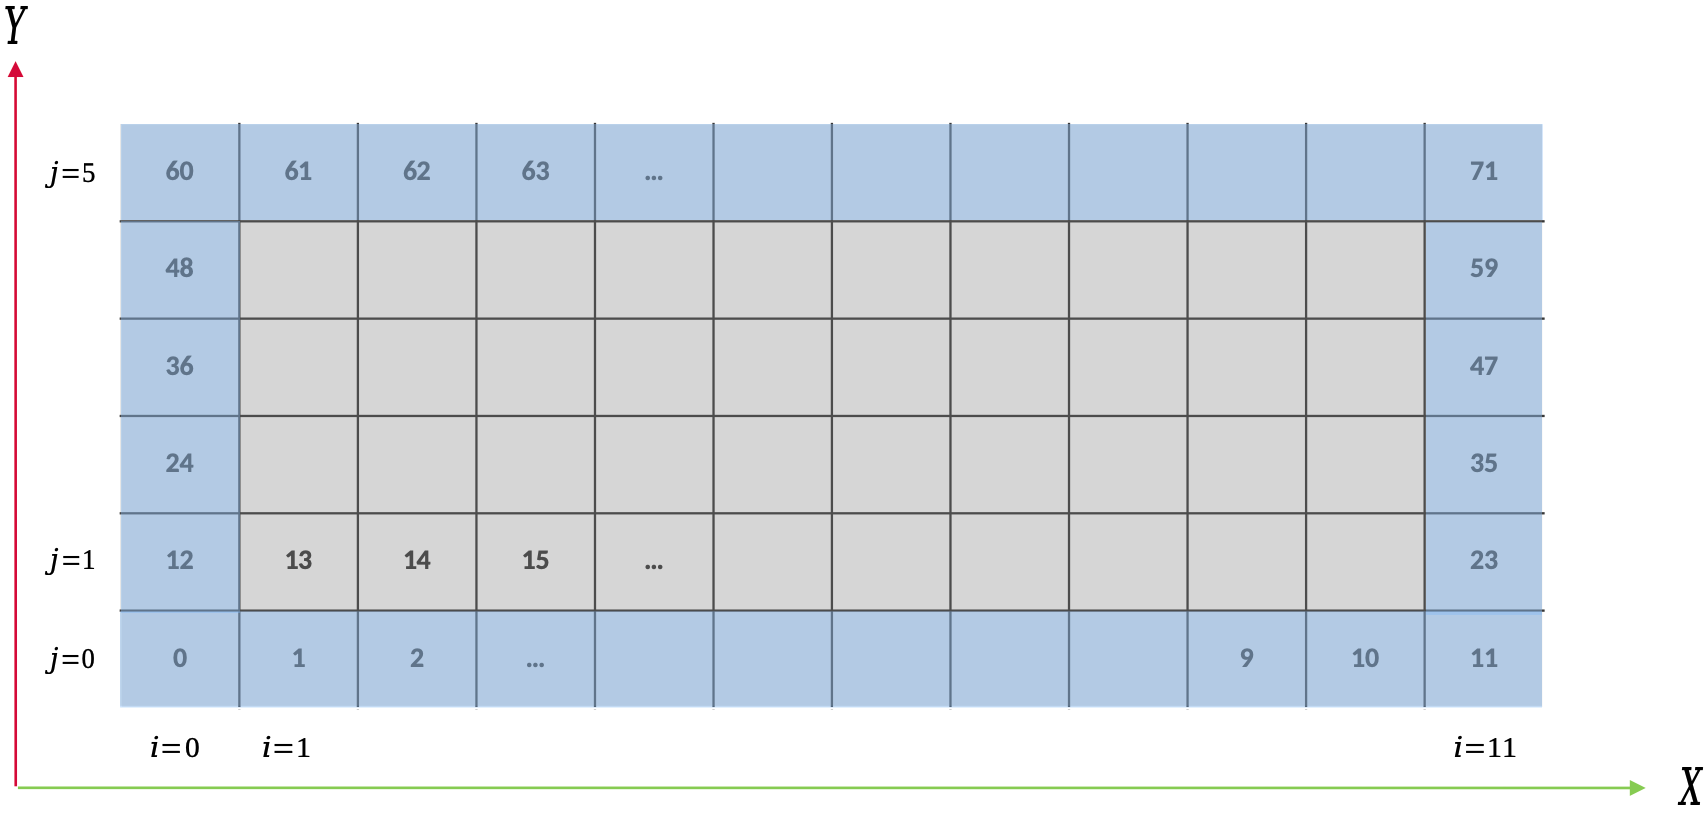
\includegraphics[width=0.75\linewidth]{chapter3_numerical_methods/pictures/grid_ghost_2.png}
    \caption{
        Illustration of the ghost cells layer (blue cells) around the Cartesian grid in HYPERION.
        The numbering of the cells is also shown.
        Note that the three-dimensional Cartesian meshes are handled in the same fashion, with index $i$ in the $X$ direction evolving the fastest, followed by $j$ in the $Y$ direction, then $k$ in the $Z$ direction.
    }
    \label{fig:ghost_cells}
\end{figure}

\subsubsection{Approximate Riemann solvers}\label{sssec:ars}

Once the fields have been reconstructed at each face of each cell (see paragraph~\ref{sssec:interpolations} above), the left/right discontinuous problem (see equation~\eqref{eq:num_approx_flux}) is solved approximately using a Riemann solver.
The most used approximate solvers can be grouped in three large families: Flux Difference Splitting (FDS), Flux Vector Splitting (FVS) and Flux Type Splitting (FTS) \cite{toro2013riemann,qu2021review}.
In HYPERION we focus on two types of solvers in particular, FDS solvers that work as a finite volume method to solve the Riemann problem and FVS Riemann solvers that combine the qualities of the other two families by separating kinematic and acoustic scales.

Several approximate Riemann solvers have therefore been implemented in HYPERION to serve different purpose.
In the present study, similarly to the need for a reconstruction able to handle large and small scales simultaneously, the Riemann solver we were seeking had to have the ability to behave well in both high and low-Mach regimes (see \emph{e.g.} \cite{maier2021su2}) and to not trigger the well-known carbuncle instability\cite{kitamura2012carbuncle}.
% especially in the cases where "dead water" recirculation regions could appear in the flow because of the obstacles.
A series of tests and a bibliographic study lead us to opt in for a FVS solver constructed by Liou \emph{et al.}, the AUSM$^+$-up \cite{liou1996sequel,liou2006sequel} because of its robustness and its increased level of accuracy at all speeds.
Presenting the details of the mathematical implementations is out of the scope of this paper but the interested reader is referred to the aforementioned papers.

\subsection{Sharp immersed boundary conditions}\label{ssec:ibc}

\begin{figure}[ht!]
    \centering
    \begin{tabular}{ccc}
        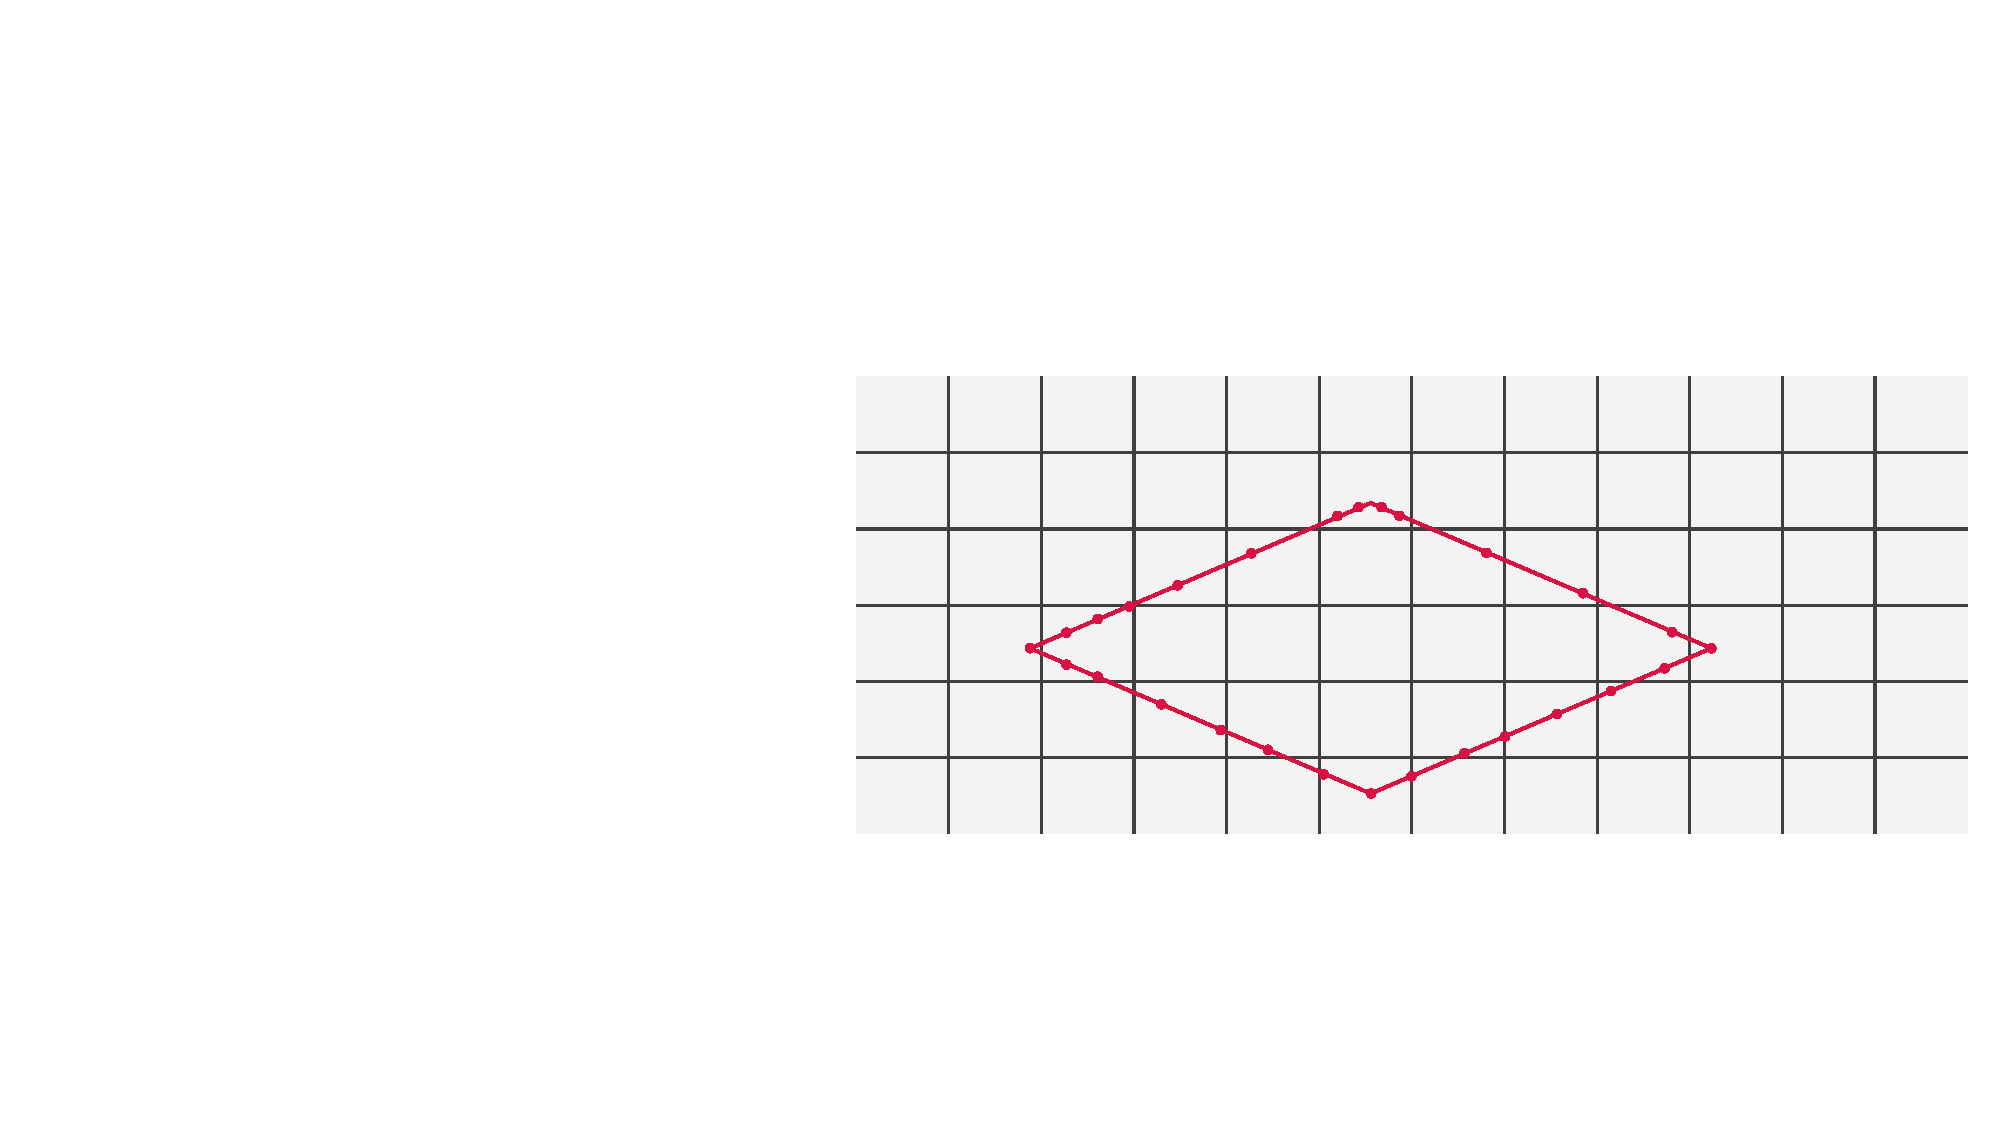
\includegraphics[width=0.3\linewidth]{chapter3_numerical_methods/pictures/ibm1.pdf} &
        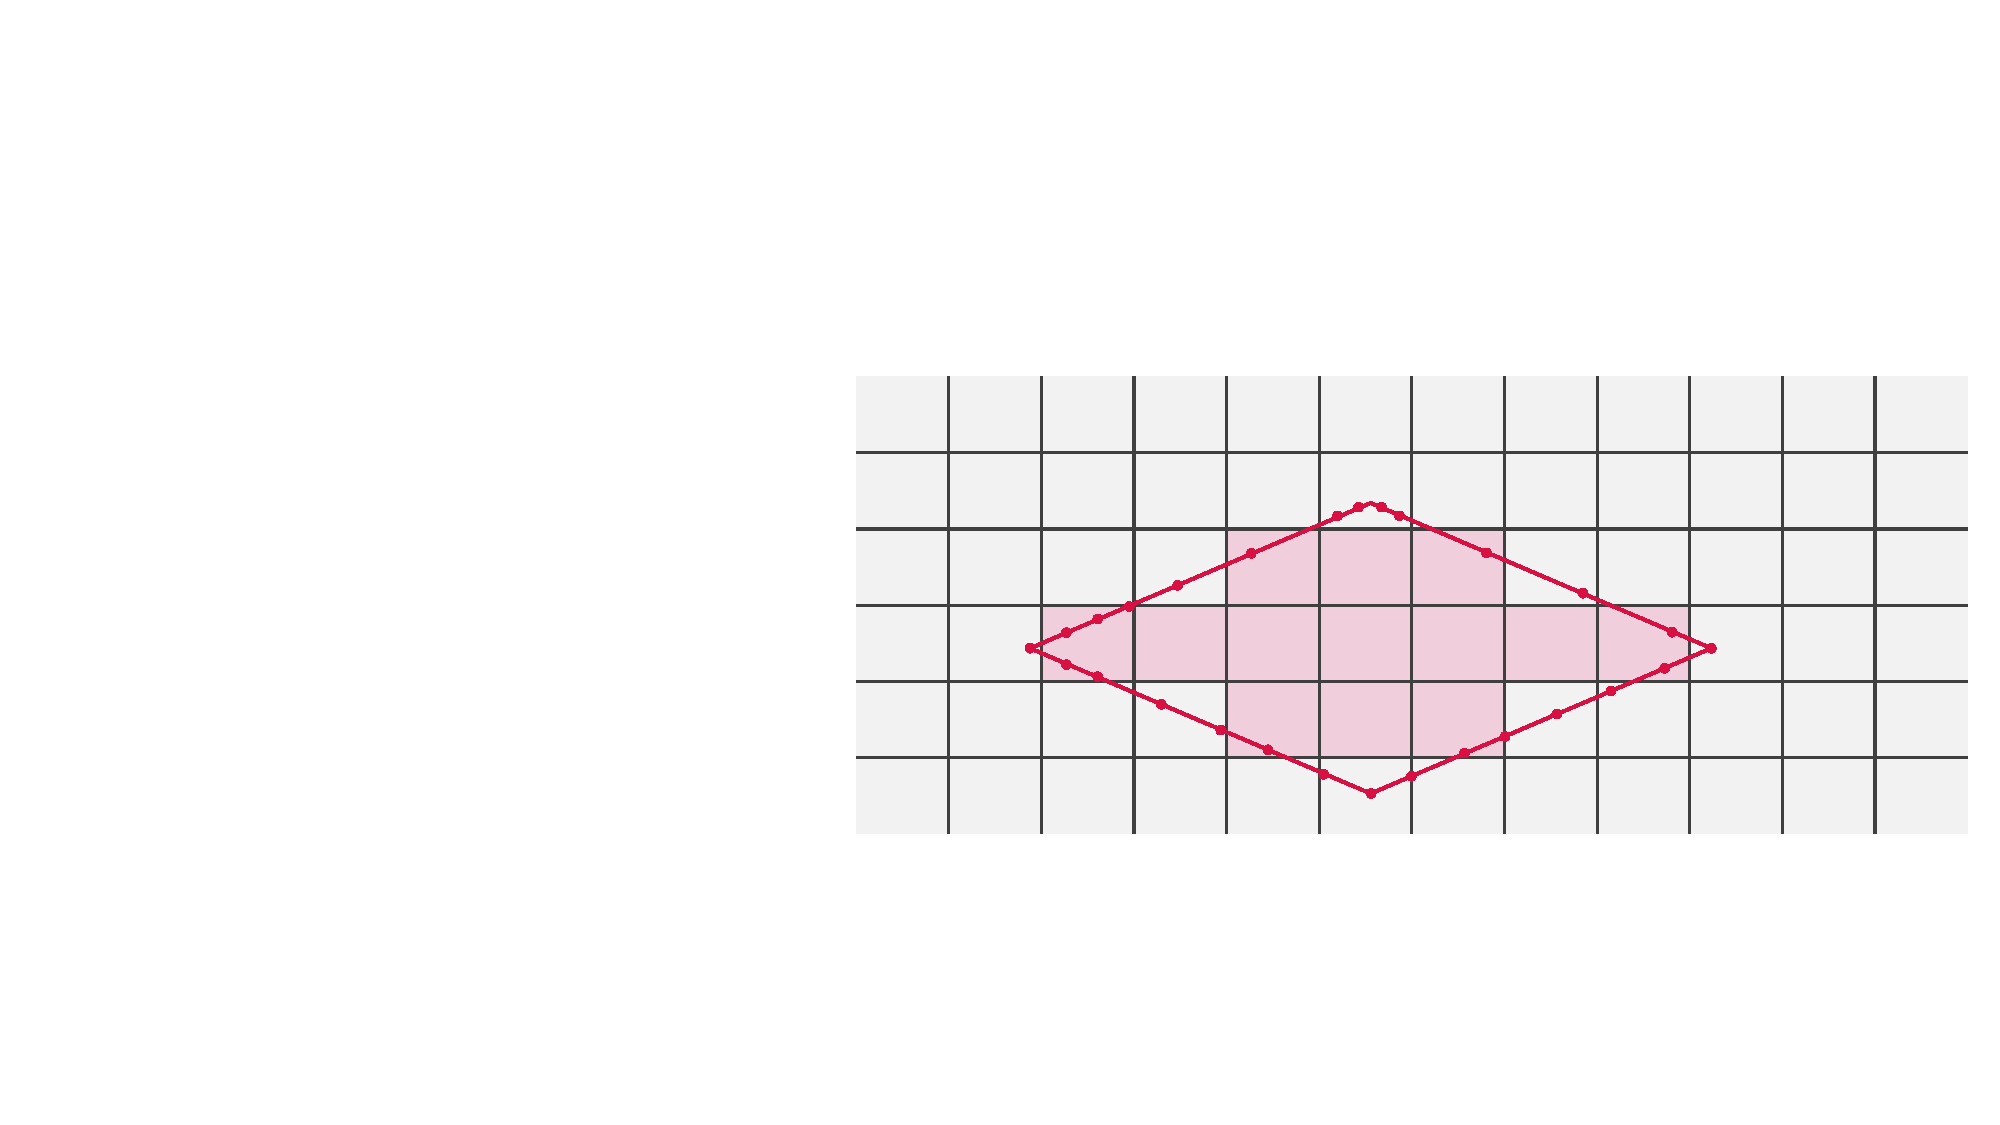
\includegraphics[width=0.3\linewidth]{chapter3_numerical_methods/pictures/ibm2.pdf} &
        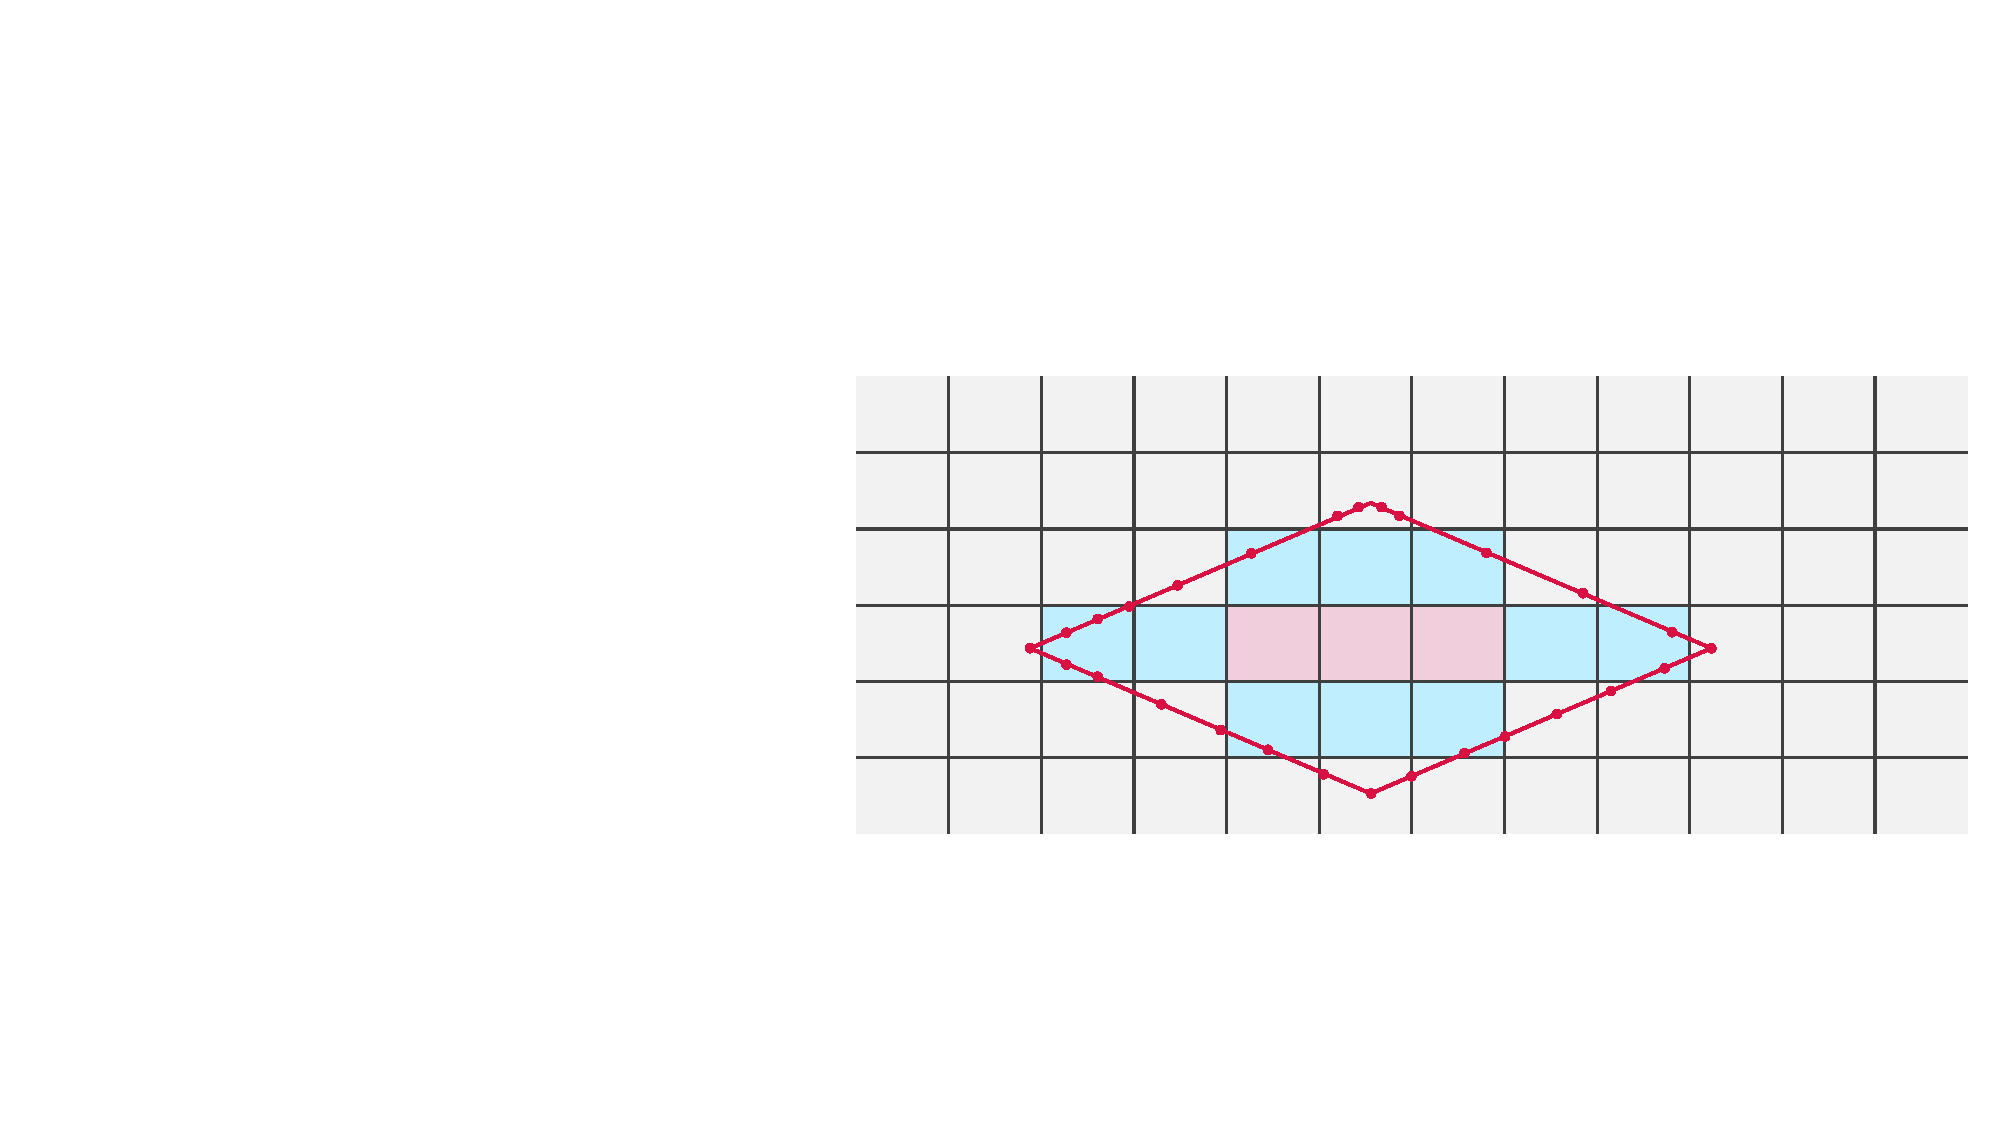
\includegraphics[width=0.3\linewidth]{chapter3_numerical_methods/pictures/ibm3.pdf} \\[0.4em]
        (a) & (b) & (c) \\
        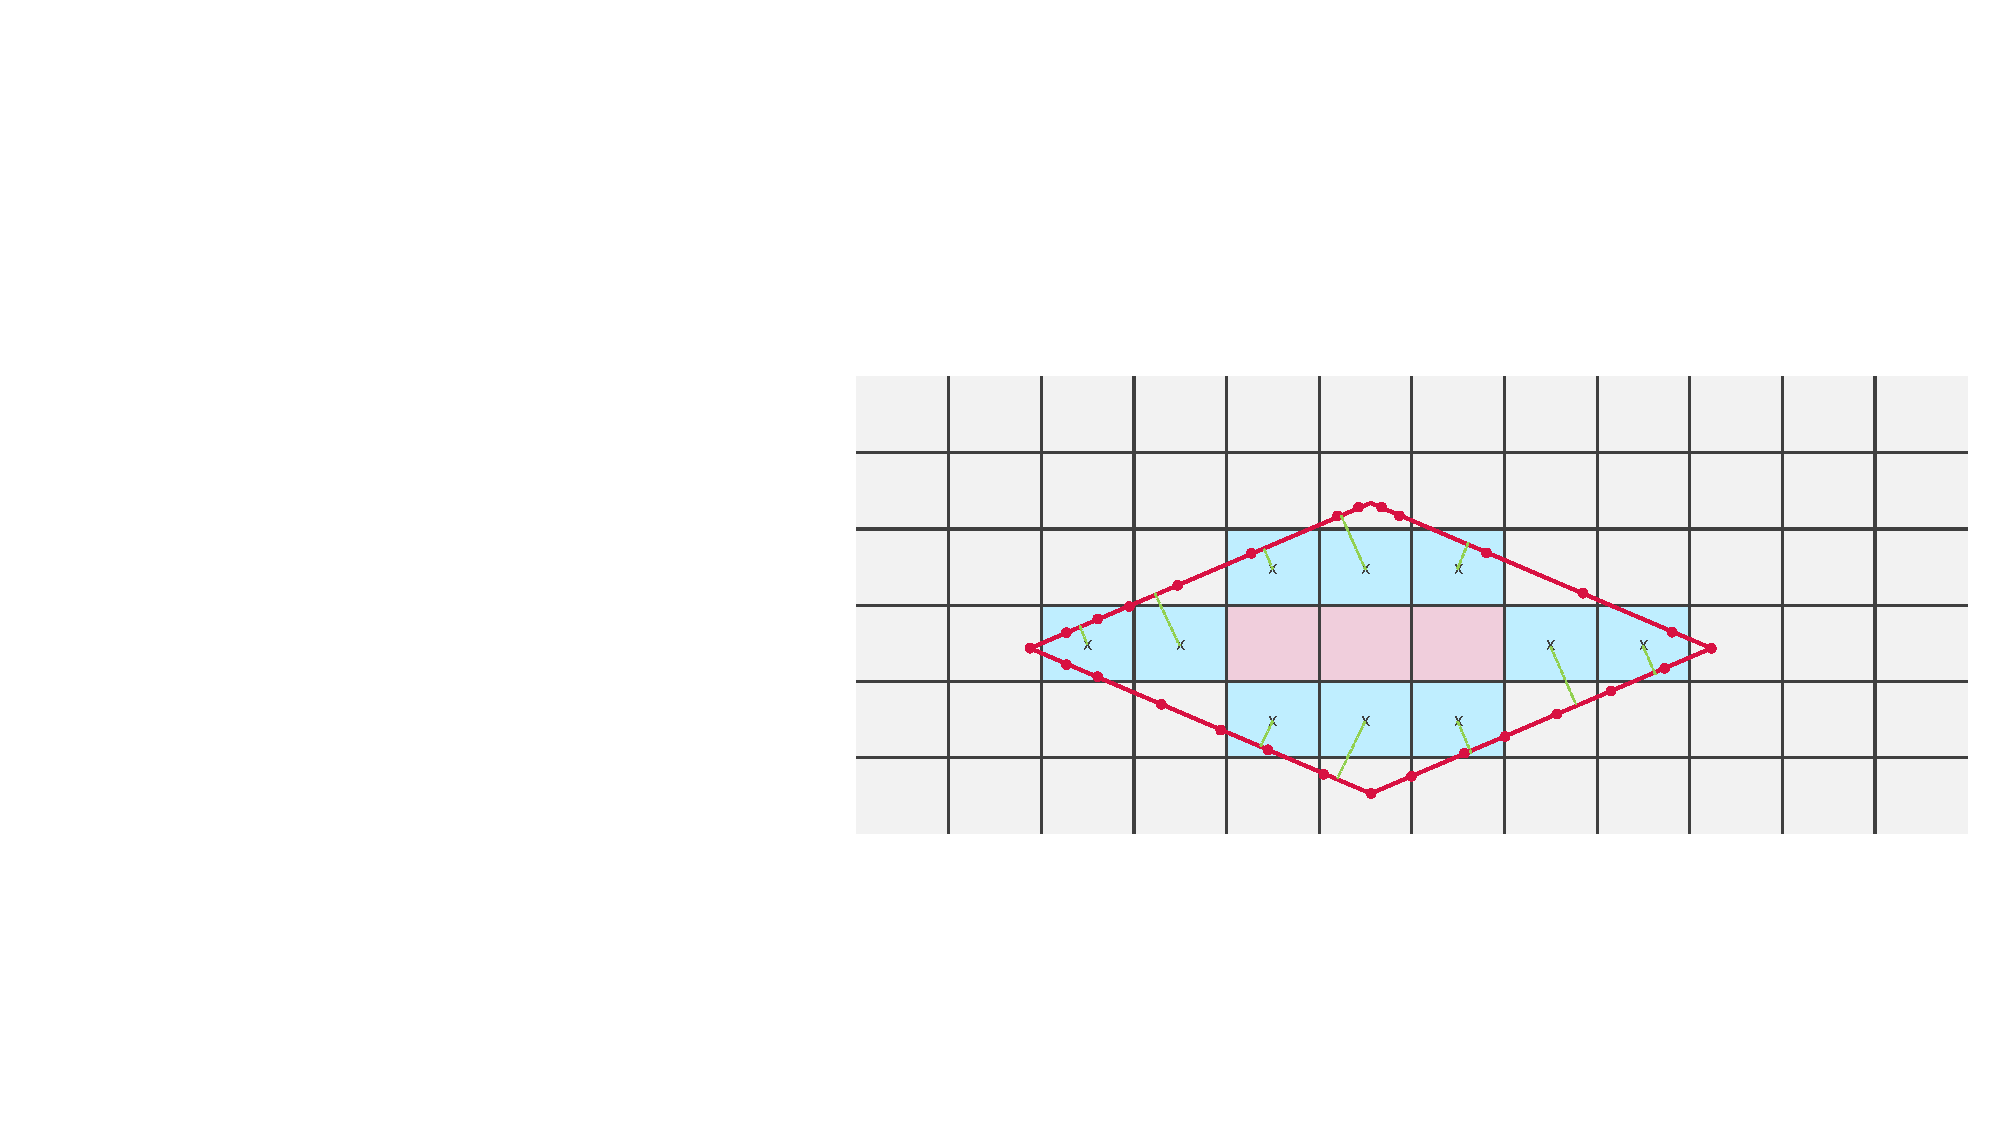
\includegraphics[width=0.3\linewidth]{chapter3_numerical_methods/pictures/ibm4.pdf} &
        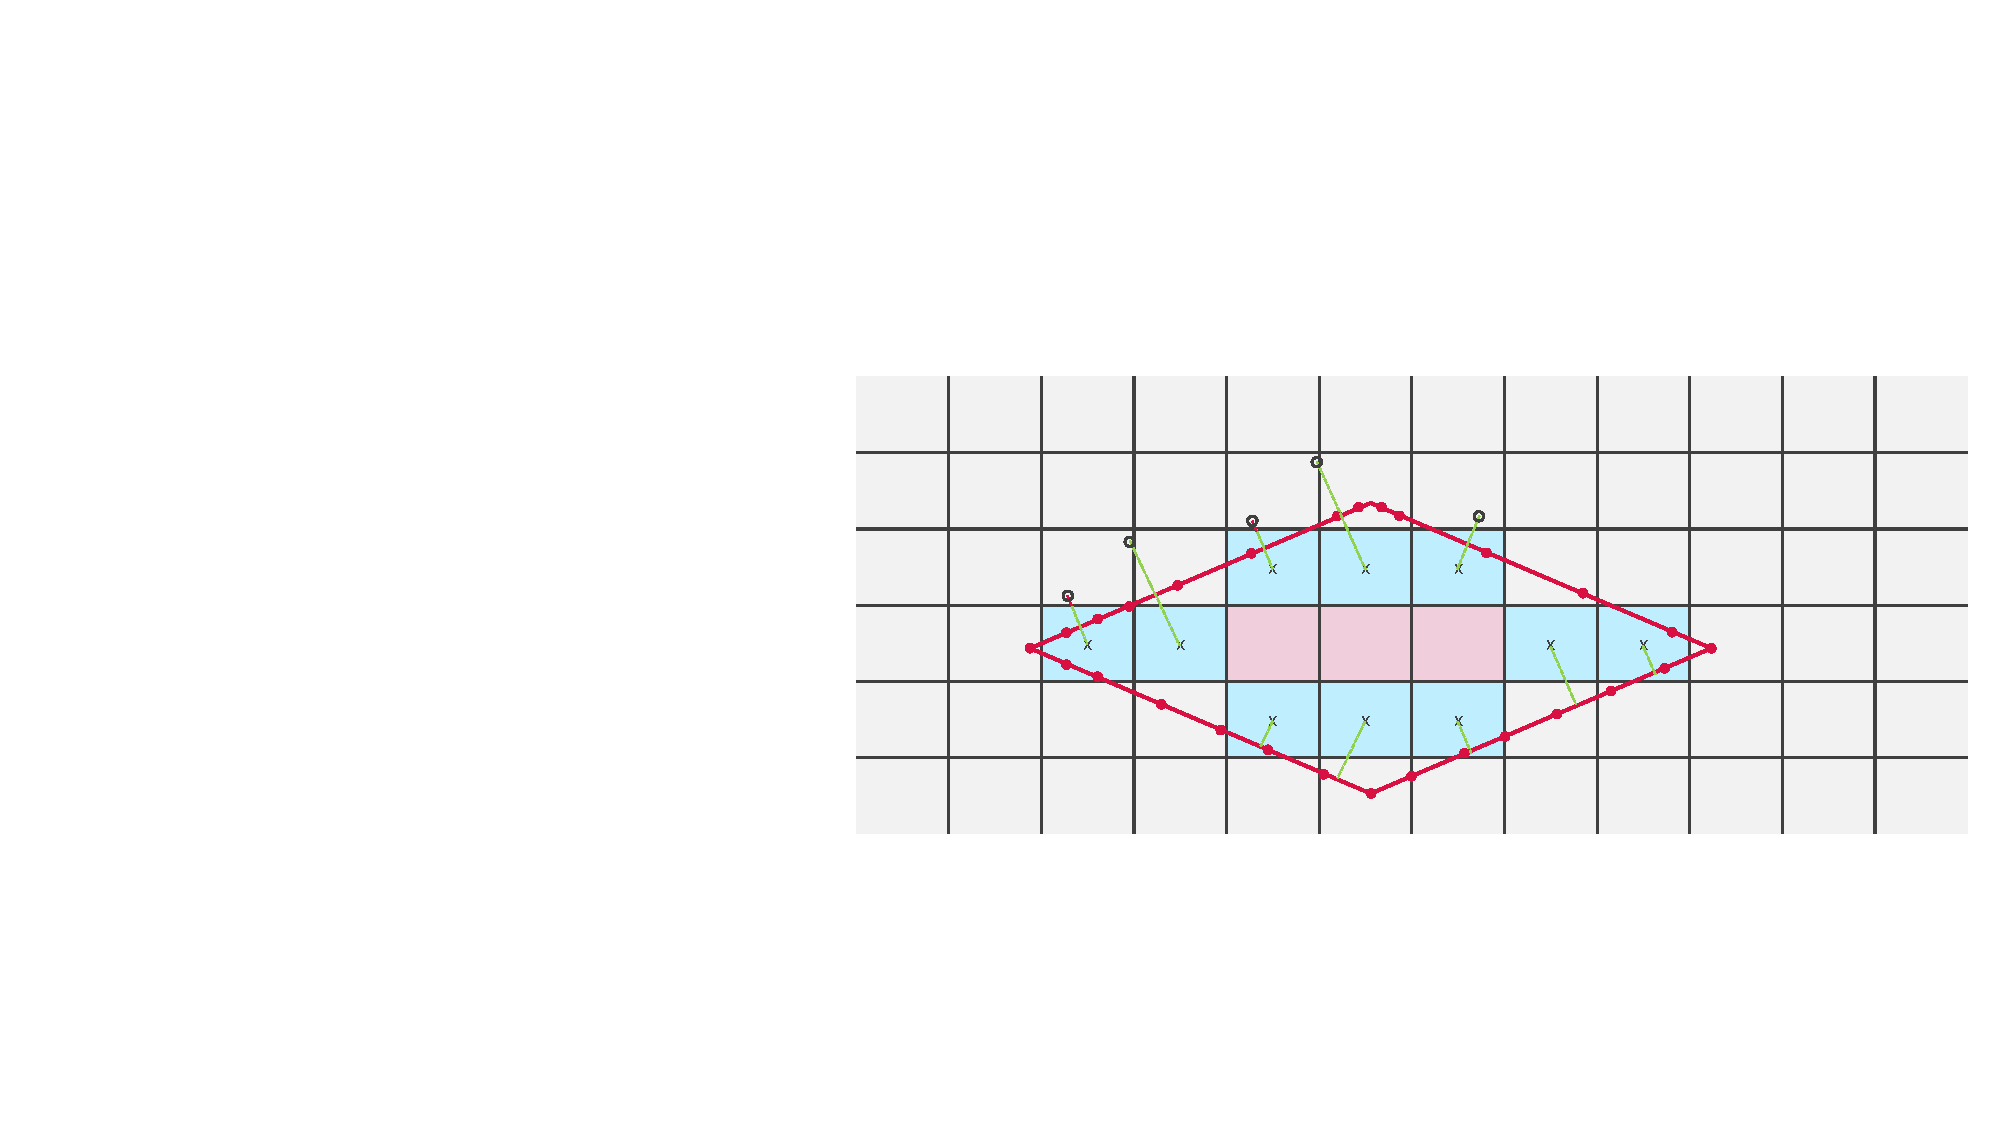
\includegraphics[width=0.3\linewidth]{chapter3_numerical_methods/pictures/ibm5.pdf} &
        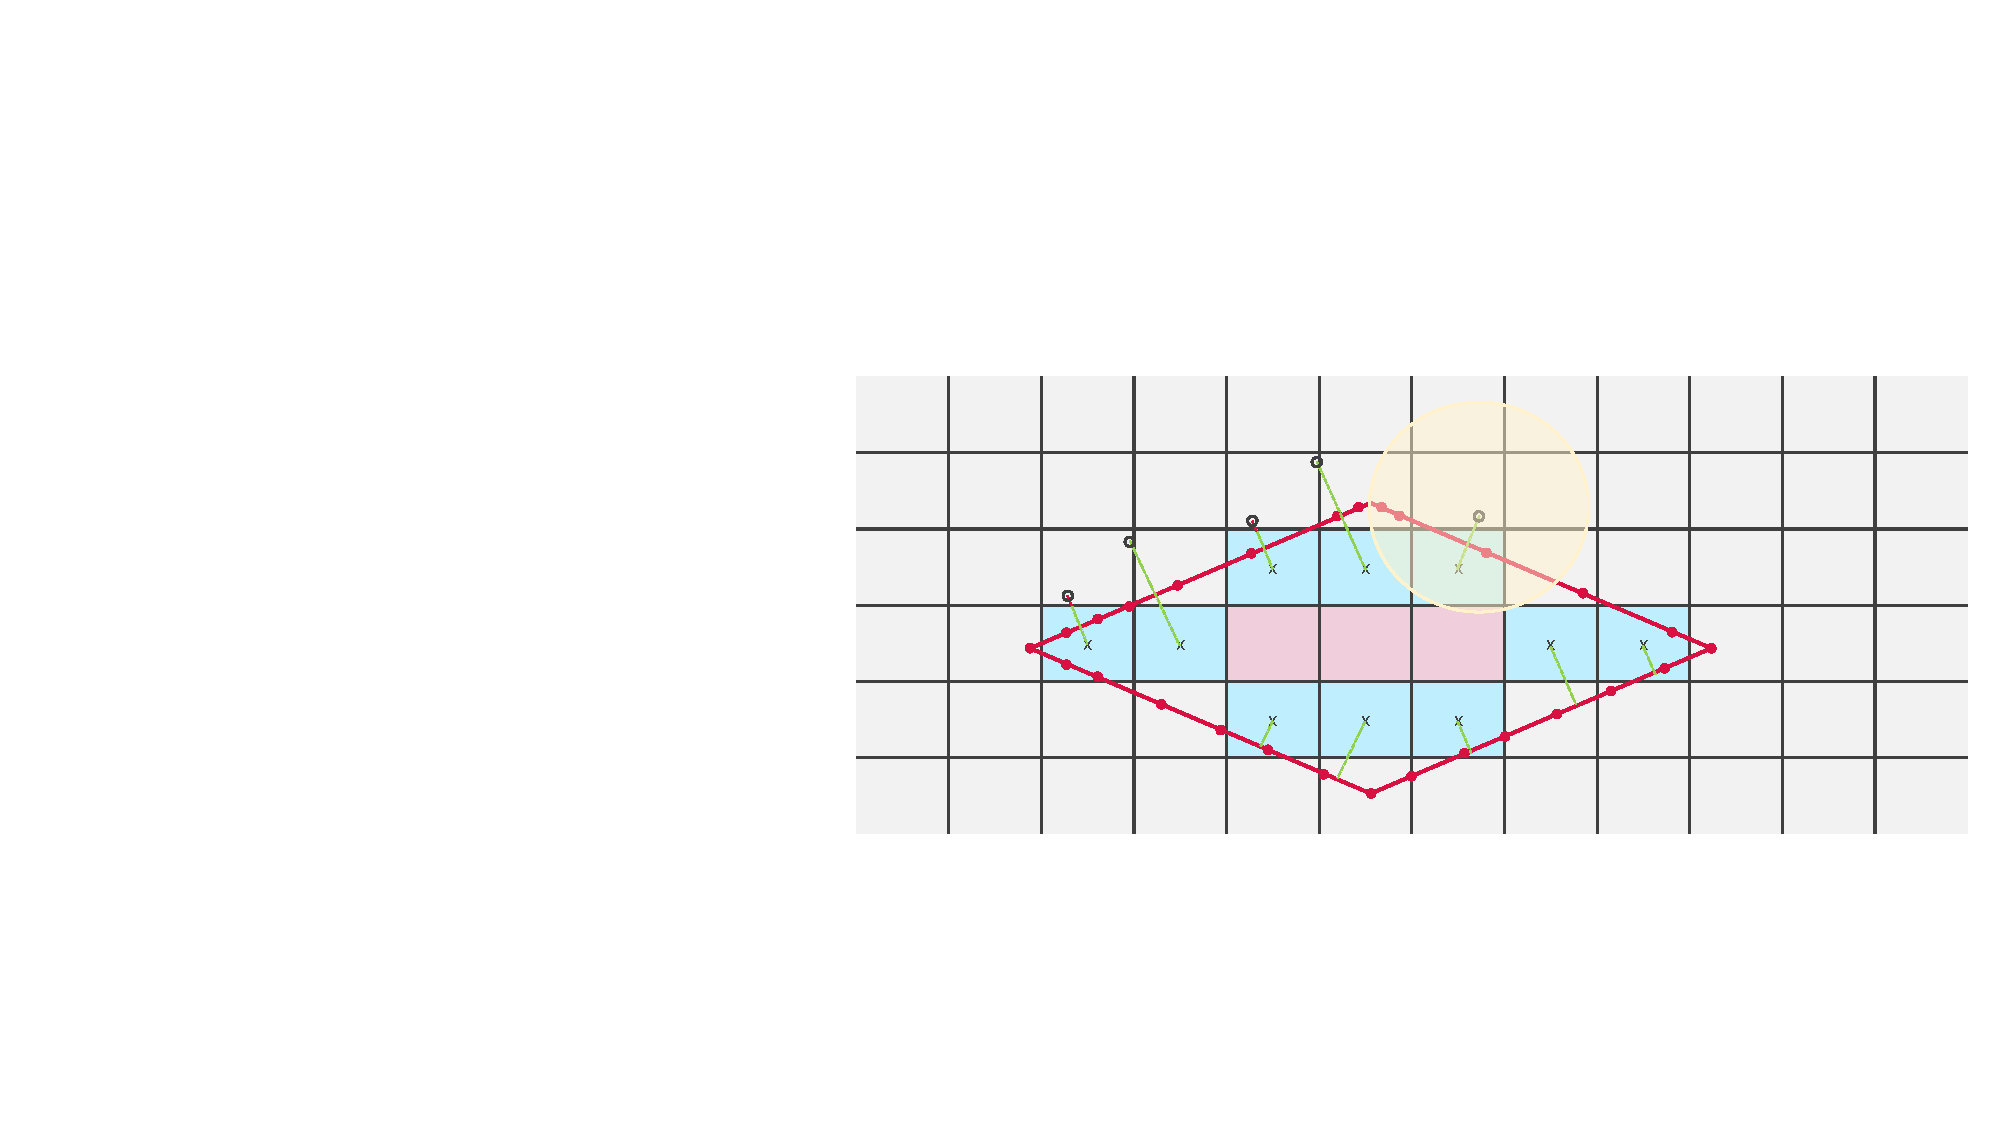
\includegraphics[width=0.3\linewidth]{chapter3_numerical_methods/pictures/ibm6.pdf} \\
        (d) & (e) & (f) \\
        & 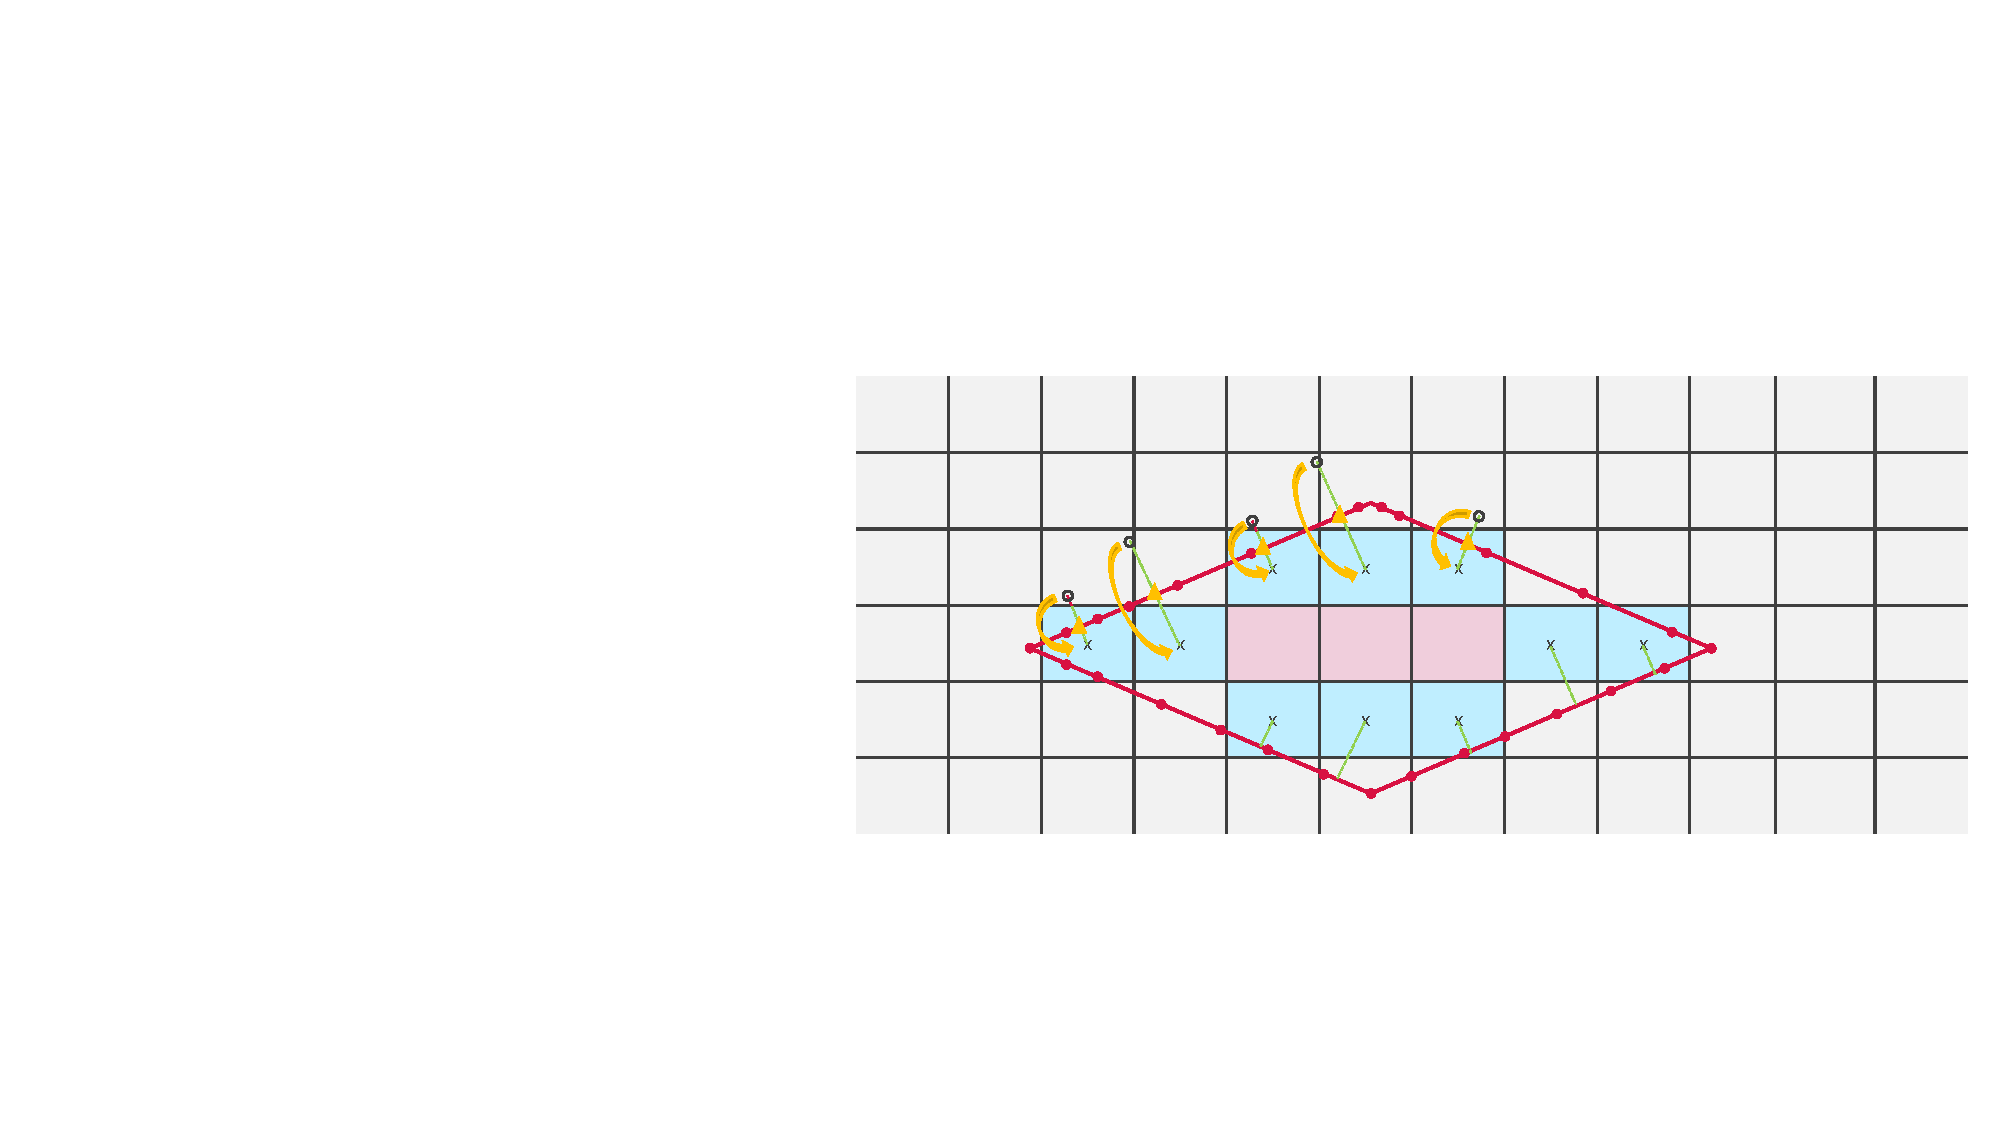
\includegraphics[width=0.3\linewidth]{chapter3_numerical_methods/pictures/ibm7.pdf} & \\
        & (g) &
    \end{tabular}
    \caption{Immersed boundary method workflow - diagrams are shown in two dimensions but the extension to three dimensions in straightforward.
    (a) Introduction of a tesselated object in the Cartesian mesh.
    (b) Detection of the immersed cells (red), $\emph{i.e.}$ solid cells, at initialization.
    (c) Detection of the immersed boundary cells (blue), $\emph{i.e.}$ solid cells with at least one fluid neighbor within the extent of the stencil, at initialization.
    (d) Detection of the nearest facet to each immersed boundary cell, at initialization
    (e) Creation of the image points in the direction normal to the nearest facet for each immersed boundary cell, at initialization.
    (f) Illustration of the neighborhood (yellow) where fluid cells are queried for information to interpolate the values of the fields at the image points, at each iteration of the fluid solver.
    (g) Illustration of the linear extrapolation from the image points to the immersed boundary cells to fill the values allowing for the enforcement of the boundary condition at the wall of the immersed object, at each iteration of the fluid solver.}
    \label{fig:ibm_workflow}
\end{figure}

To handle the presence of obstacles in the compressible flows, HYPERION uses a sharp immersed boundary method (IBM) \cite{mittal2005immersed}.
As mentioned in many papers, \emph{e.g.} \cite{khalili2019,qu2018}, the sharp interface method proves to be well suited for compressible flows because the boundary conditions at the immersed boundary are taken into account directly rather than being computed indirectly \emph{via} a forcing term or smoothed with a distribution function.
Originally, to handle boundary conditions at the edges of the domain, HYPERION uses ghost cells so there is no need to degenerate the reconstruction stencils at the edges.
To make use of the original data structures and logic of implementation as much as possible, we implemented a ghost-cell based immersed boundary method as well.
In the present study, we assume that the immersed objects cannot move.

We will briefly introduce in this section the workflow for the initialization of the immersed boundary method as it will serve as reference for future sections~\ref{sec:rasterization} and~\ref{sec:migratable_tasks}.
Overall the workflow is fairly classical \cite{mittal2005immersed,chi2017improved,khalili2019,qu2018,yousefzadeh2019,zhang2019} and relies on six main steps:

\begin{itemize}
    \item detection of the immersed cells, \emph{i.e.} all the cells of the Cartesian mesh that find themselves \emph{inside} the immersed object - figure~\ref{fig:ibm_workflow}(b),
    \item detection of the immersed boundary cells, that is immersed cells with at least one fluid neighbor within the extent of the reconstruction stencil, and wherein we shall impose the right values to enforce the boundary condition at the wall of the immersed object - figure~\ref{fig:ibm_workflow}(c),
    \item detection of the nearest facet to each immersed boundary cell in the sense of normal projection distance - figure~\ref{fig:ibm_workflow}(d),
    \item computation of the images of each immersed boundary cell center with respect to their nearest facet - figure~\ref{fig:ibm_workflow}(e),
    \item interpolation of the fluid variables at the image points - figure~\ref{fig:ibm_workflow}(f),
    \item linear extrapolation from the image points to the immersed boundary cells to enforce the boundary condition at the wall of the immersed object - figure~\ref{fig:ibm_workflow}(g).
\end{itemize}

In HYPERION, since we assume that all immersed objects are immovable, the four first steps can be done once during the initialization of the computation, whereas the last two steps, depending on the instantaneous state of the fluid, are repeated at each fluid iteration.

Section~\ref{sec:rasterization} will present the novel algorithm used in HYPERION to make the detection of the immersed cells (step 1) particularly inexpensive, even for three-dimensional objects and Cartesian meshes.
Step 2 and 4 are quite straightforward and rely on simple geometrical notions ; to make step 3 efficient however for large Cartesian meshes and finely discretized immersed objects, HYPERION builds a spatial-median Bounding Volume Hierarchy (BVH) of the immersed objects to accelerate the ray-tracing-like queries for nearest facets\footnote{"Find Closest Point on (Tesselated) Surface" library developed by \emph{ingowald} as a spin-off of the OSPRay project - see \url{github.com/ingowald/closestSurfacePointQueries}}.
Step 5 relies on the ENO-like least-square interpolation algorithm developed by one of the authors \cite{BRIDELBERTOMEU2021}, and section~\ref{sec:migratable_tasks} shall detail the strategy implemented in HYPERION to handle the large interpolation neighborhood in a massive parallelism context.
Finally, step 6 is straightforward as well and the interested reader can find all the mathematical details in Bridel-Bertomeu \cite{BRIDELBERTOMEU2021}.

\section{A FAST RASTERIZATION ALGORITHM TO DETECT IMMERSED CELLS}\label{sec:rasterization}
%
% [TBB] Ici on pointe sur (quasiment) la première partie du workflow IBC évoquée précédemment & on décrit l'algo de rasterization
% en 3D basé sur des maillages tétrahédriques des objets immergés et l'équivalence entre ce que nous on appelle un maillage Cartésien
% homogène et ce que la communauté du jeu vidéo appelle un maillage de voxel.
% Il va falloir ressusciter d'une façon ou d'une autre l'ancien algo 3D brute-force pour pouvoir fournir des comparaisons en terme de
% temps de traitement.
%

To identify the solid cells, \emph{i.e.} the cells of the Cartesian mesh that are found \emph{inside} the immersed object, the most common algorithm is a somewhat brute-force ray-casting algorithm (see \emph{e.g} \cite{haines1994point,mittal2005immersed}) that can be described as follows.

\begin{figure}[ht!]
    \centering
    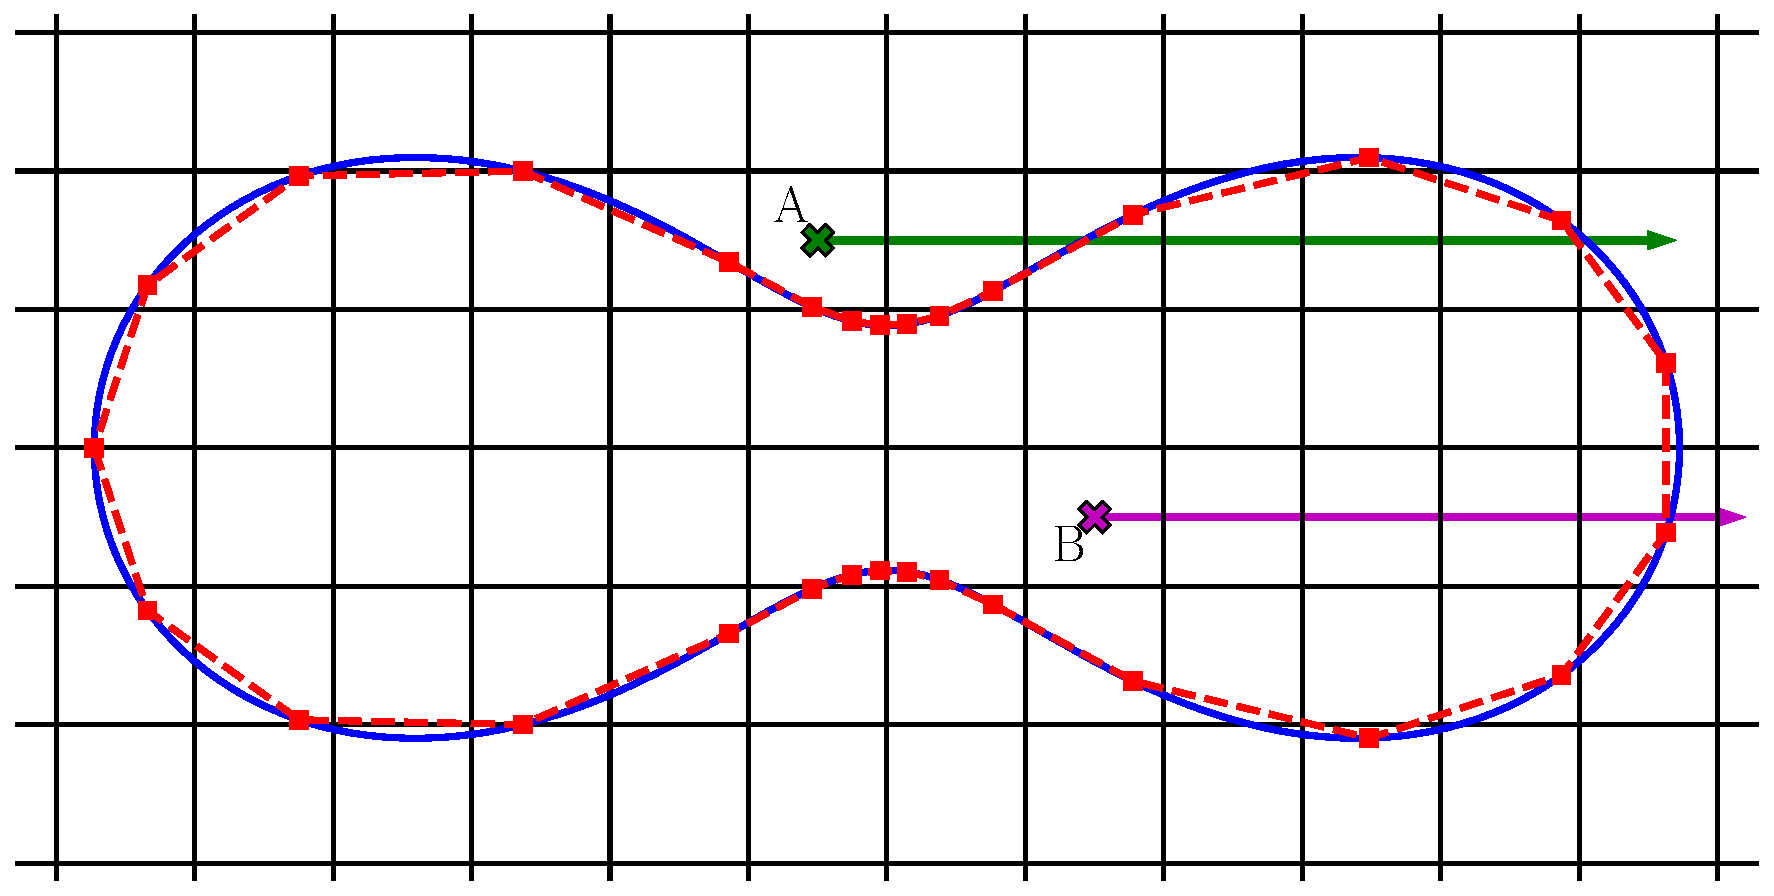
\includegraphics[width=0.7\linewidth]{chapter3_numerical_methods/pictures/cassini_ellipsis.pdf}
    \caption{Illustration of the tesselation of a two-dimensional curve and of the simple ray-casting algorithm for the identification of immersed cells.}
    \label{fig:ray_casting_simple}
\end{figure}

From all cells in the Cartesian mesh a random ray is cast (see for example cells $A$ and $B$ in figure~\ref{fig:ray_casting_simple}, but the ray could go any direction) and the intersections between this ray and the facets of the body are counted.
If the number of intersections is odd, then the cell wherefrom the ray is cast is inside the immersed body (for example cell $B$) whereas if the number of intersections is even, the originating cell is outside the immersed body (for example cell $A$).
The complexity of this algorithm is $\mathcal{O}\left( N_c N_f\right)$, where $N_c$ is the total number of cells in the Cartesian mesh and $N_f$ is the total number of facets of the tesselated immersed body. \\
For two-dimensional problems, such a complexity hardly becomes an issue.
As an illustration, let us nonetheless consider a three-dimensional worst case with a Cartesian mesh of $900 \times 900 \times 1300$ cells and an object with approximately $5\times 10^5$ facets, then the algorithm runs for more than $48$ hours on a mid-2017 Intel i7 processor with $4$ OpenMP threads.
Naturally if the Cartesian mesh is partitioned, then each partition handles its own set of rays and the time-to-completion drops to the order of magnitude of tens of minutes, but it still is not a reasonable performance - especially if one thinks of the possibility of having a moving object, for which the solid cells might change at each iteration of the fluid solver.

The technical name of the "problem that consists in finding the solid cells" is \emph{point classification}: in our case, we want to classify the cell centers according to whether they are inside or outside some shell.
\emph{Point classification} problems fall within the theory of computational geometry, which pushed the second author to associate himself with David Eberly \cite{schneider2002geometric} from Geometric Tools\footnote{See \url{https://www.geometrictools.com} for more information about the company} to develop a better algorithm than the aforementioned brute-force one - this section is dedicated to the presentation of this new algorithm.

The ray-casting algorithm simply needs the immersed object to be defined by the discretization of its outermost shell - a segment-based tesselation in two dimensions or a triangle-based tesselation in three dimensions.
The new algorithm relies on a tesselation of the outermost shell \emph{and} on the existence of a tetrahedralization (triangulation) of the inside of the object in three (two) dimensions - this shift in paradigm is illustrated on figure~\ref{fig:object_discretization}.

\begin{figure}
    \centering
    \begin{tabular}{cc}
        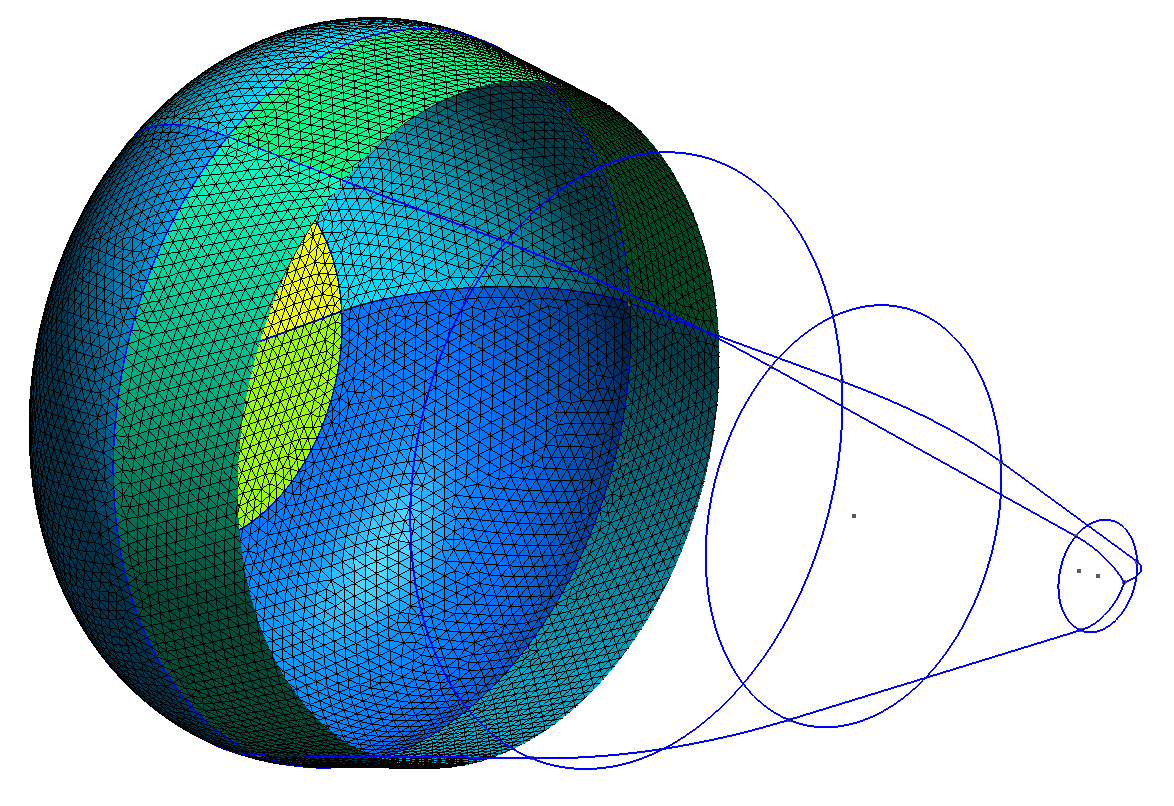
\includegraphics[width=0.45\linewidth]{chapter3_numerical_methods/pictures/funny_onion_shell.png} &
        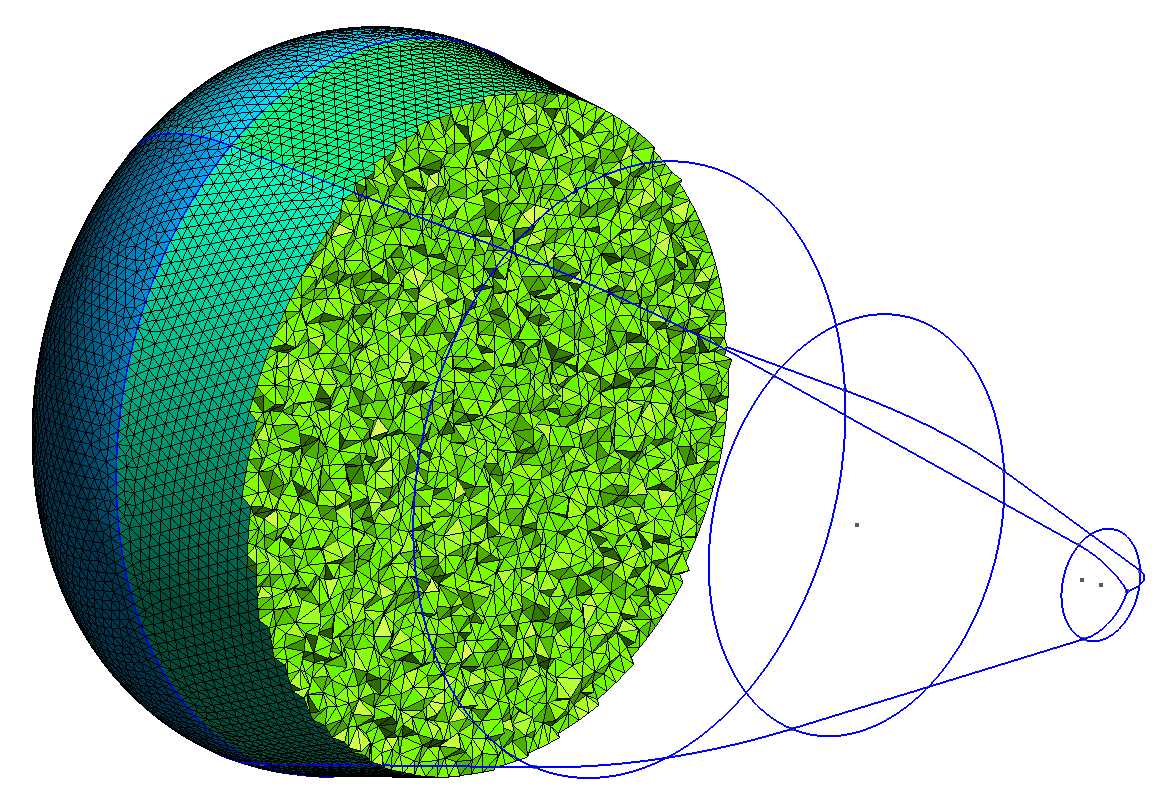
\includegraphics[width=0.45\linewidth]{chapter3_numerical_methods/pictures/funny_onion_threeD.png} \\
        (a) & (b)
    \end{tabular}
    \caption{Discretization of the immersed objects necessary (a) for the simple ray-casting algorithm and (b) for the new \emph{point classification} algorithm.
    The three-dimensional tetrahedralization required by the new algorithm has to be generated beforehand and is not handled by HYPERION.}
    \label{fig:object_discretization}
\end{figure}

Once a proper tetrahedralization (triangulation) has been obtained, the algorithm has the following steps - note that a description is provided in the three-dimensional case but the algorithm applies similarly in two dimensions.

\begin{itemize}
    \item[$\bullet$] Step 1 - for each tetrahedron, create its smallest axis-aligned bounding box (AABBs).

\begin{verbatim}
        function compute tetrahedra AABB
            for each tetrahedron t
                v1, v2, v3, v4 := the four vertices of the t
                t_min := v1
                t_max := t_max
                for each vertex v
                    for each dimension d
                        if coordinate d of v < coordinate d of t_min
                        then
                            coordinate d of t_min := coordinate d of v
                        else if coordinate d of v > coordinate d of t_max
                        then
                            coordinate d of t_max := coordinate d of v
                        end if
                    end for each
                end for each
            end for each
        end function
\end{verbatim}

    \item[$\bullet$] Step 2 - each AABB is clipped/culled against the underlying Cartesian mesh to ensure that when searching within the bounding boxes, the grid points are within range of the Cartesian mesh bounds. Note that the "underlying Cartesian mesh" can very well be a local piece of mesh in the context of MPI partitioning, making this \emph{point classification} inherently adapted to distributed parallelism.

\begin{verbatim}
        function cull tetrahedra AABB
            m_min, m_max := lower, upper vertex of Cartesian box
            for each tetrahedron t
                t_min, t_max := lower, upper vertex of t bounding box
                for each dimension d
                    coordinate d of t_min :=
                        max between
                            | coordinate d of t_min,
                            | coordinate d of m_min
                    coordinate d of t_max :=
                        min between
                            | coordinate d of t_max,
                            | coordinate d of m_max
                    if coordinate d of t_min > coordinate d of t_max
                    then
                        declare t invalid
                    end if
                end for each
            end for each
        end function
\end{verbatim}

    \item[$\bullet$] Step 3 - the tetrahedra vertices and bounding boxes are then transformed to the $(i,j,k)$ grid coordinate system.

\begin{verbatim}
        function transform to grid ijk
            m_min, m_max := lower, upper vertex
                of Cartesian box
            n.0, n.1, n.2 := number of cells
                of Cartesian box in each dimension
            for each dimension d
                factor.d := (n.d - 1) / (
                    coordinate d of m_max -
                    coordinate d of m_min
                )
            end for each
            for each tetrahedron t
                t_min, t_max := lower, upper vertex
                    of t bounding box
                for each dimension d
                    g_t_min := ceiling of factor.d * (
                        coordinate d of t_min -
                        coordinate d of m_min
                    )
                    g_t_max := floor of factor.d * (
                        coordinate d of t_max -
                        coordinate d of m_min
                    )
                end for each
            end for each
        end function
\end{verbatim}

    \item[$\bullet$] Step 4 - each grid-coordinate bounding box contains a relatively small number of the Cartesian grid cell centers, hence we can iterate over those with a triple loop in $k$, then $j$, then $i$ as per HYPERION grid ordering. For a constant $(j,k)$ in the grid box, a line segment containing cell centers with varying $i$ is obtained. Note that one possible implementation of the function determining whether a point is in a tetrahedron can be found in \cite{schneider2002geometric} and shall not be repeated here.

\begin{verbatim}
    function rasterize
        n.0, n.1, n.2 := number of cells
            of Cartesian box in each dimension
        for each tetrahedron t
            g_t_min, g_t_max := lower, upper vertex
                of t bounding box in ijk coordinates
            for k from g_t_min.2 to g_t_max.2
                for j from g_t_min.1 to g_t_max.1
                    for i0 from g_t_min.0 to g_t_max.0
                        if (i0,j,k) in tetrahedron t
                        then
                            break for i0
                        end if
                    end for
                    if i0 > g_t_max.0
                    then
                        cycle for j
                    end if
                    for i from g_t_max.0 down to i0
                        if (i,j,k) in tetrahedron t
                        then
                            break for i
                        end if
                    end for
                    base := n.0 * (j + n.1 * k)
                    for l from i0 to i
                        n := l + base
                        flag cell center of index n
                            as inside tetrahedron t
                    end for
                end for
            end for
        end for each
    end function
\end{verbatim}

    \item[$\bullet$] Step 5 - the $i$-values are searched for the first and last cell centers that are inside each tetrahedron, if any, which yields a set of flagged $(i,j,k)$ that can be said to be inside the immersed object.
\end{itemize}

As mentioned, the algorithm can be easily adapted to a code working in parallel.
For a multithreaded code, then the tetrahedra can be split among the different threads to share the workload.
There is a chance that two threads might try to flag the same $(i,j,k)$ to the set of solid cells.
In particular this can happen if a cell center is on the shared face of a pair of tetrahedra (or close to that face because of numerical rounding errors).
However, there is no need for a critical section or an atomic write: first, from the perspective of either thread the cell center will be found to be inside the immersed object, and anyway the $(i,j,k)$ grid coordinates are $32$-bit integers that are written atomically by nature. \\
If the number of tetrahedra in the discretization of the object is noted $N_t$, then the complexity of this algorithm is, mostly, $\mathcal{O}(N_t)$.
For the same worst-case problem as before, the time-to-completion falls to $8.5$ seconds on a single OpenMP thread and the timings for $2$, $4$, $8$ and $16$ OpenMP threads are $4.3$ seconds, $2.6$ seconds, $2.1$ seconds and $2.0$ seconds respectively (versus $\gtrsim 48$ hours for the brute-force algorithm for $4$ OpenMP threads).

\section{MIGRATABLE TASKS FOR THE MASSIVE PARALLELIZATION OF THE RECONSTRUCTION ALGORITHM}\label{sec:migratable_tasks}

As mentioned in section~\ref{ssec:ibc}, the interpolation of the fluid values at each image point (step 5) relies on the least-square ENO-like interpolation discussed in details in the paper by Bridel-Bertomeu \cite{BRIDELBERTOMEU2021}.
A short study in the latter paper mentions that for the algorithm to be robust (\emph{i.e} for the least-square matrix to be well enough conditioned), at least 25 neighbors are necessary in two dimensions for a third order interpolation.
The same kind of study conducted in three dimensions shows that at least 85 neighbors are required for a third order interpolation so that the least-square matrix reaches its asymptotic minimum conditioning.

Furthermore, to balance the number of neighbors picked in each direction around the cell of interest, HYPERION implements a spiral walk (see \cite{BRIDELBERTOMEU2021}, figure~4(a)): with that strategy, getting to 25 (85) neighbors in two (three) dimensions means having access to at least three layers of cells around the cell of interest.
However, considering that such cells of interest are by nature in proximity to the immersed objects and because we cannot consider the immersed cells as valid neighbors in the interpolation, acquiring the information from enough valid neighbors can quickly lead to accessing the fifth or sixth layer of cells away from the cell of interest (\emph{e.g.} for fourth or fifth order interpolation matching the order of the TENO reconstruction described in paragraph~\ref{sssec:interpolations}).

In a sequential, or even in a shared-memory parallelism context, accessing cells that are far away from the cell of interest is not a challenge - the algorithm presented in \cite{BRIDELBERTOMEU2021} could be implemented directly without any modifications in a purely sequential or only OpenMP version of HYPERION.
In a distributed parallelism context however, things become rather tricky if one aims at minimizing the computational overhead related to communications between processes and/or the overall memory use of the application, as is the goal for HYPERION.

\begin{figure}[ht!]
    \centering
    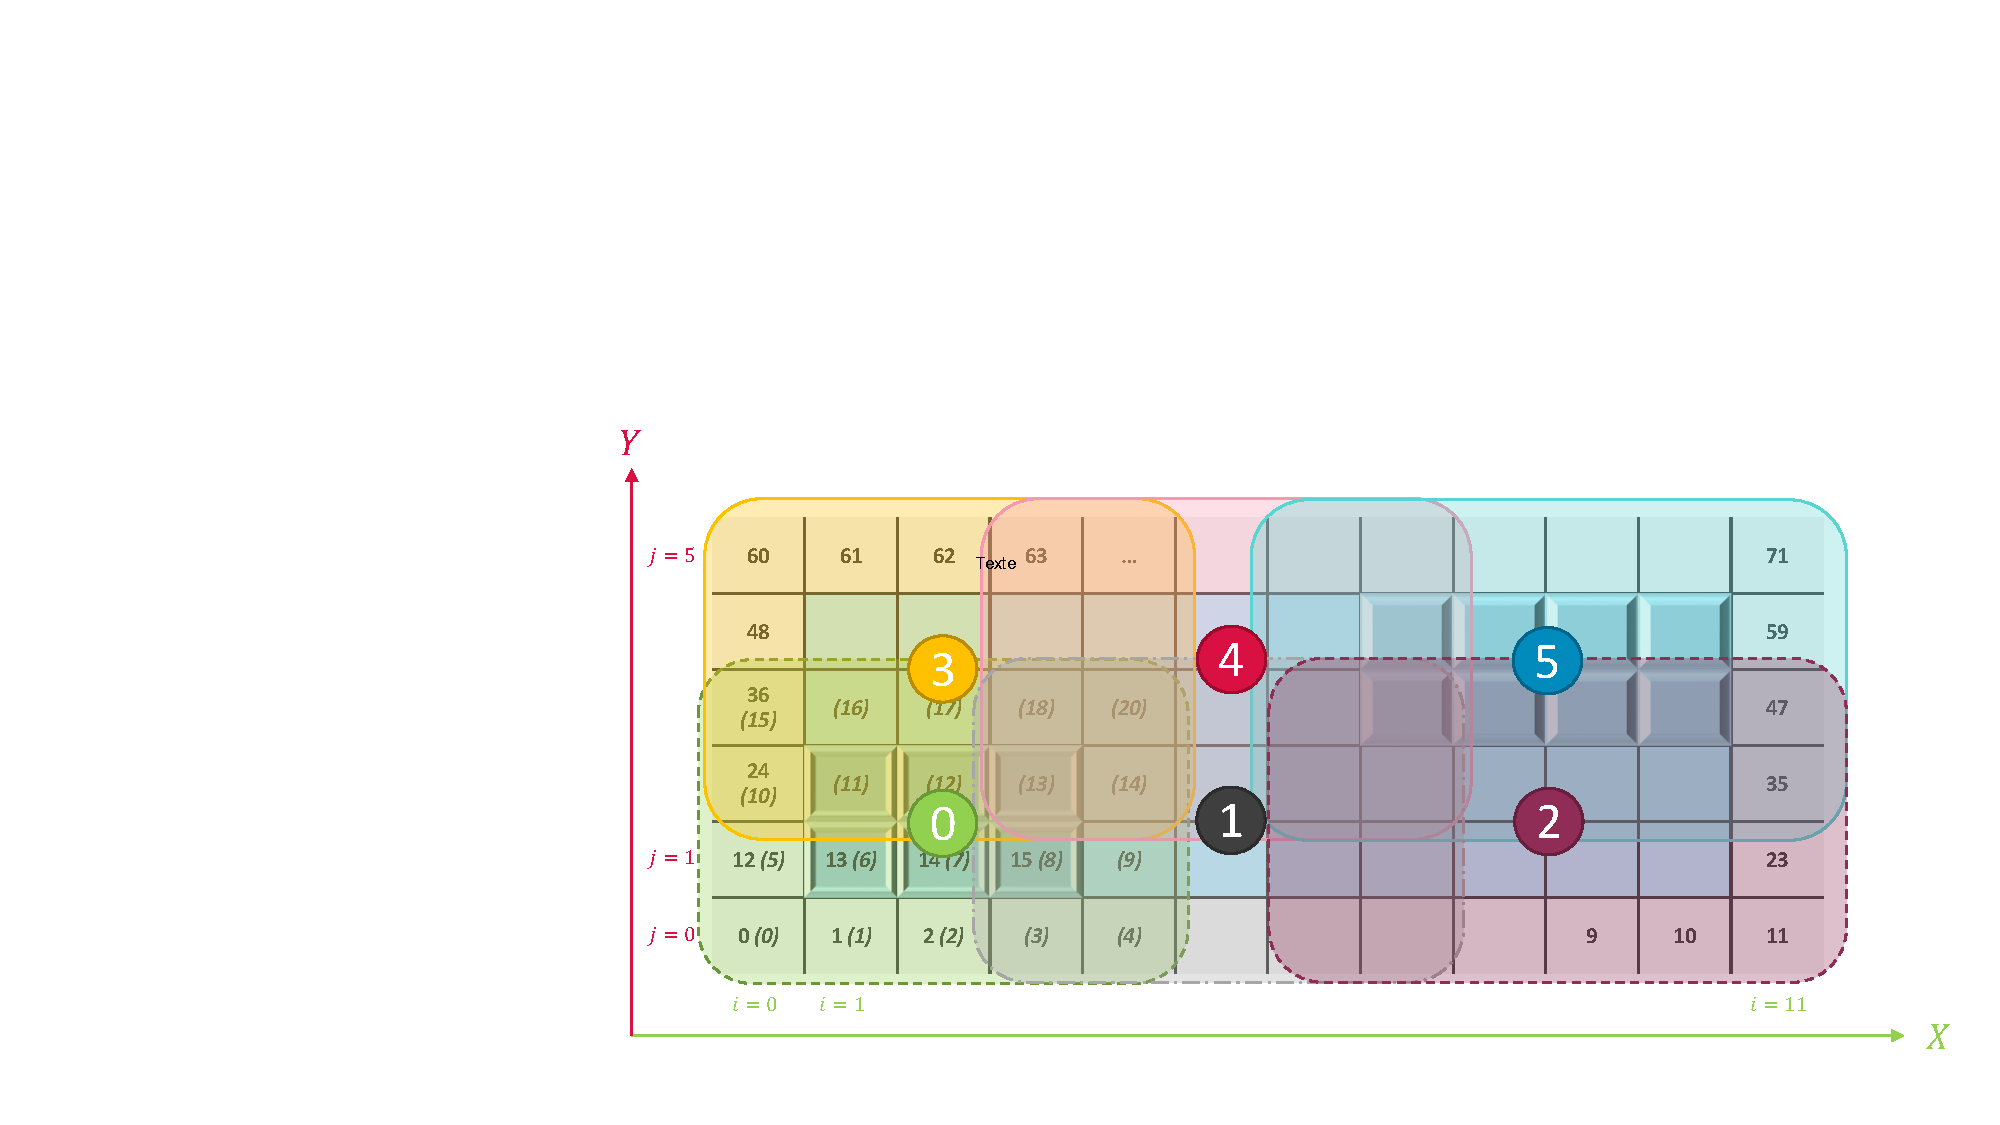
\includegraphics[width=0.75\linewidth]{chapter3_numerical_methods/pictures/mpi_halo.pdf}
    \caption{Illustration of the Cartesian partitioning of the Cartesian mesh in HYPERION.
    The overlapping halos (of size 1 in this case) ensuring communications between neighboring processes are also represented.
    Note that the numbering of the MPI processes is done the same way as the numbering of the fluid cells.}
    \label{fig:mpi_halos}
\end{figure}

If only in terms of memory use, note that out of consistency, in HYPERION the size of the MPI halo equals the number of ghost cells used at the edges of the domain - see figure~\ref{fig:mpi_halos}.
Therefore, if we consider a rather common mesh size of $512^3$ cells, and if we attempt to gain access to cells six layers away with a halo of size $6$, the actual mesh handled by HYPERION has size $(512 + 2 \times 6)^3$, which, if we only account for the five conservative variables, means an overhead of about $3$ Gi in memory.
HYPERION efficiency is around $1$ to $1.5$ $\mu$s$_{\text{CPU}}$/it/cell, hence using a size $6$ halo tends to introduce an overhead of about $10$ s$_{\text{CPU}}$ at each iteration.

With these considerations in mind, along with the fact that having \emph{e.g.} size $6$ halos is highly detrimental to the performance of the MPI communications (although it has not been quantitatively evaluated in the present study), we worked on an algorithm that would not rely on the MPI halos at all in order to perform well in conjunction with any kind of reconstruction stencil.
% that would perform well even with the tighter size $3$ halos required by the TENO reconstruction scheme.
Inspired by the spiral "walk" used in a sequential context to gather information from enough valid neighbors for the least-square interpolation, we turned ourselves towards a migratable task paradigm. \\
In this paradigm, the first ingredient is a \emph{task}.
In our context, let us remember that for each image point we want to gather information from enough "valid" neighbors to have a well-conditioned least-square matrix (see figures~\ref{fig:ibm_workflow}(f) and~\ref{fig:migratable_task}(a)).

\begin{figure}[ht!]
    \centering
    \begin{tabular}{cc}
        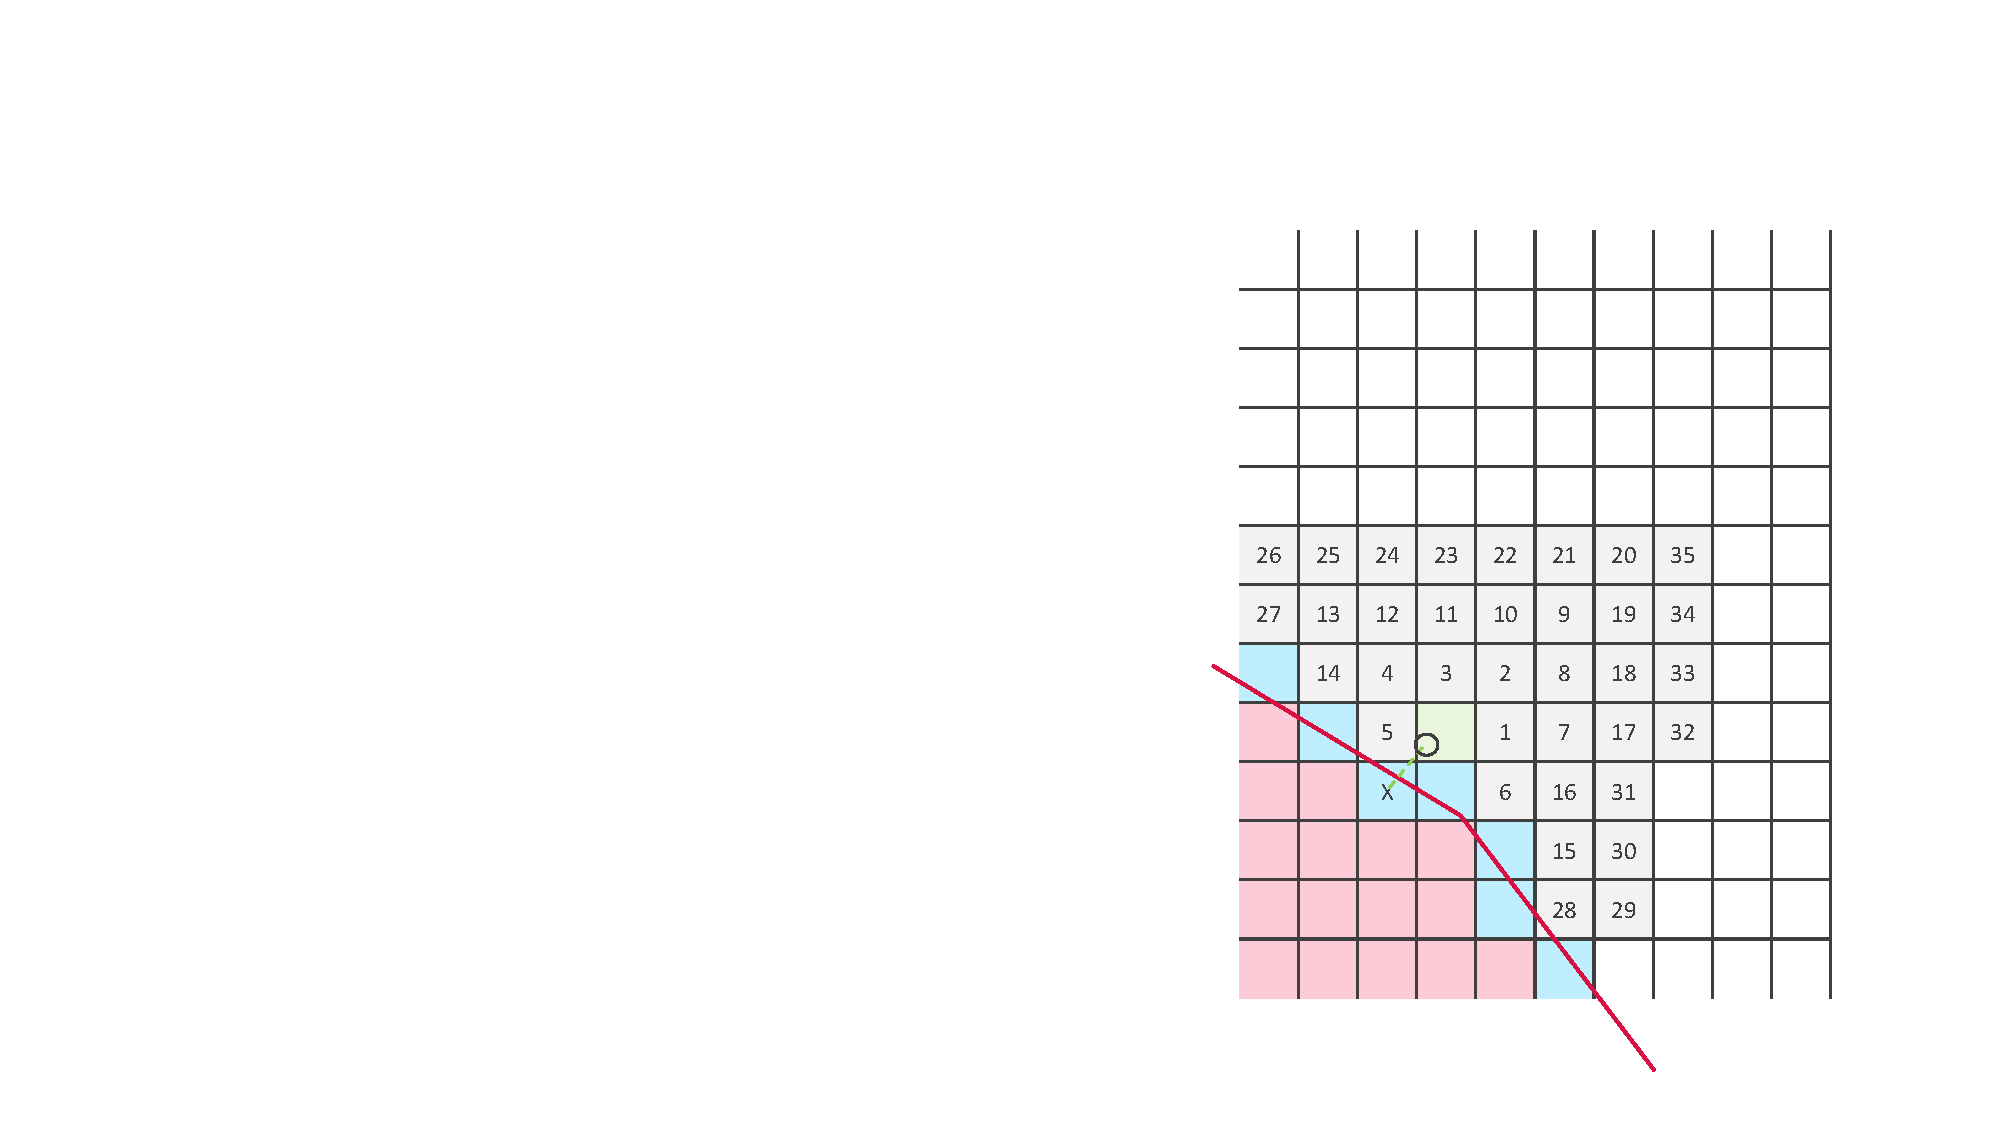
\includegraphics[width=0.35\linewidth]{chapter3_numerical_methods/pictures/BC_migrable1.pdf} &
        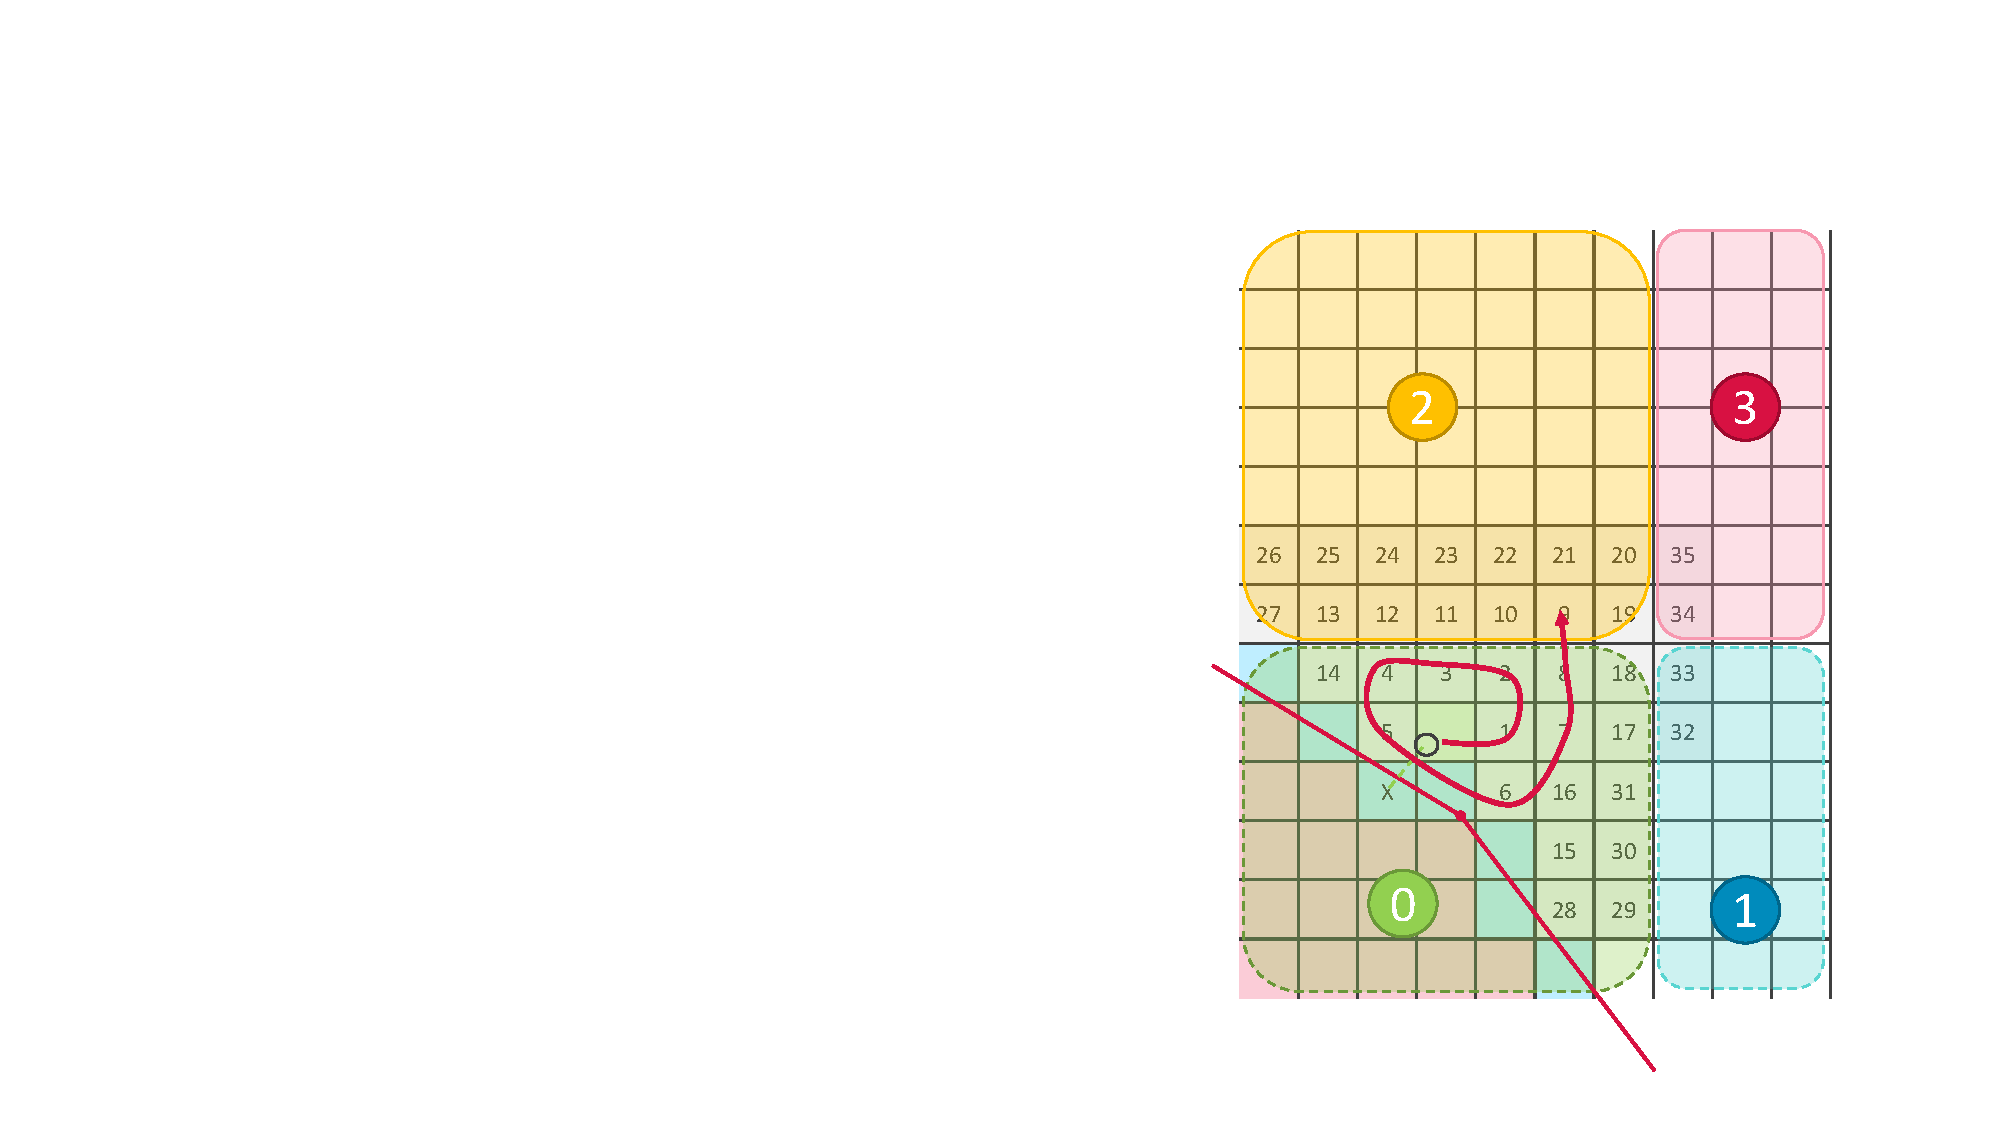
\includegraphics[width=0.35\linewidth]{chapter3_numerical_methods/pictures/BC_migrable2.pdf} \\ [0.5em]
        (a) & (b)
    \end{tabular}
    \caption{(a) Zoom on the neighborhood of an immersed boundary cell image and the corresponding surrounding cells numbering for the spiral walk.
    (b) Illustration of the spiral walk task in the migratable task algorithm and of the influence of partitioning thereupon - the halos are omitted as the algorithm does not make use of them.}
    \label{fig:migratable_task}
\end{figure}

To do so, we emit a probe that will march the surrounding cells in a spiral motion: for each "valid" neighbor (that is not an immersed cell), the index of the cell and the values of the fluid variables are stored in the probe structure before it goes on.
This marching is the \emph{task} in the migratable task paradigm - see figure~\ref{fig:migratable_task}(b) - which is supported by a simple data structure:

\begin{verbatim}
struct _probe_task_state
    status  // status of the marching
    (x,y,z) // current coordinate of the head of the probe

    coords[] // coordinates of valid neighbors, accumulated
    values[] // fluid variables in the valid neighbors, accumulated

    origin_rank // rank of the processes wherefrom the probe originates
    rank // rank of the process the probe needs to be sent to, if any

    count // current number of neighbors
end struct
\end{verbatim}

Because of the partitioning of the Cartesian mesh, several, if not all, processes own immersed boundary cells and must therefore emit probes.
In terms of implementation, each process has a stack of such tasks that it works through either sequentially or in parallel with multiple shared-memory OpenMP threads.
During its march, if a probe next step has to be taken on a different process (illustrated on figure~\ref{fig:migratable_task}(b)), then a message is sent from its current owner to the neighboring process containing the entire probe structure ; in so doing, the probe is popped from the previous owner stack of tasks and pushed to the neighbor process stack that can resume the walk of the probe.
This march of each probe continues until it has found enough valid neighbors, \emph{per} the user request, at which point the whole structure of the probe is sent back to the process it originated from so the least-square interpolation can take place and the immersed boundary cell can be populated with values enforcing the immersed boundary condition \cite{BRIDELBERTOMEU2021}.

Note that during the course of the algorithm, no process can predict with simple logic whether it is going to receive a task from a neighbor or whether it will have to send one of its tasks to a neighbor - since no process knows whether to expect a message, they all wait for messages asynchronously while handling the tasks on their stacks.
This poses a well-known problem in parallel computations, namely a termination issue.
Since no process knows to expect a message, if nothing is done all the processes will eventually finish working on their own tasks and wait indefinitely for messages from their neighbors.
To prevent such an infinite loop from occurring in HYPERION, we implemented the algorithm of Francez \emph{et al.} \cite{francez1982} to achieve distributed termination without introducing any new communication.

The entire pseudocode algorithm is described below.

\begin{verbatim}
while not terminated
    %MASTER THREAD
    {
        while to_send_stack not empty
            e := pop to_send_stack
            async send e to e.rank
            sent_stack push e
        end while
        while sent_stack not empty
            check sent request has gone through
        end while
        probe all sources for any message
        if message
            new_e := deserialize message
            stack push new_e
        end if
        terminated ?= francez termination algorithm
    }
    %END MASTER THREAD
    while stack not empty
        e := pop stack
        until enough neighbors
            go to the next cell in the spiral
            if next cell is solid or ghost
            then
                skip
            else
                if next cell on current process
                    e.coords append cell center coordinates
                    e.values append cell values
                    increment e.count
                    if enough neighbors
                        e.status := SUCCESS
                        break until
                    end if
                else
                    e.rank := neighbor rank
                    break until
                end if
            end if
        end until
        if e.status == SUCCESS
            e.rank := e.origin_rank
        end if
        if e.status == SUCCESS and current process rank == e.origin_rank
            solve least square problem
            compute immersed ghost cell value
        else
            to_send_stack push e
        end if
    end while
end do
\end{verbatim}

This migratable task strategy allowed us to use the ENO-like interpolation algorithm with large neighborhoods in massively parallel computations with guaranteed stability, yielding a satisfactory speed-up up to $4096$ processes as shown on figure~\ref{fig:speed_up}.

\begin{figure}
    \centering
    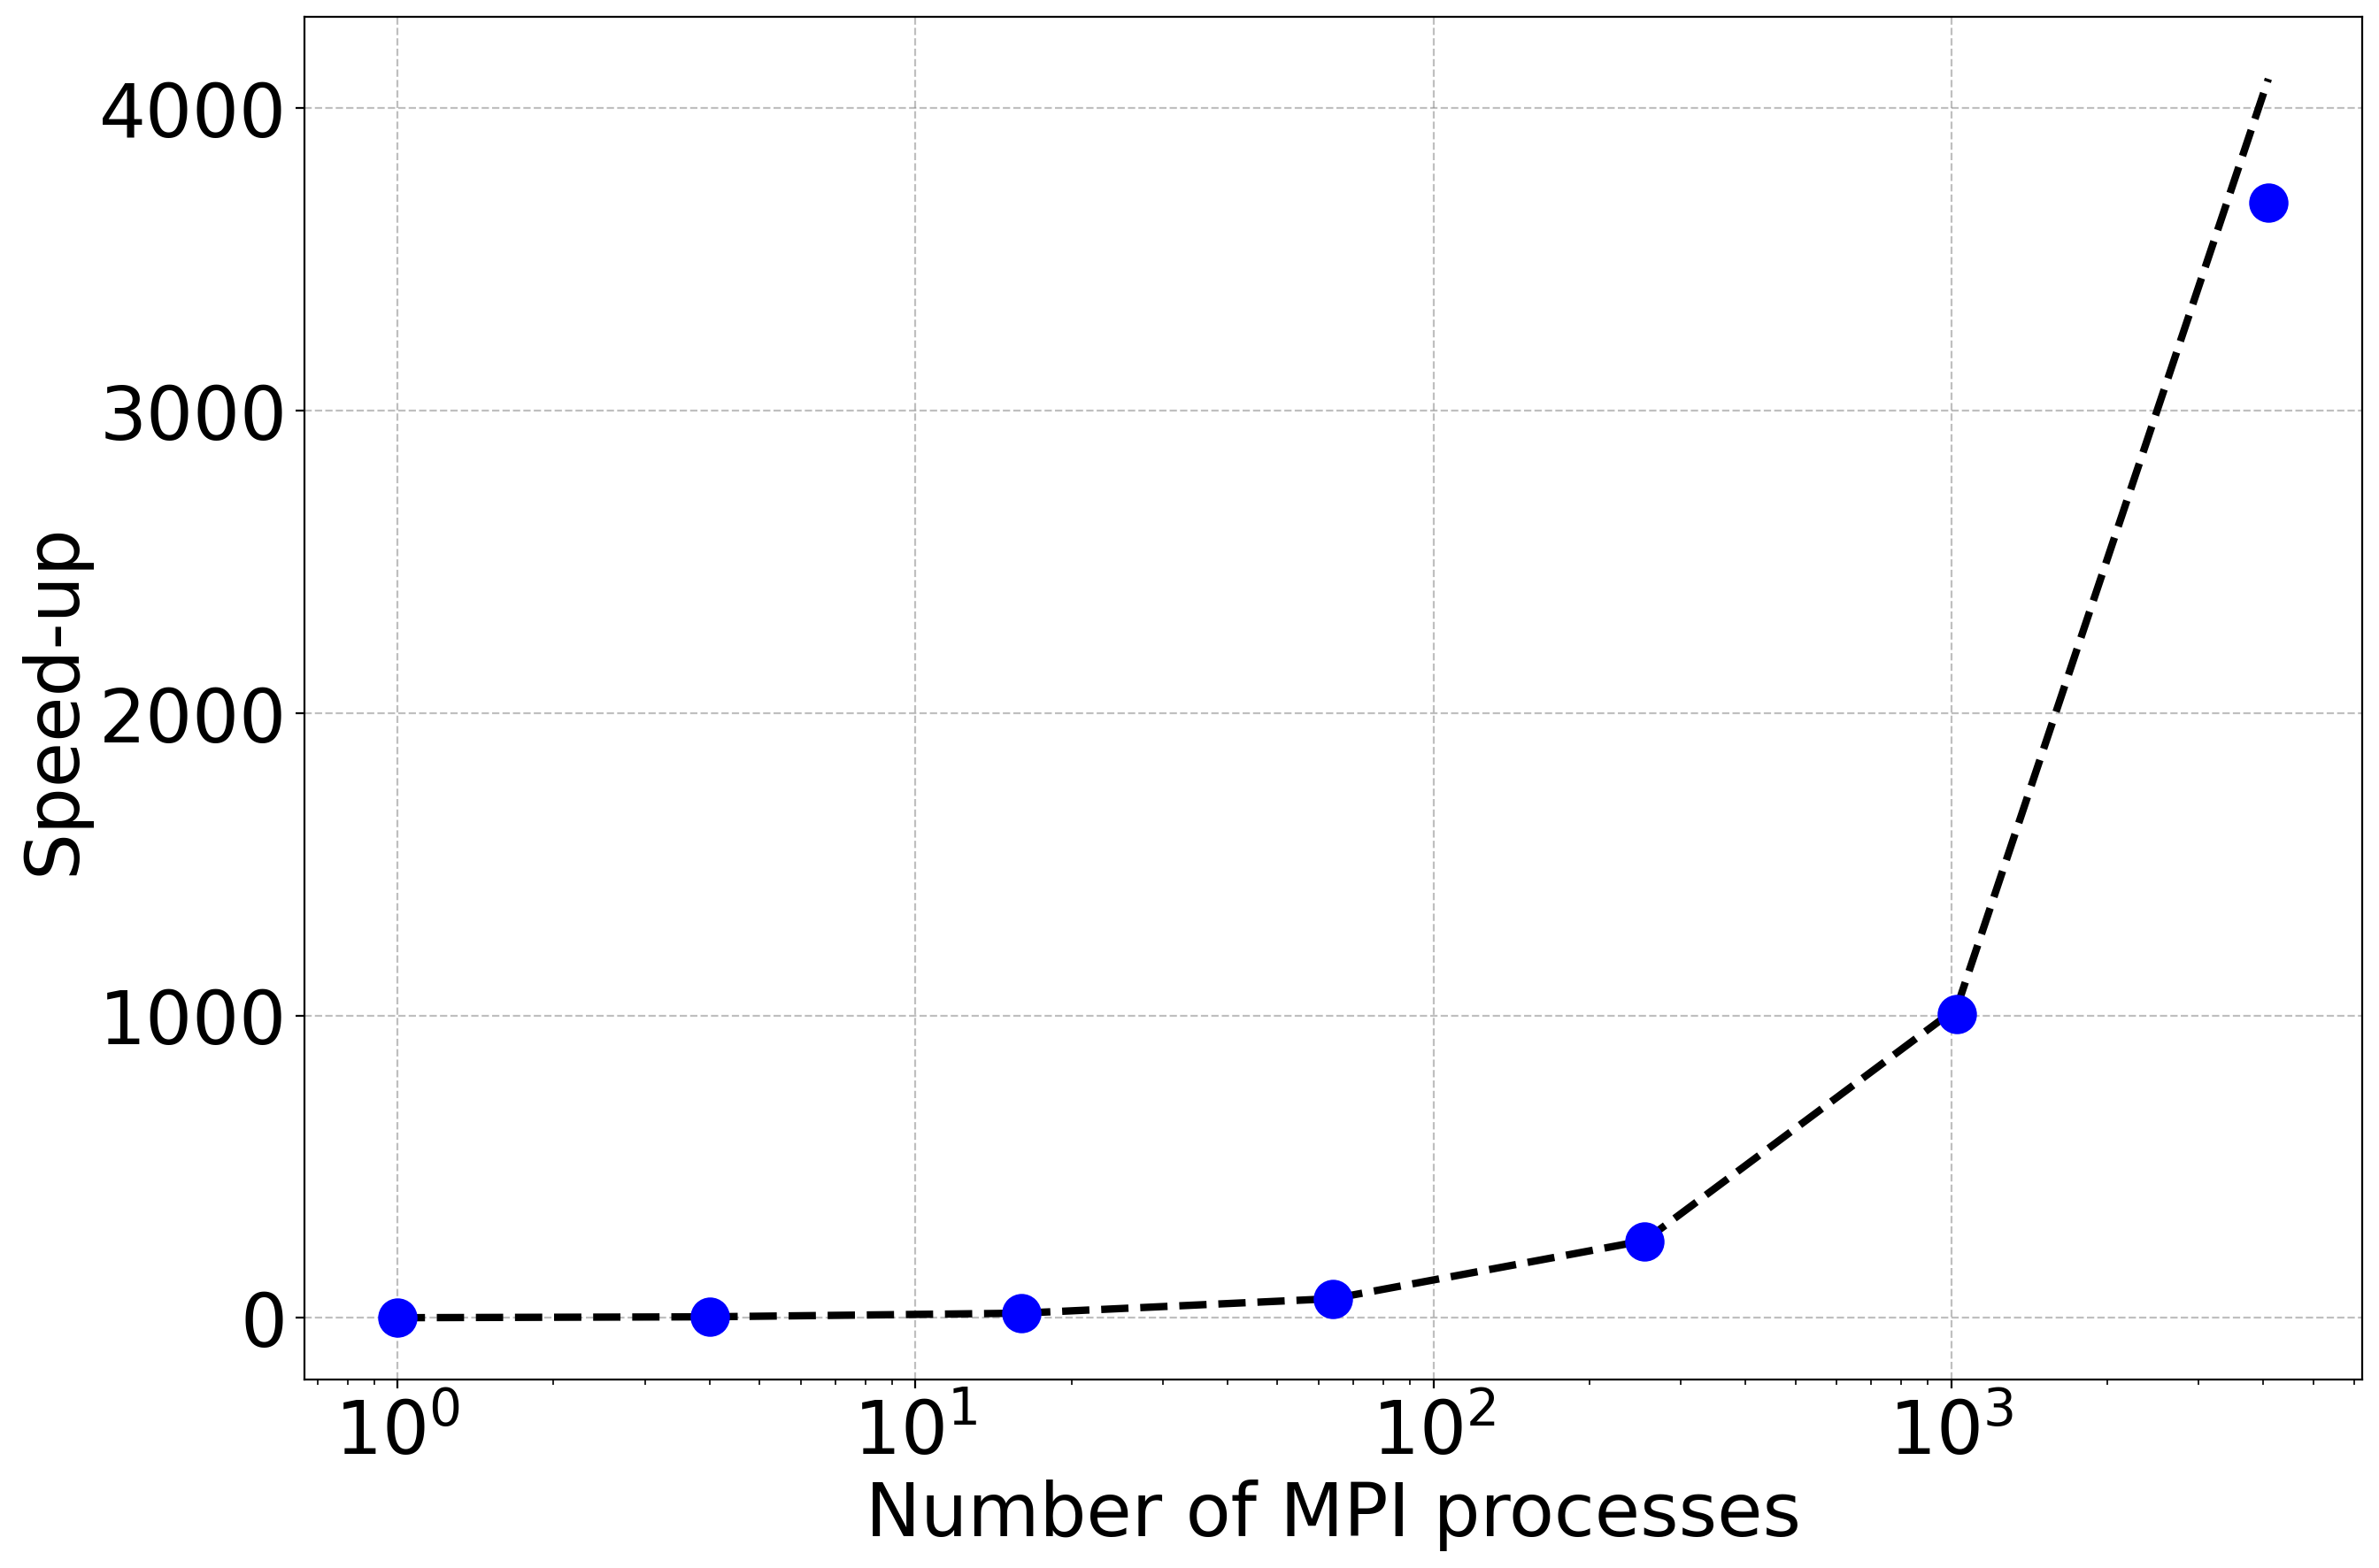
\includegraphics[width=0.75\linewidth]{chapter3_numerical_methods/pictures/speed_up.png}
    \caption{Speed up achieved for distributed parallelism with HYPERION and the migratable task algorithm - ideal speed-up (dashed line) versus actual speed-up (blue dots).
    Data collected for a single immersed body using AMD Rome processors.}
    \label{fig:speed_up}
\end{figure}

%
% [TBB] Ici c'est peut-être le plus délicat.
% On veut pas faire non plus un papier de HPC, donc on peut pas se permettre de rentrer dans tous les détails hyper techniques.
% Mais c'est quand même ECCOMAS, donc il faut pas non plus qu'on ait pas l'air de maîtriser le sujet....
% Je pense qu'on peut découper cette partie en plusieurs sous-parties qui racontent comment on est arrivé au besoin & à l'écriture
% de l'algo avec des tâches migrables
% + Comment ça marche en séquentiel (let's say shared-memory rather than purely sequential, that allows us to immediately include OpenMP considerations), en gros c'est quoi l'algo et comment on relie la taille/longueur/compléxité de la recherche de voisins à l'ordre (en gros cf C&F 2021)
% + Si on utilise une approche classique distribuée où en gros on s'appuie que sur des halos, ça donnerait quoi en terme de taille de halos, en terme de Gb communiqués etc ... -- ça expliquera bien pourquoi il faut faire quelque chose.
% + Notre proposition d'algo distribué basé sur des tâches migrables
%   + Faudra rapidement évoquer la structure de données en liste chaînée pour le traitement contigu des tâches sur un process MPI
%   + On parle de comment la migration se passe : comme les processes ne savent pas forcément s'ils vont recevoir un message, ils doivent attendre indéfiniment
%   + Du coup on a un problème de complétion -- it's quite easy to know if, locally, we still have tasks to accomplish, but it's very hard to know whether another process might send a task ==> we need a consensus algorithm, and there is actually one in the paper by Francez that we can use
% + On oubliera pas de mettre des morceaux de pseudo-code un peu partout pour soutenir notre argumentation -- je ne pense pas qu'il faille prendre le temps d'écrire suffisamment pour que ça soit reproductible par n'importe qui, mais il faut au moins donner suffisamment de détails pour que ça paraisse effectivement faisable
% + Et il va falloir sortir des cas tests aussi à ce moment là ... alors là c'est pas évident non plus parce que la version de l'algo "avec halo" n'existe plus nul part donc il va falloir truander ... à voir !
%

\section{TOWARDS HIGH-FIDELITY SIMULATIONS}\label{sec:high_fidelity}
%
% [TBB] Alors maintenant qu'on a raconté tout ce qu'on a raconté au dessus, il faut absolument mettre l'accent
% sur le fait que ça a rendu possible les simulations 3D à des coûts raisonnables et que sans ces deux optimisations on
% pouvait pas vraiment envisager du 3D massivement parallèle avec IBC.
% Du coup maintenant qu'on a ça, on peut se concentrer sur la LES pour améliorer un peu la fidélité physique d'HYPERION quand
% les maillages ne sont pas DNS-like.
% + On peut mentionner rapidement la légère modification des équations de NS quand on arrive dans le monde de la LES : ajout
% d'une notion de viscosité turbulente à la Boussinesq via un modèle de sous-maille (on a aussi un Prandtl turbulent qui fait
% son apparition du coup)
% + On peut parler des ambitions d'ajout de loi de paroi - on est pas forcé d'avoir des résultats je pense si on mentionne bien
% qu'il s'agit d'un travail de doctorat en cours, mais il faudrait peut-être déjà donner des billes sur comment on pense faire
% et où on aimerait brancher ça.
% + Attention quand même à ce dernier point ... publier des choses comme ça, en avance de phase et sans résultats, ça peut aussi
% conduire à ce qu'une autre équipe y arrive avant nous et le publie - il faut qu'on détermine jusqu'où on avance nos pions.
%

The two algorithms/strategies presented in sections~\ref{sec:rasterization} and~\ref{sec:migratable_tasks} made possible running massively parallel simulations in three dimensions with HYPERION: before the introduction of the former, detecting solid cells on realistic meshes of the order of $10^8$ cells would take several days, and before the introduction of the latter, three-dimensional computations with immersed objects would be too expensive and, most often, would fail altogether during the spiral walks.
In the high Mach and Reynolds numbers regimes where this study places itself, direct numerical simulations (DNS) are out of reach because of their prohibitive computational cost.
However, we aim at running large eddy simulations (LES) with an \emph{ad hoc} subgrid-scale model to improve the predictive capabilities of HYPERION in the compressible regime even on coarse meshes - gaining the ability to run three-dimensional simulations was a first step in that direction.

An in-depth presentation of the LES equations for compressible flows is out of the scope of this paper (the interested reader is referred \emph{e.g.} to Garnier \emph{et al.} \cite{Garnier2009}), but recall that solving the LES equations implies using a filtered version of the compressible Navier-Stokes equations~\eqref{eq:cons_ns}-\eqref{eq:cons_ns_vectors}, among which the momentum equations now read:

\begin{equation}
    \dfrac{\partial \bar\rho \tilde{u}_i}{\partial t} + \dfrac{\partial \bar\rho \tilde{u}_i\tilde{u}_j}{\partial x_j} + \dfrac{\partial \bar p}{\partial x_i} - \dfrac{\partial \overset{\smile}{\sigma}_{ij}}{\partial x_j} = -\dfrac{\partial \tau_{ij}}{\partial x_j} + \dfrac{\partial}{\partial x_j} \left( \overline{\sigma_{ij}} - \overset{\smile}{\sigma}_{ij}\right),
    \label{eq:les_momentum_eqns}
\end{equation}

where the $\tilde{\cdot}$ overset denotes Favre averaging, the $\bar\cdot$ overset denotes Reynolds averaging, and $\overset{\smile}{\sigma}_{ij}$ depends on the computable rate-of-strain tensor:

\begin{equation}
    \overset{\smile}{\sigma}_{ij} = \mu(\tilde{T}) \left( 2 \tilde{S}_{ij} - \dfrac{2}{3}\delta_{ij}\tilde{S}_{kk} \right),~~ \tilde{S}_{ij} = \dfrac{1}{2}\left( \dfrac{\partial\tilde{u}_i}{\partial x_j} + \dfrac{\partial \tilde{u}_j}{\partial x_i}\right).
    \label{eq:sigma_smile}
\end{equation}

All overset variables are computable whereas we need a closure for the subgrid-scale stress tensor $\tau_{ij}$.
In HYPERION, we follow a Boussinesq type hypothesis \cite{boussinesq1877essai} that leads to the subgrid-scale stress tensor having the following mathematical form:

\begin{equation}
    \tau_{ij} - \dfrac{1}{3}\delta_{ij}\tau_{kk} = - 2 \bar\rho \nu_{\text{sgs}} \left( \tilde{S}_{ij} - \dfrac{1}{3} \delta_{ij}\tilde{S}_{kk} \right),
    \label{eq:boussinesq_les}
\end{equation}

where $\nu_{\text{sgs}}$ represents a scalar subgrid viscosity that is left to be modelled.
In the present study we rely on the Wall-Adapting Local Eddy-viscosity model (WALE) by Ducros \emph{et al.} \cite{ducros1998wall} to run preliminary tests with the LES version of HYPERION.

\subsection{Taylor-Green Vortex}\label{ssec:test_tgv}

Before trying to evaluate the quality of the LES computations in the presence of immersed obstacles, let us run a very classical viscous test case that will allow us to check the implementation of the WALE model.

We are therefore considering the case of a Taylor-Green vortex which set-up and reference solution can be obtained from the 3$^{\text{rd}}$ international workshop on higher-order CFD methods \cite{diosady2015case}.
The domain is a periodic cube of dimensions $[-\pi, \pi]^3$, and the initial solution is given by the following expressions:

\begin{equation}
    \left\lbrace
    \begin{array}{ccl}
        u &=& \sin{\left( x \right)} \cos{ \left( y \right) } \cos{ \left( z \right) }, \\[0.6em]
        v &=& -\cos{\left( x \right)} \sin{ \left( y \right) } \cos{ \left( z \right) }, \\[0.6em]
        w &=& 0, \\[0.6em]
        p &=& \dfrac{1}{\gamma M_{\infty}^2} + \dfrac{1}{16}\left( \cos(2 x) + \cos(2 y) \right) \left( \cos(2 z) + 2\right), \\[0.6em]
        \rho &=& \gamma M_{\infty}^2 p.
    \end{array}
    \right.
\end{equation}

In this problem, we do not intend to validate in any way the behavior of the immersed boundaries algorithms.
Rather, we shall inspect the temporal evolution of the kinetic energy $E_k$ and of the enstrophy $\varepsilon$ integrated over the domain and compare it to the reference solution \cite{diosady2015case}.
Note that the mathematical expression used in this study for the kinetic energy is:

\begin{equation}
    E_k = \dfrac{1}{N^3} \sum_{i,j,k} \dfrac{1}{2} \rho_{i,j,k} \left(u_{i,j,k}^2 + v_{i,j,k}^2 + w_{i,j,k}^2\right),
    \label{eq:kinetic_eqn}
\end{equation}

and that of the enstrophy is:

\begin{equation}
    \epsilon = \dfrac{1}{N^3}\sum_{i,j,k} \dfrac{1}{2} \rho_{i,j,k} \left( \omega_{x; i,j,k}^2 + \omega_{y; i,j,k}^2 + \omega_{z; i,j,k}^2 \right),
    \label{eq:enstrophy}
\end{equation}

where $N$ stands for the number of cells along one side of the domain (assuming the Cartesian mesh is homogeneous), and $\mathbf{\omega} = \nabla \times \mathbf{u}$ is the vorticity.
To observe the convergence of the solution towards the reference solution, computations results on meshes of sizes $64^3$ and $512^3$ are shown here.
The computations were furthermore run using the AUSM$^+$-up Riemann solver in conjunction with the fifth-order TENO reconstruction scheme.

\begin{figure}[ht!]
    \centering
    \begin{tabular}{cc}
        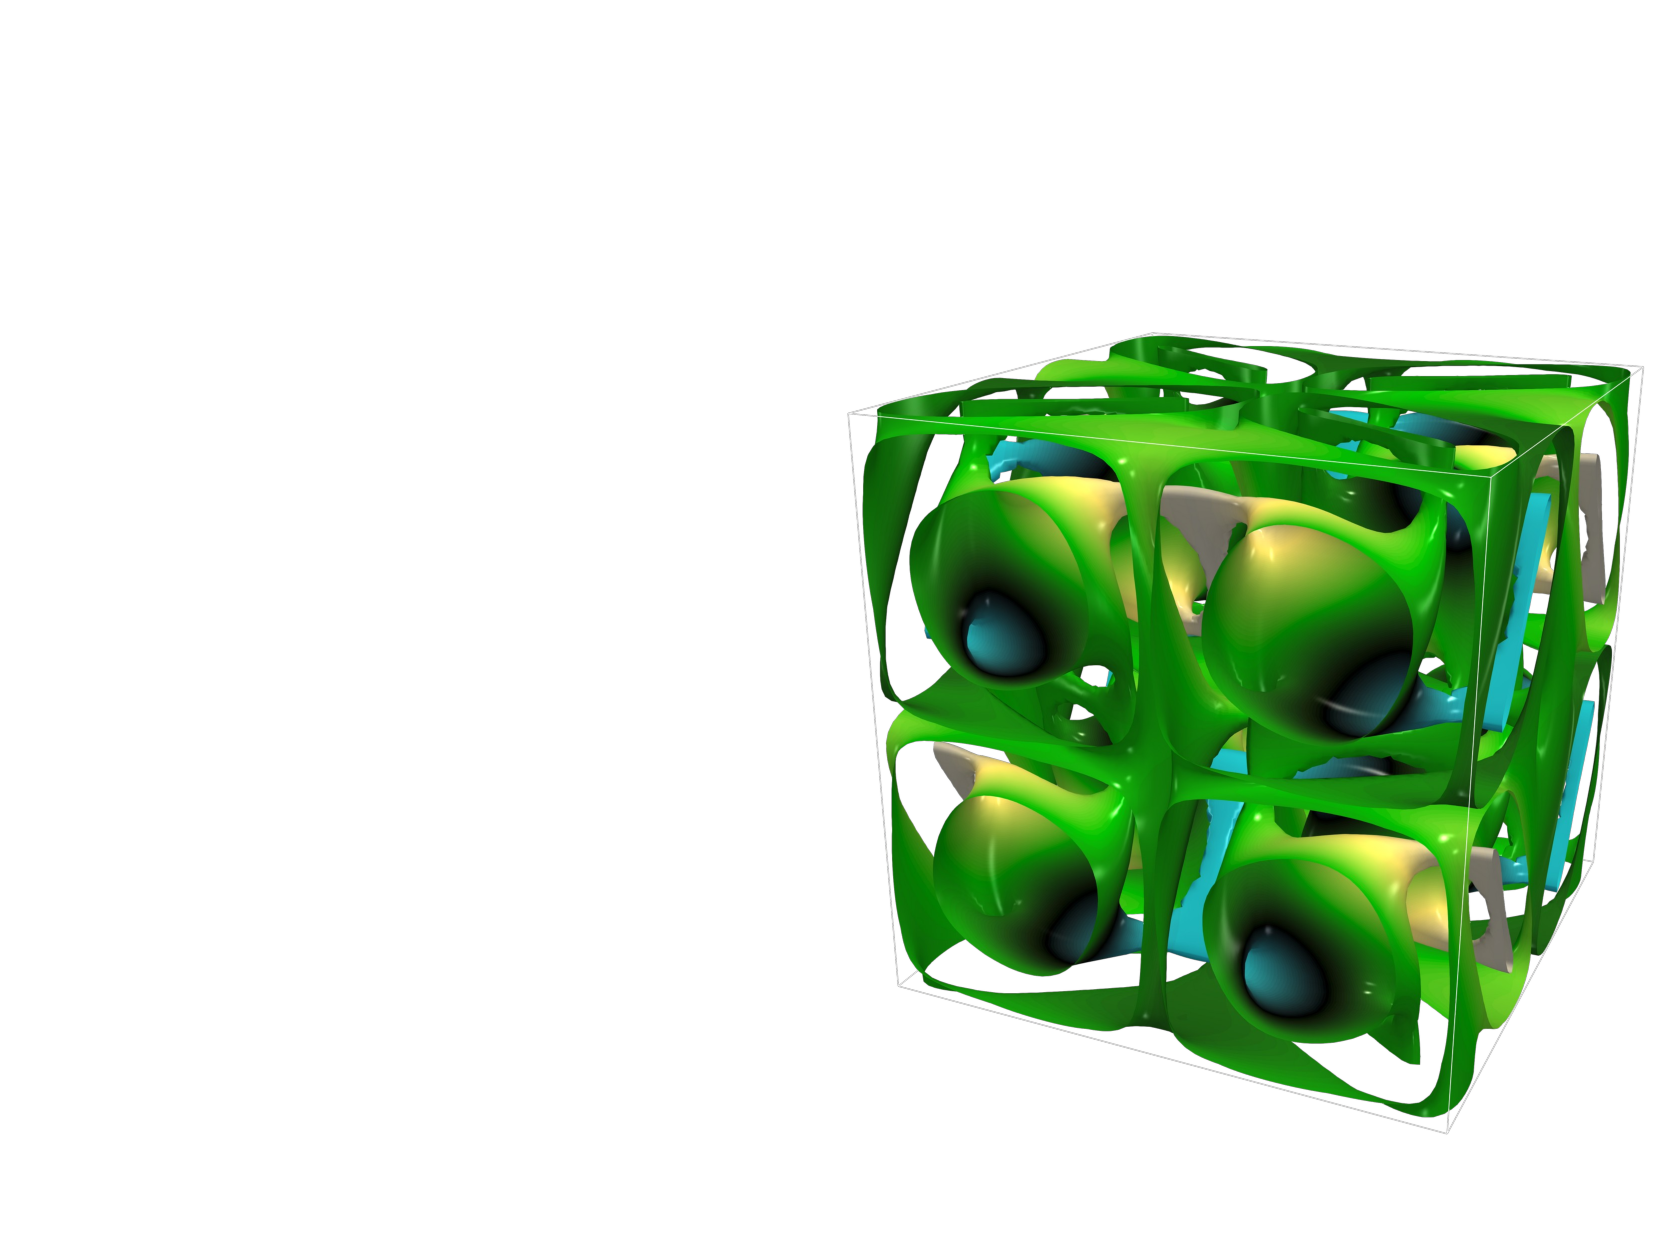
\includegraphics[width=0.45\linewidth]{chapter3_numerical_methods/pictures/TGV_coarse.pdf} &
        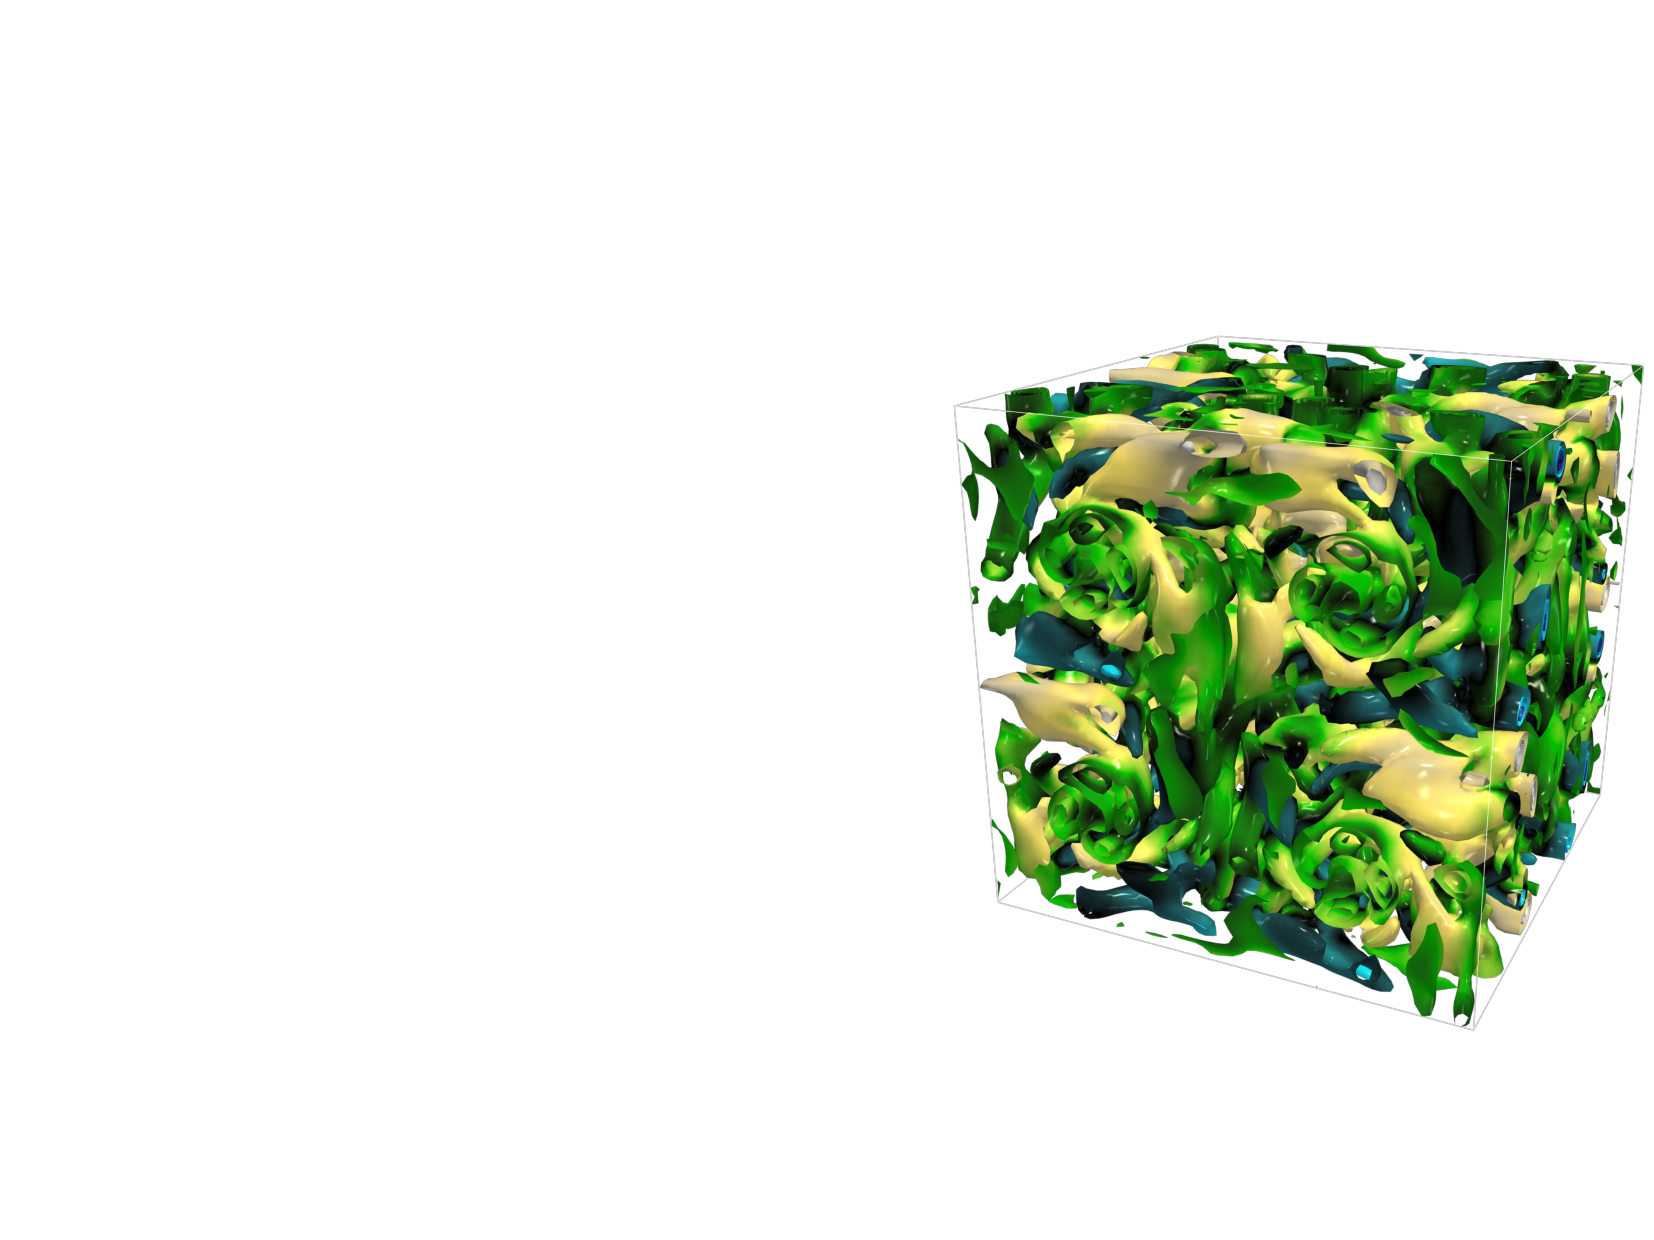
\includegraphics[width=0.45\linewidth]{chapter3_numerical_methods/pictures/TGV_fine.pdf} \\
        (a) & (b)
    \end{tabular}
    % \caption{Snapshot of the state of the Taylor-Green vortex after $20$ characteristic times, (a) on the $64^3$ mesh and (b) on the $512^3$ mesh.
    % Isocontours of the Q-criterion are represented, colored by the norm of the vorticity.}
    \caption{Snapshots of the state of the Taylor-Green vortex after (a) $1$ characteristic time and (b) $20$ characteristic times on the $64^3$ mesh.
    Isocontours of enstrophy are represented, colored by the magnitude of velocity.}
    \label{fig:TGV_view}
\end{figure}

Figure~\ref{fig:TGV_view} presents the three-dimensional structures present in both the coarse and the fine flow as isocontours of the Q-criterion colored by the magnitude of the vorticity.
As expected, the turbulence is allowed to develop itself down to much smaller scales on the fine mesh.

\begin{figure}[ht!]
    \centering
    \begin{tabular}{cc}
        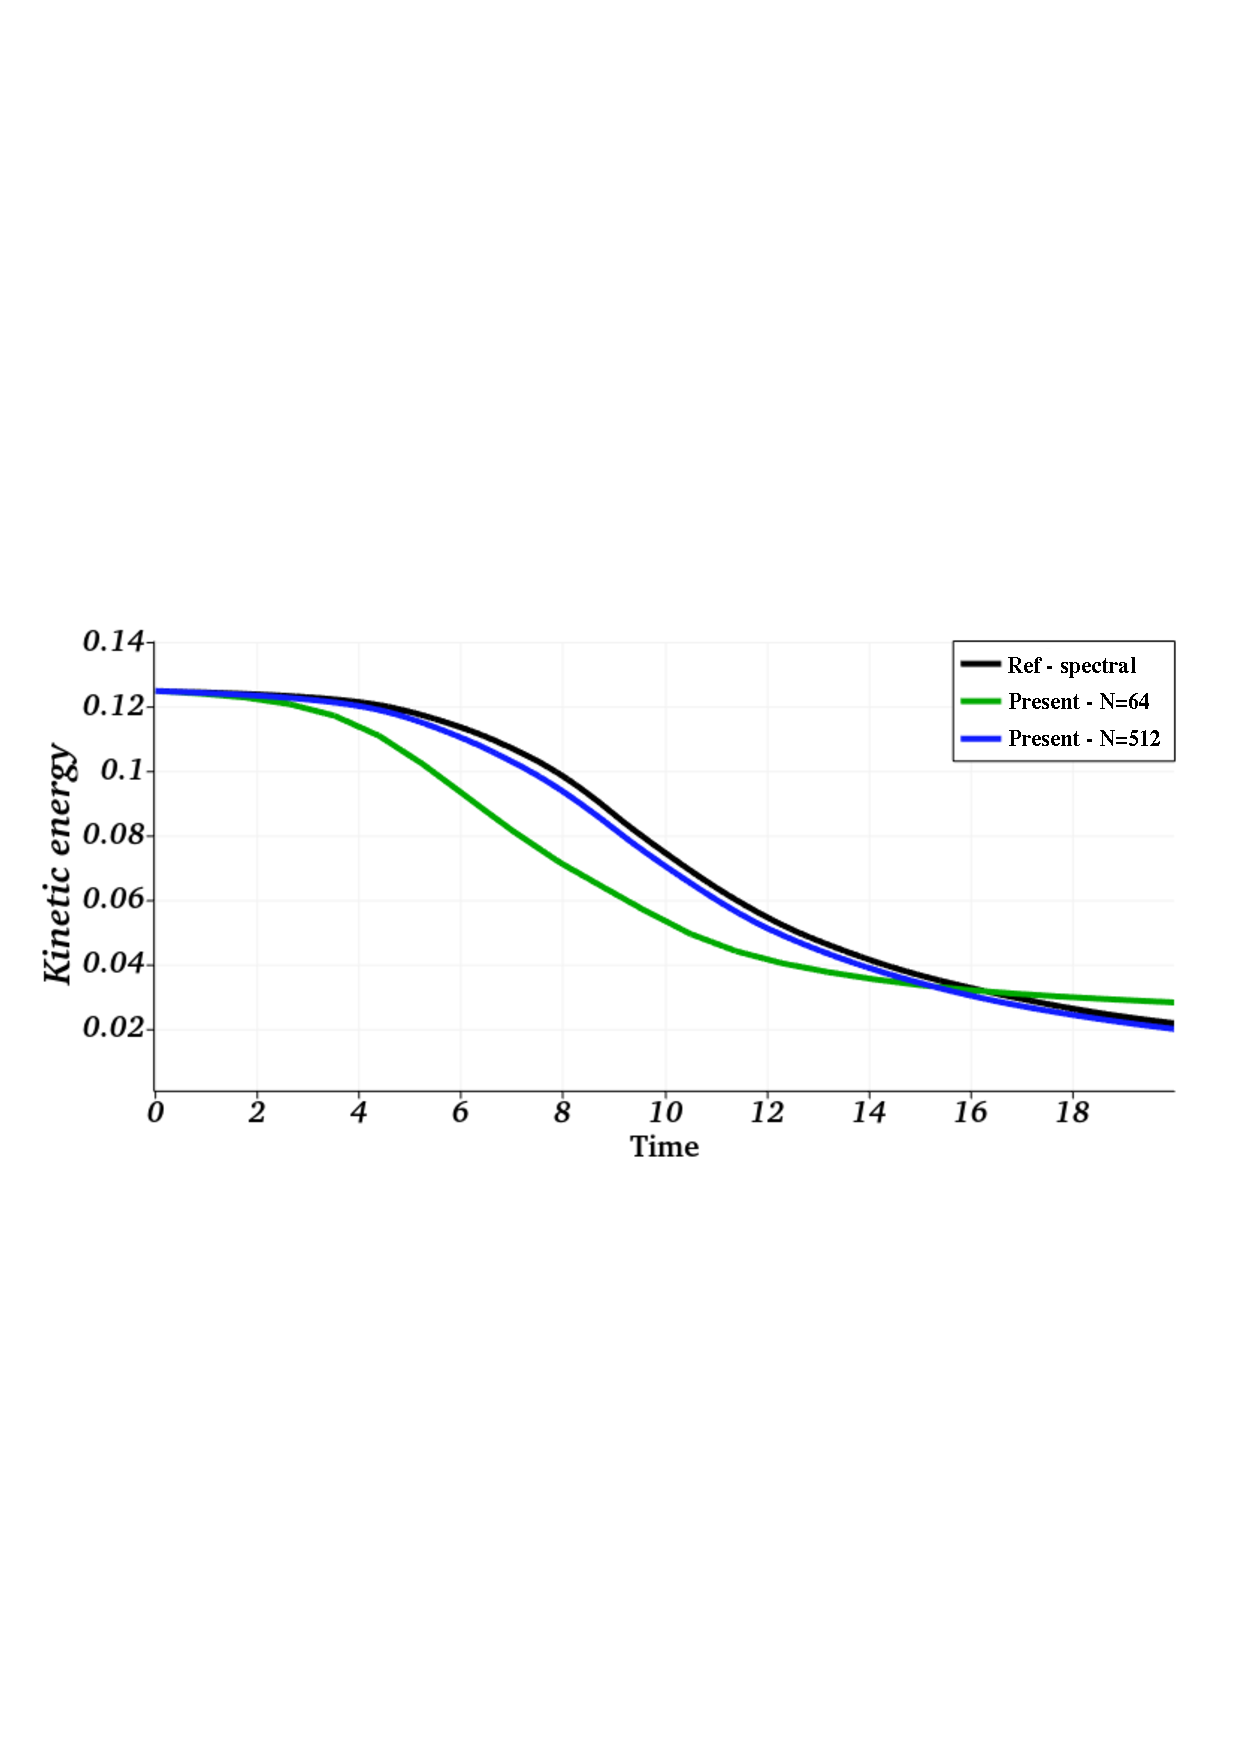
\includegraphics[width=0.47\linewidth]{chapter3_numerical_methods/pictures/TGV_energy_v2.pdf} &
        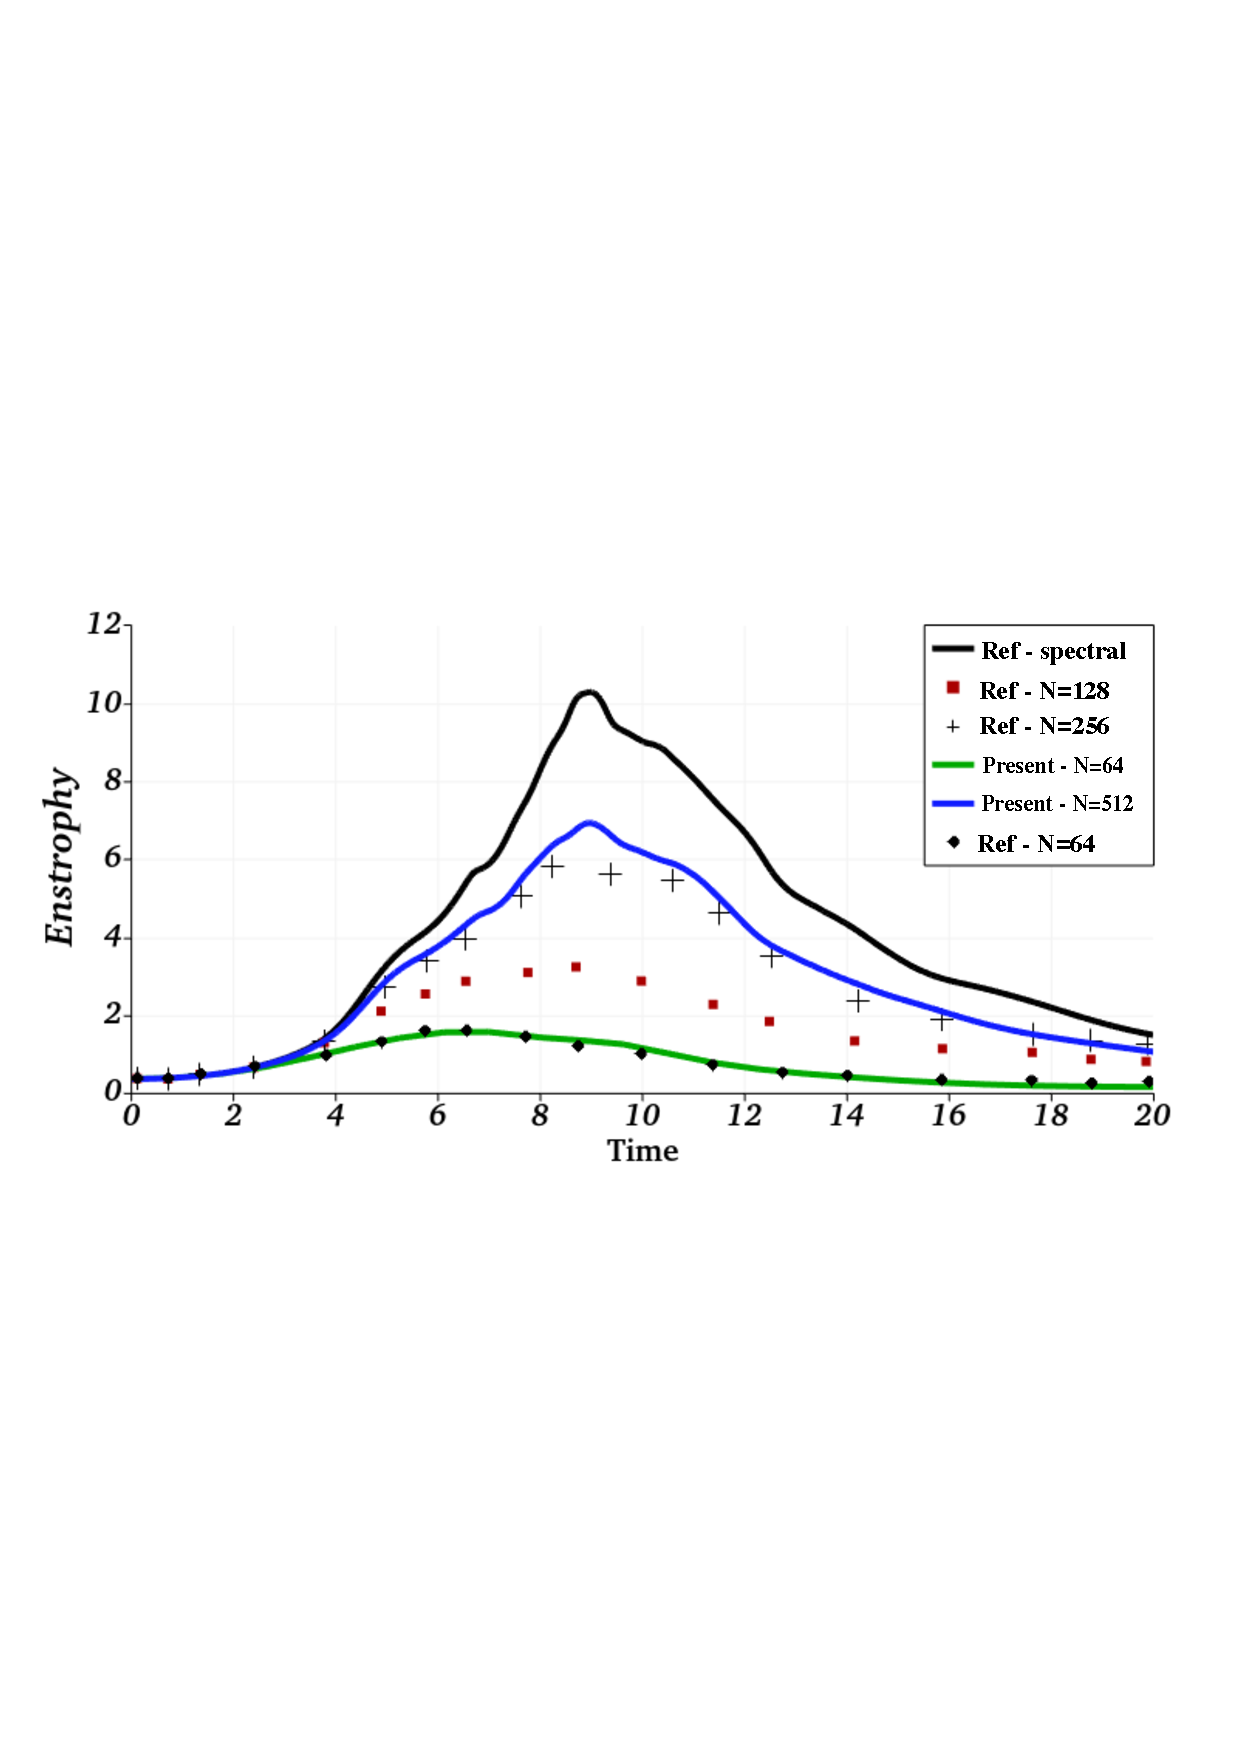
\includegraphics[width=0.47\linewidth]{chapter3_numerical_methods/pictures/TGV_enstrophy_v2.pdf} \\
        (a) & (b)
    \end{tabular}
    \caption{Comparison of the temporal evolution of (a) the kinetic energy (see equation~\eqref{eq:kinetic_eqn}) and (b) the enstrophy (see equation~\eqref{eq:enstrophy}) against the $512^3$ spectral computation from \cite{diosady2015case} (black line) and the high-order computations from \cite{giangaspero2015case} (symbols).}
    \label{fig:TGV_comparison}
\end{figure}

Figure~\ref{fig:TGV_comparison} introduces a more quantitative comparison between the present results and both the reference spectral computation conducted on a $512^3$ mesh in \cite{diosady2015case} and some high-order reference computations from \cite{giangaspero2015case}.
The results are satisfactory and show the convergence towards the reference for both metrics - the kinetic energy, figure~\ref{fig:TGV_comparison}(a) and the enstrophy, figure~\ref{fig:TGV_comparison}(b).
The results in terms of enstrophy seem further away but in another exhaustive study (unpublished yet) the authors show the prime importance of the approximate Riemann solver on the quality of the enstrophy production in a finite-volume code, and although the AUSM$^+$-up solver is particularly adapted at handling all-speed flows with hypersonic regions, it might not be the ideal solver for fine turbulence behavior - such a discussion is however out of the scope of this paper.

\subsection{Double cone}\label{ssec:test_double_cone}

With the implementation of the subgrid-scale model validated by the turbulence testcase discussed in paragraph~\ref{ssec:test_tgv}, we move on to the study of the flow around two documented configurations in supersonic or hypersonic regimes.

\begin{figure}[ht!]
    \centering
    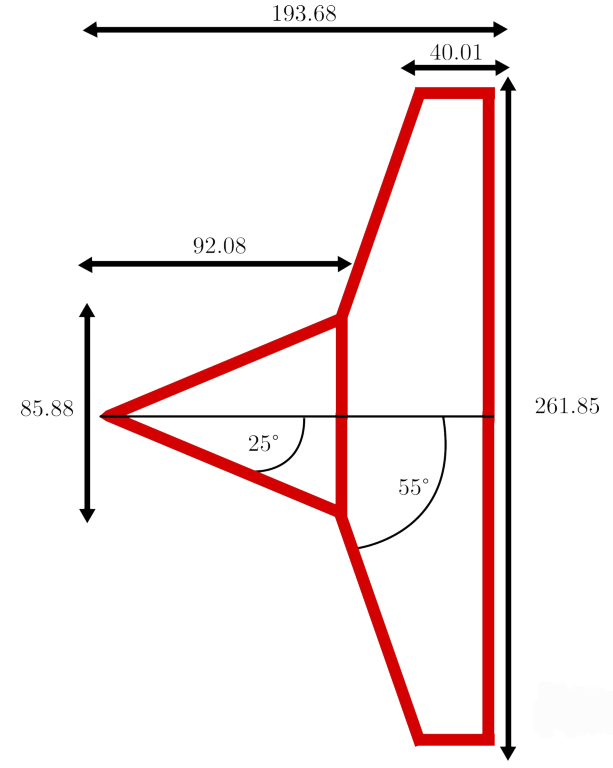
\includegraphics[width=0.40\linewidth]{chapter3_numerical_methods/pictures/double_cone.pdf}
    \caption{Geometrical details of the double-cone configuration.}
    \label{fig:double_cone_geom}
\end{figure}

For the first immersed boundary condition testcase, the hypersonic flow over an axisymmetric double cone configuration (see figure~\ref{fig:double_cone_geom}) is studied at Mach number $12.2$ and Reynolds number $14 \times 10^6$.
The wall temperature is fixed at $1.75T_{\infty}$.
The results presented below correspond to meshes made of $1,200,000$ and $4,000,000$ cells, qualified of coarse and fine, respectively (as it is an axisymmetric obstacle, the simulation itself has been treated as a two-dimensional, axisymmetric simulation).

A qualitative visualization of the resulting flow is provided on figure~\ref{fig:double_cone_schlieren} in the form of a numerical Schlieren image.
It mostly shows the regions where strong changes in density occur, allowing the user to visualize the shock and contact waves, and, like in the present case, the boundary layer developing along the wall.
An inset has been added to the figure to put the light on the lambda-shock pattern found after the boundary layer passes the recirculation region and reattaches itself to the wall of the second cone.

\begin{figure}[ht!]
    \centering
    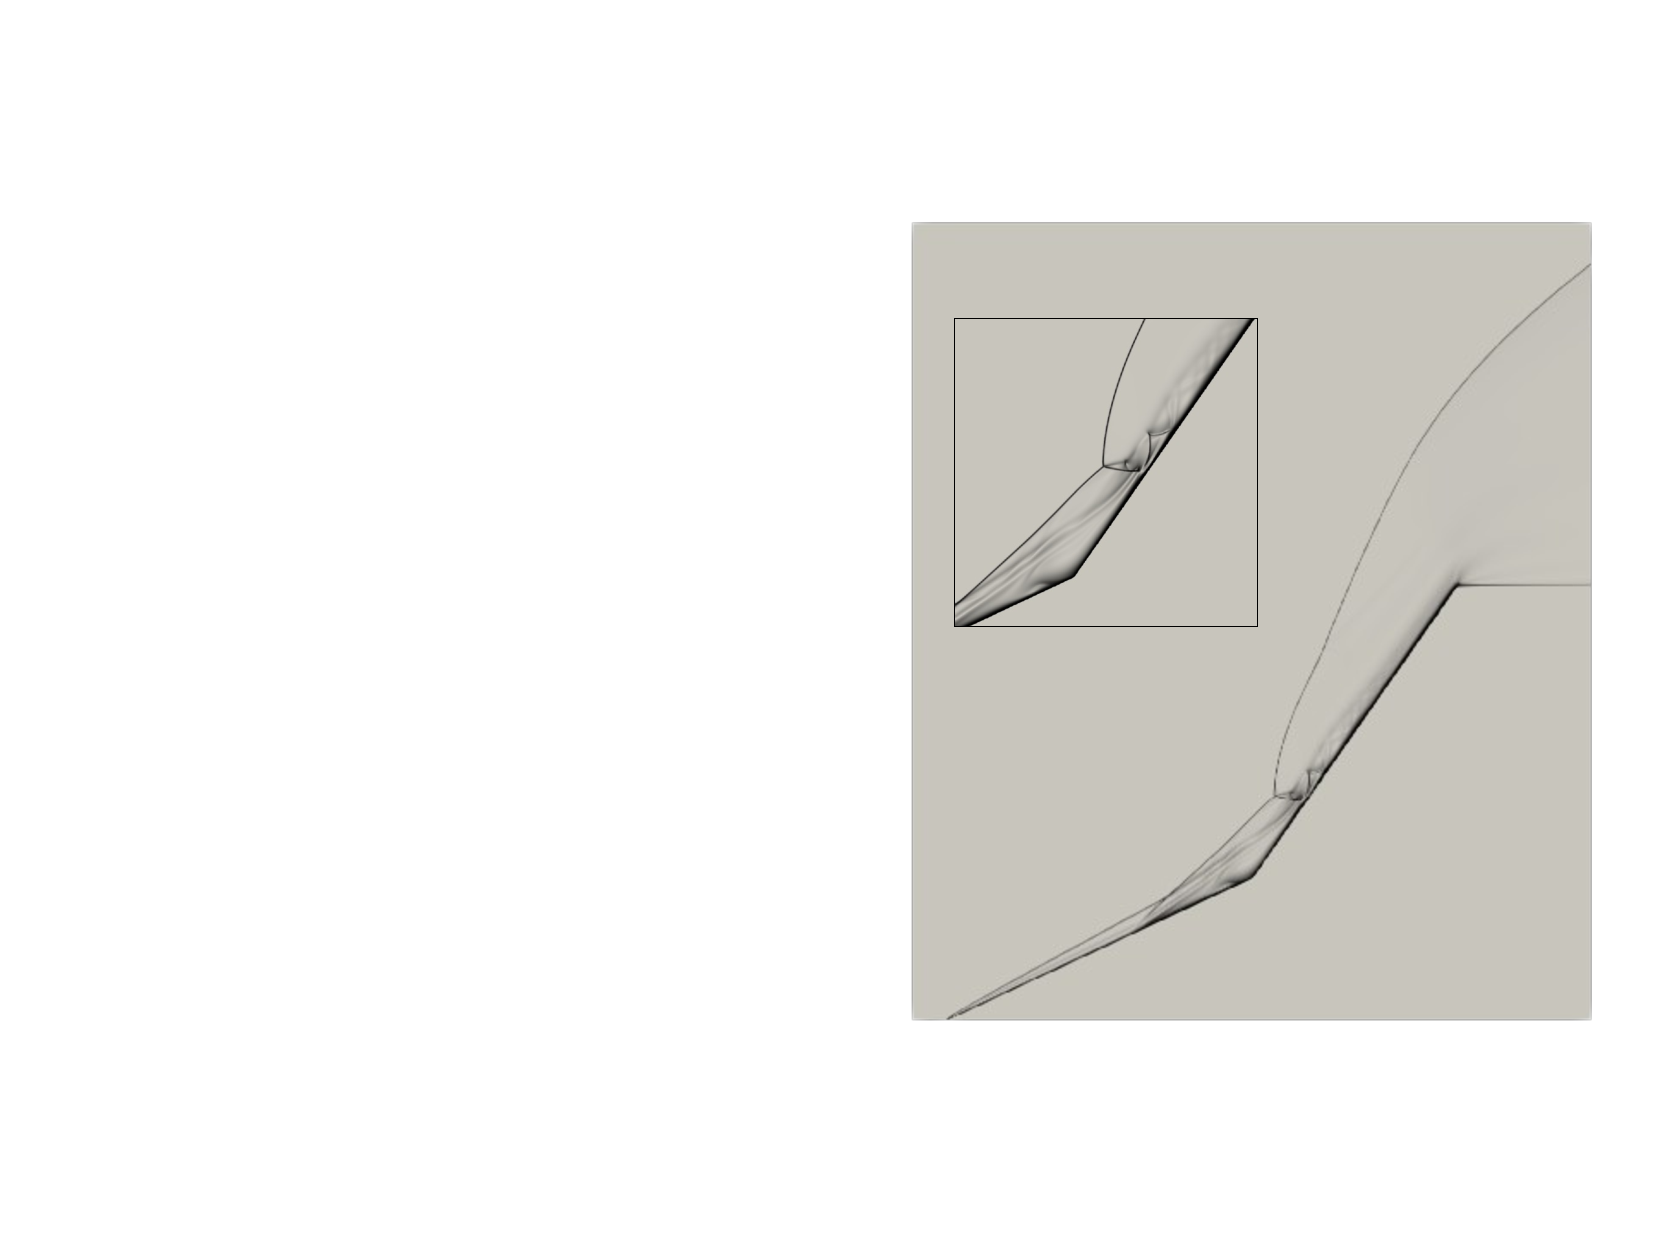
\includegraphics[width=0.35\linewidth]{chapter3_numerical_methods/pictures/double_cone_schlieren.pdf}
    \caption{Numerical Schlieren imaging of the flow around the double cone configuration.
    The inset zooms in on the lambda-shock pattern found after the recirculation region at the change of wall angle.}
    \label{fig:double_cone_schlieren}
\end{figure}

In a more quantitative manner, the wall pressure and the wall heat flux are compared against the experimental results obtained by MacLean \emph{et al.} \cite{MacLean2014} - see figure~\ref{fig:double_cone_comp}(a) and (b).
Without much effort, the wall pressure is correctly predicted - figure~\ref{fig:double_cone_comp}(a) - because it is mostly driven by the inviscid behavior of the simulation and does not depend too much on the resolution of the near-wall flow.
In contrast, the viscous heat flux is not as well predicted because boundary layers are not resolved properly with the immersed boundary method implemented in HYPERION.
Even with a fine mesh, although the peak of heat flux is correctly captured both in terms of coordinates and magnitude, the heat flux levels after the reattachment of the boundary layer are markedly underestimated.
This is a well known shortcoming of any immersed boundary method, and a future study will be dedicated to correcting it with the help of \emph{ad hoc} wall laws.

\begin{figure}[ht!]
    \centering
    \begin{tabular}{cc}
        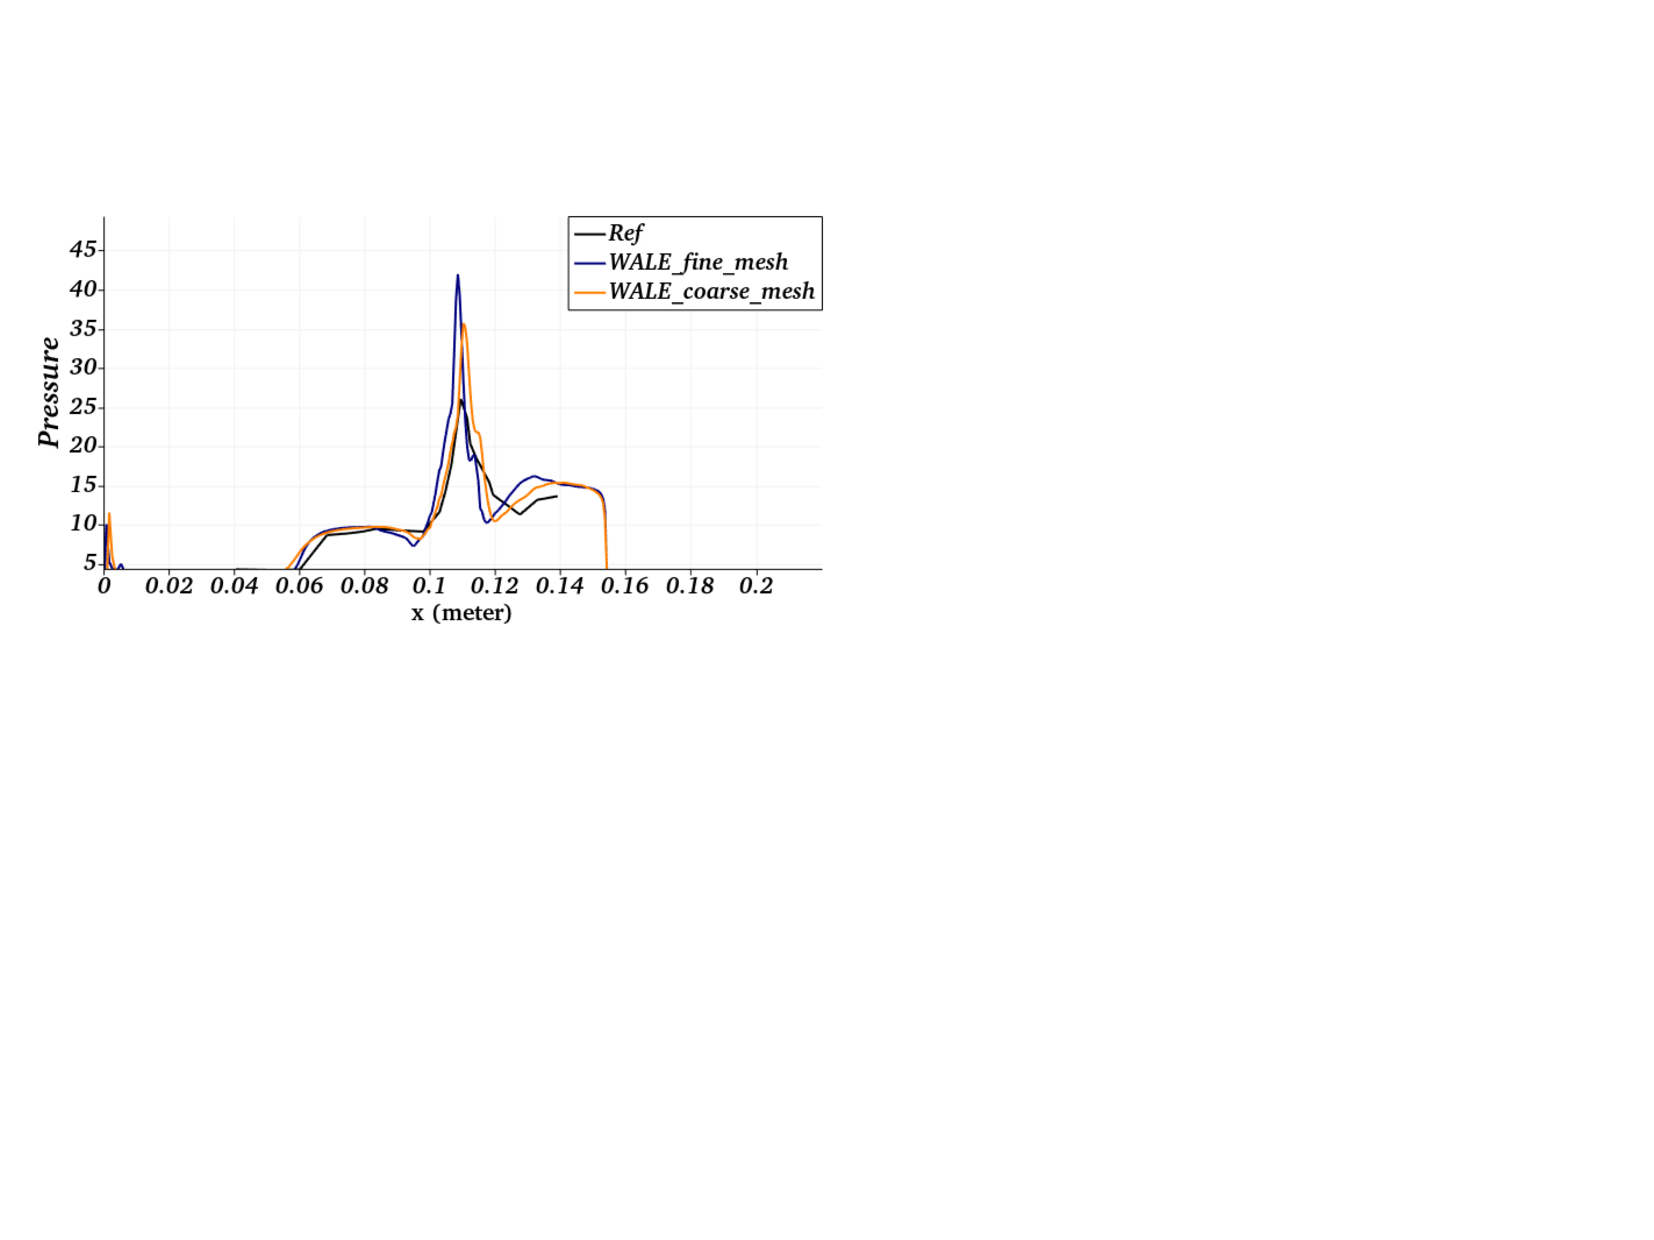
\includegraphics[width=0.47\linewidth]{chapter3_numerical_methods/pictures/double_cone_pressure.pdf} &
        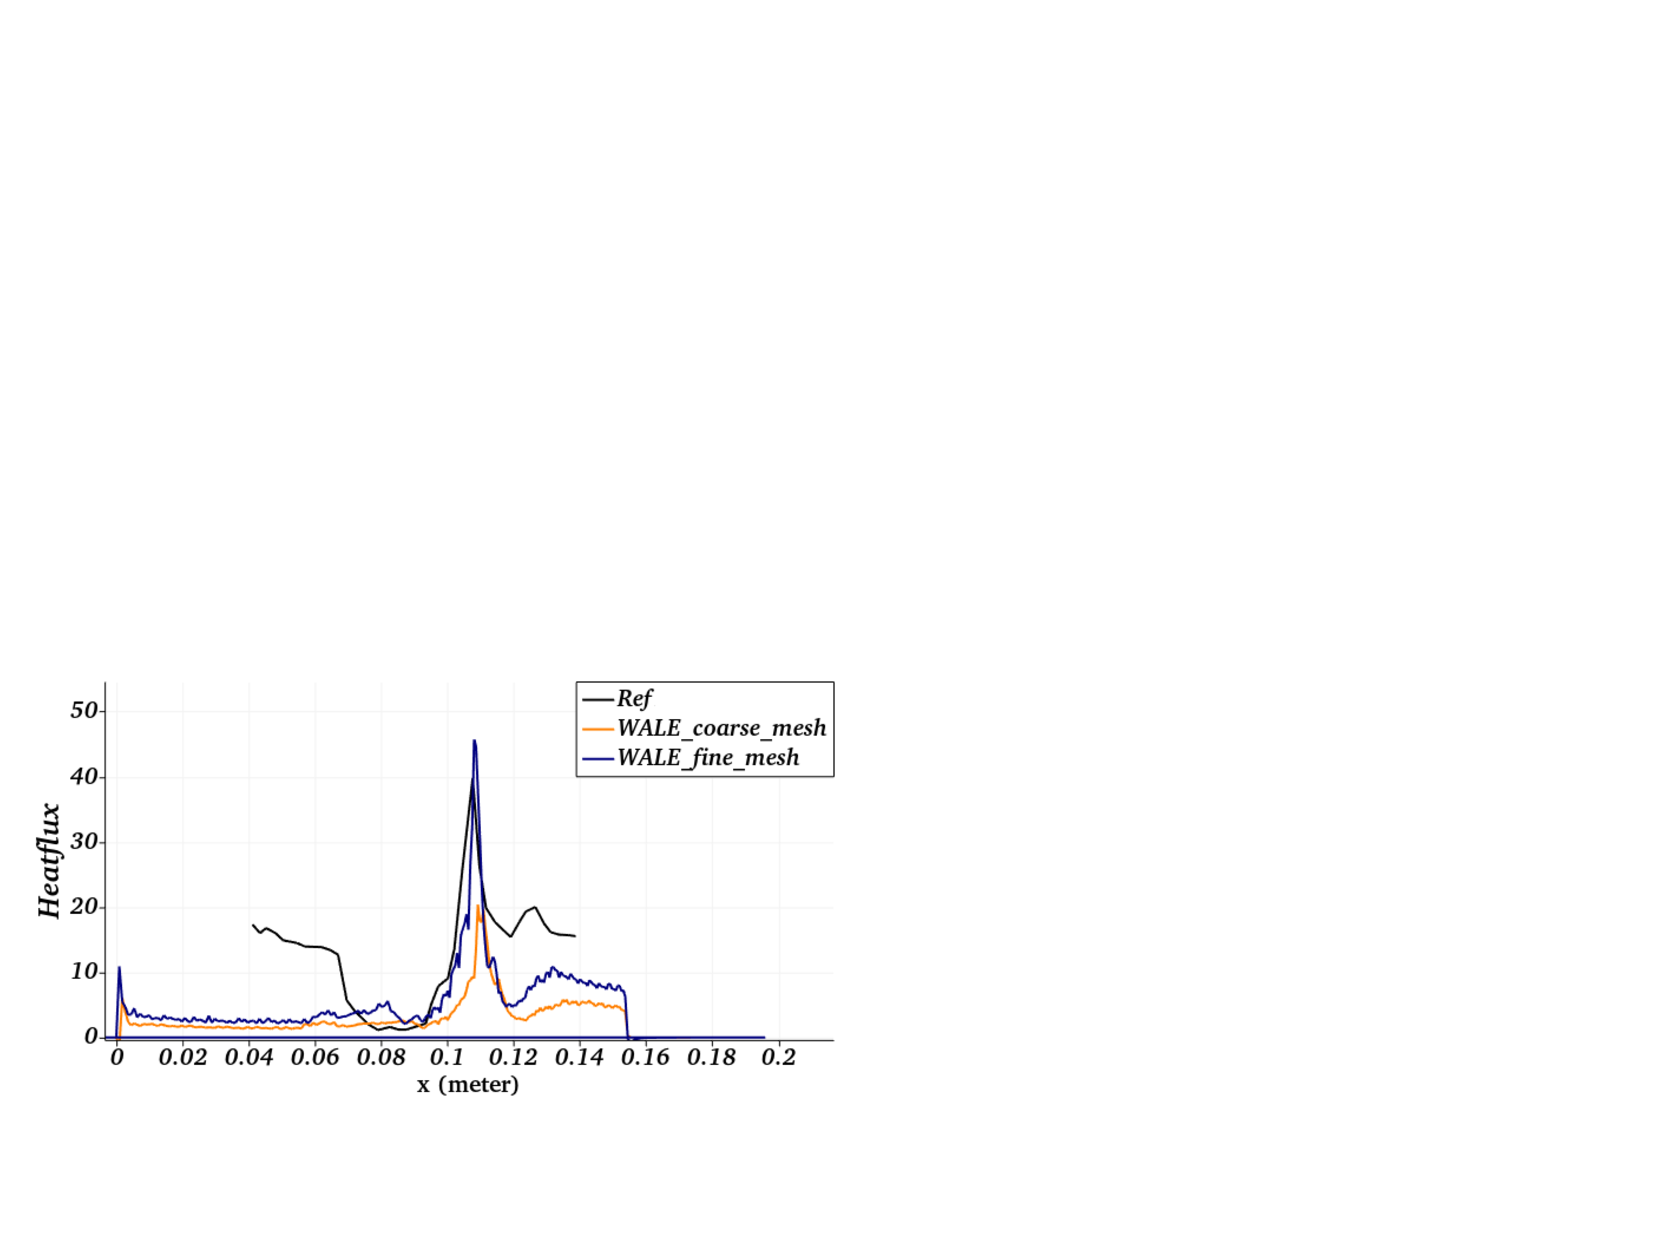
\includegraphics[width=0.47\linewidth]{chapter3_numerical_methods/pictures/double_cone_heat_flux.pdf} \\
        (a) & (b)
    \end{tabular}
    \caption{(a) Pressure coefficient and (b) heat flux obtained at the wall of the double cone.
    Comparison between the results obtained presently on the coarse and fine meshes (orange and blue line, respectively) and the reference solution from MacLean \emph{et al.} \cite{MacLean2014} (black line).}
    \label{fig:double_cone_comp}
\end{figure}


\subsection{Flow study around a double ellipsoid configuration}\label{ssec:test_ellipsoid}

The second immersed boundary condition testcase is the fully three-dimensional flow around a double ellipsoid shape \cite{Aymer1991} described mathematically by the following equations (see figure~\ref{fig:ellipse_geom}):

\begin{equation}
    \left\lbrace
    \begin{aligned}
        &x \leq 0,            &&\left( \frac{x}{0.06} \right)^2 + \left(\frac{y}{0.025} \right)^2 + \left( \frac{z}{0.015} \right)^2 &&= 1 \\
        &x \leq 0,\; z\geq 0, &&\left( \frac{x}{0.035} \right)^2 + \left(\frac{y}{0.0175} \right)^2 + \left( \frac{z}{0.025} \right)^2 &&= 1 \\
        &0 \leq x \leq 0.016, &&\left( \frac{y}{0.025} \right)^2 + \left( \frac{z}{0.015} \right)^2 &&= 1 \\
        &z \geq 0,            &&\left(\frac{y}{0.0175} \right)^2 + \left( \frac{z}{0.025} \right)^2 &&= 1
    \end{aligned}
    \right.
    \label{eq:double_ellipsoid_eqns}
\end{equation}

\begin{figure}[ht!]
    \centering
    \begin{tabular}{cc}
        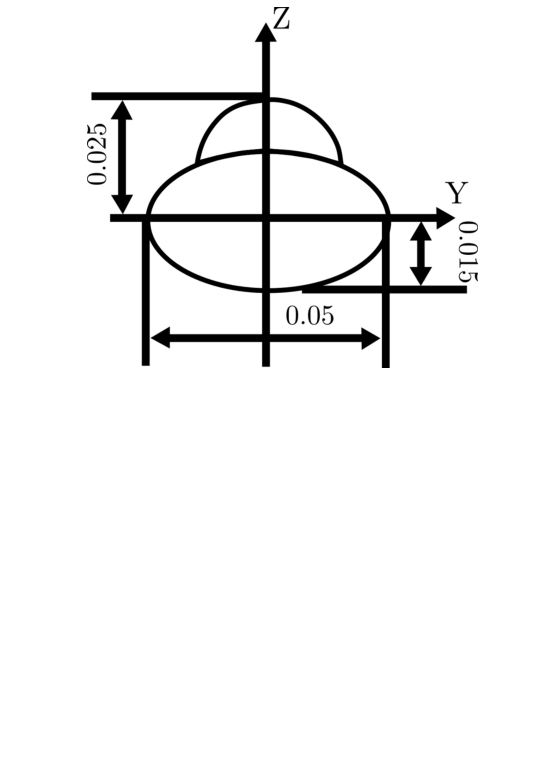
\includegraphics[width=0.35\linewidth]{chapter3_numerical_methods/pictures/ellipse_part1.pdf} &
        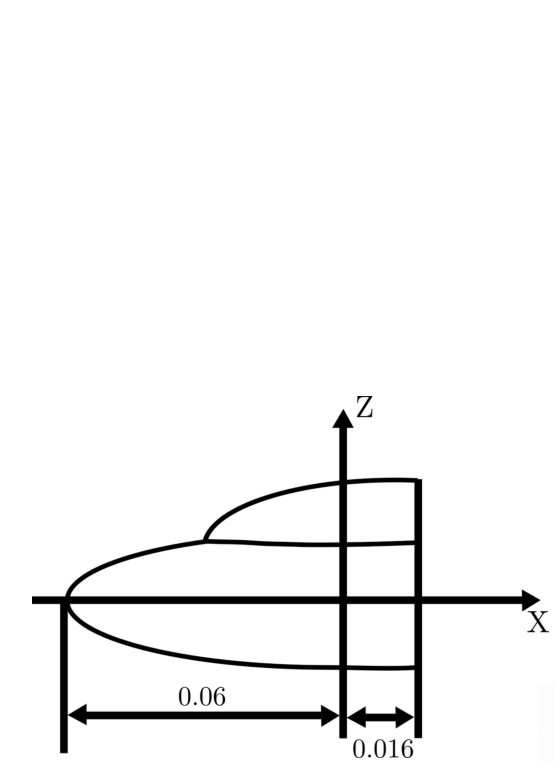
\includegraphics[width=0.45\linewidth]{chapter3_numerical_methods/pictures/ellipse_part2.pdf}
    \end{tabular}
    \caption{Geometrical details of the double ellipsoid configuration.}
    \label{fig:ellipse_geom}
\end{figure}

For that flow, the Mach number is set at $8.15$, the Reynolds number is set at $16.7\times 10^6$ and the freestream angle of attack is set at $30^{\circ}$.
The Cartesian mesh contains approximately $7\times 10^7$ cells, and the double ellipsoid object is tesselated using approximately $2\times 10^5$ triangles; the computation was conducted on $4096$ AMD Rome processors, using $2048$ MPI processes and $2$ OpenMP threads per process, and lasted approximately $48$ hours before the wall quantities could be said to be converged (see below).
Note that this computation, both in terms of manipulation of the immersed object and in terms of computational performance, is made possible only thanks to the two algorithms presented above in sections~\ref{sec:rasterization} and~\ref{sec:migratable_tasks} respectively - without massive parallelism, the time-to-results for this computation would have been unrealistic.

A first quantitative visualization of the flow is given in figure~\ref{fig:ellipse_3D}, where both numerical Schlieren imaging and three-dimensional isocontours of the Q-criterion are presented.
The strong shock waves can be clearly seen around the object whereas the wake seems characterized by multiple contact waves and large-scale turbulent structures that the LES simulation is able to capture, as expected.

\begin{figure}[ht!]
    \centering
    % \begin{tabular}{cc}
        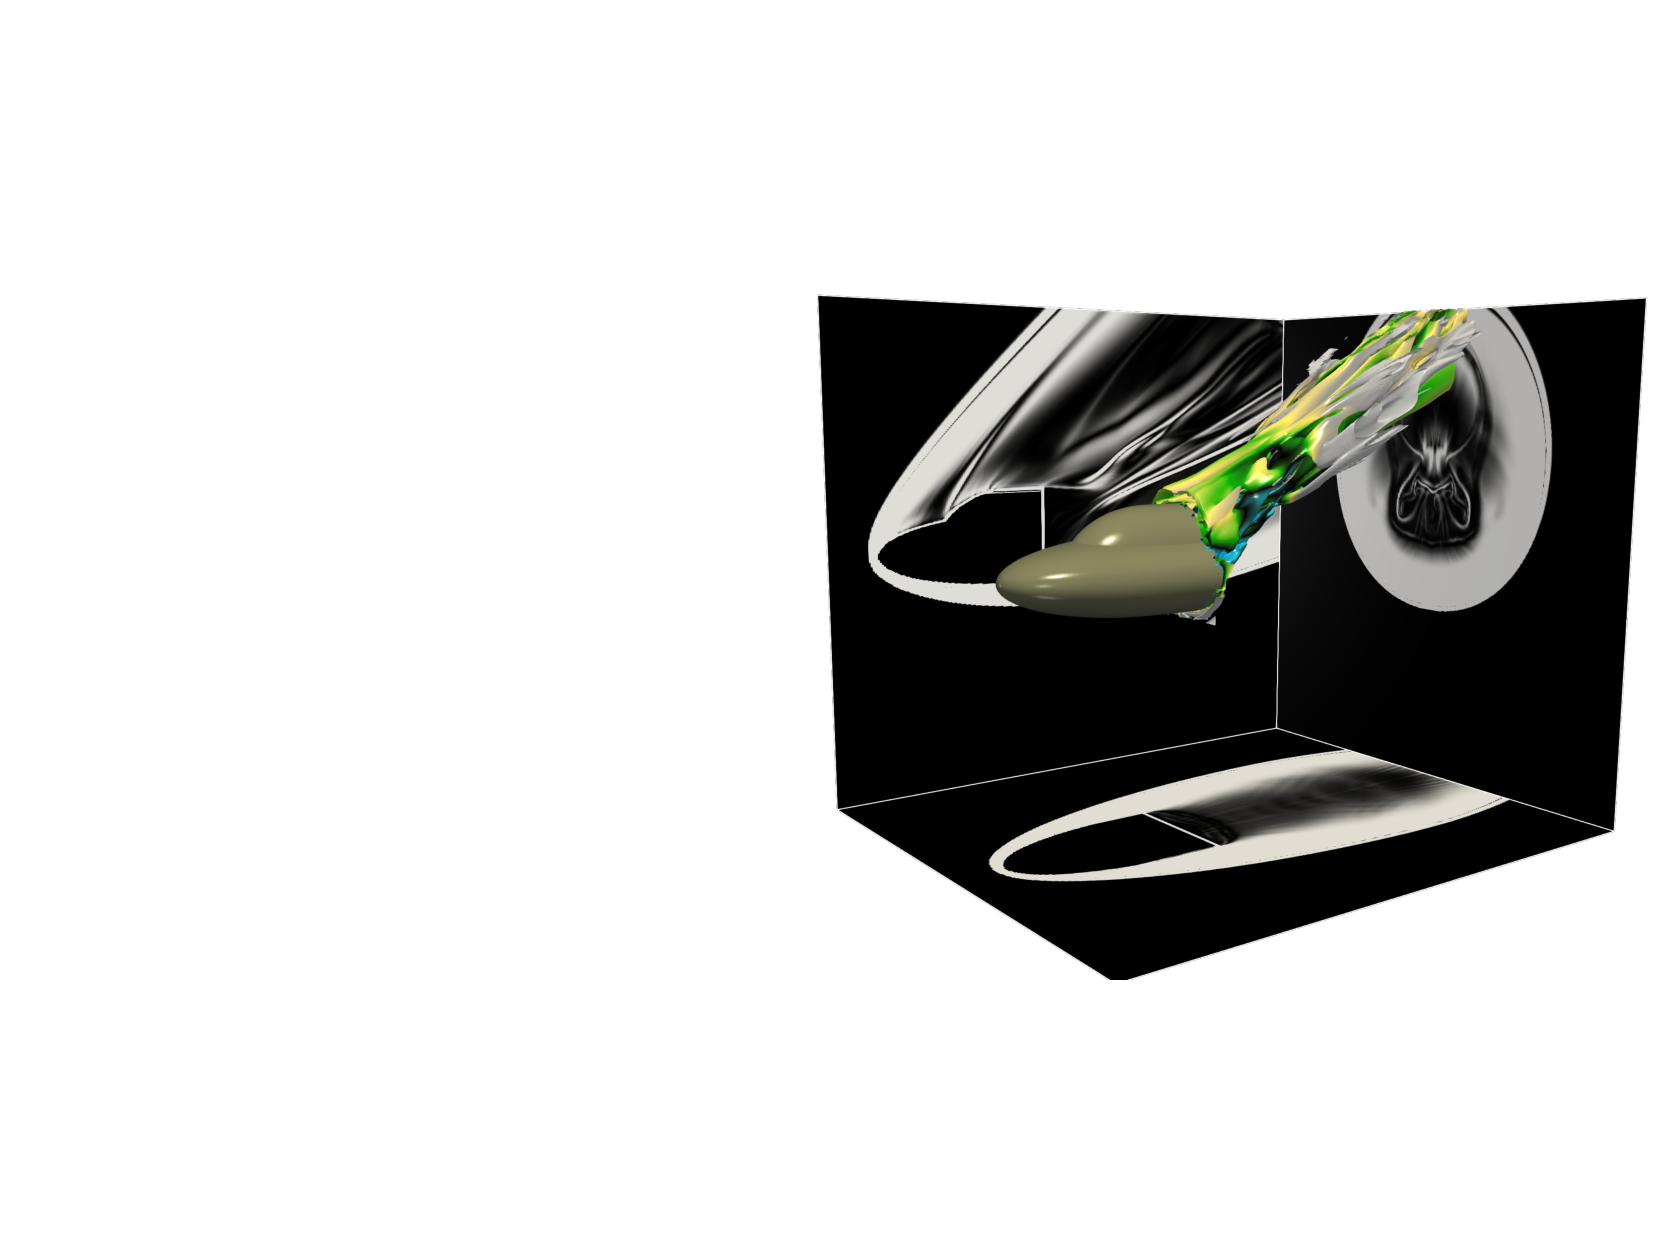
\includegraphics[width=0.65\linewidth]{chapter3_numerical_methods/pictures/ellipse_3Dview.pdf}% &
        % 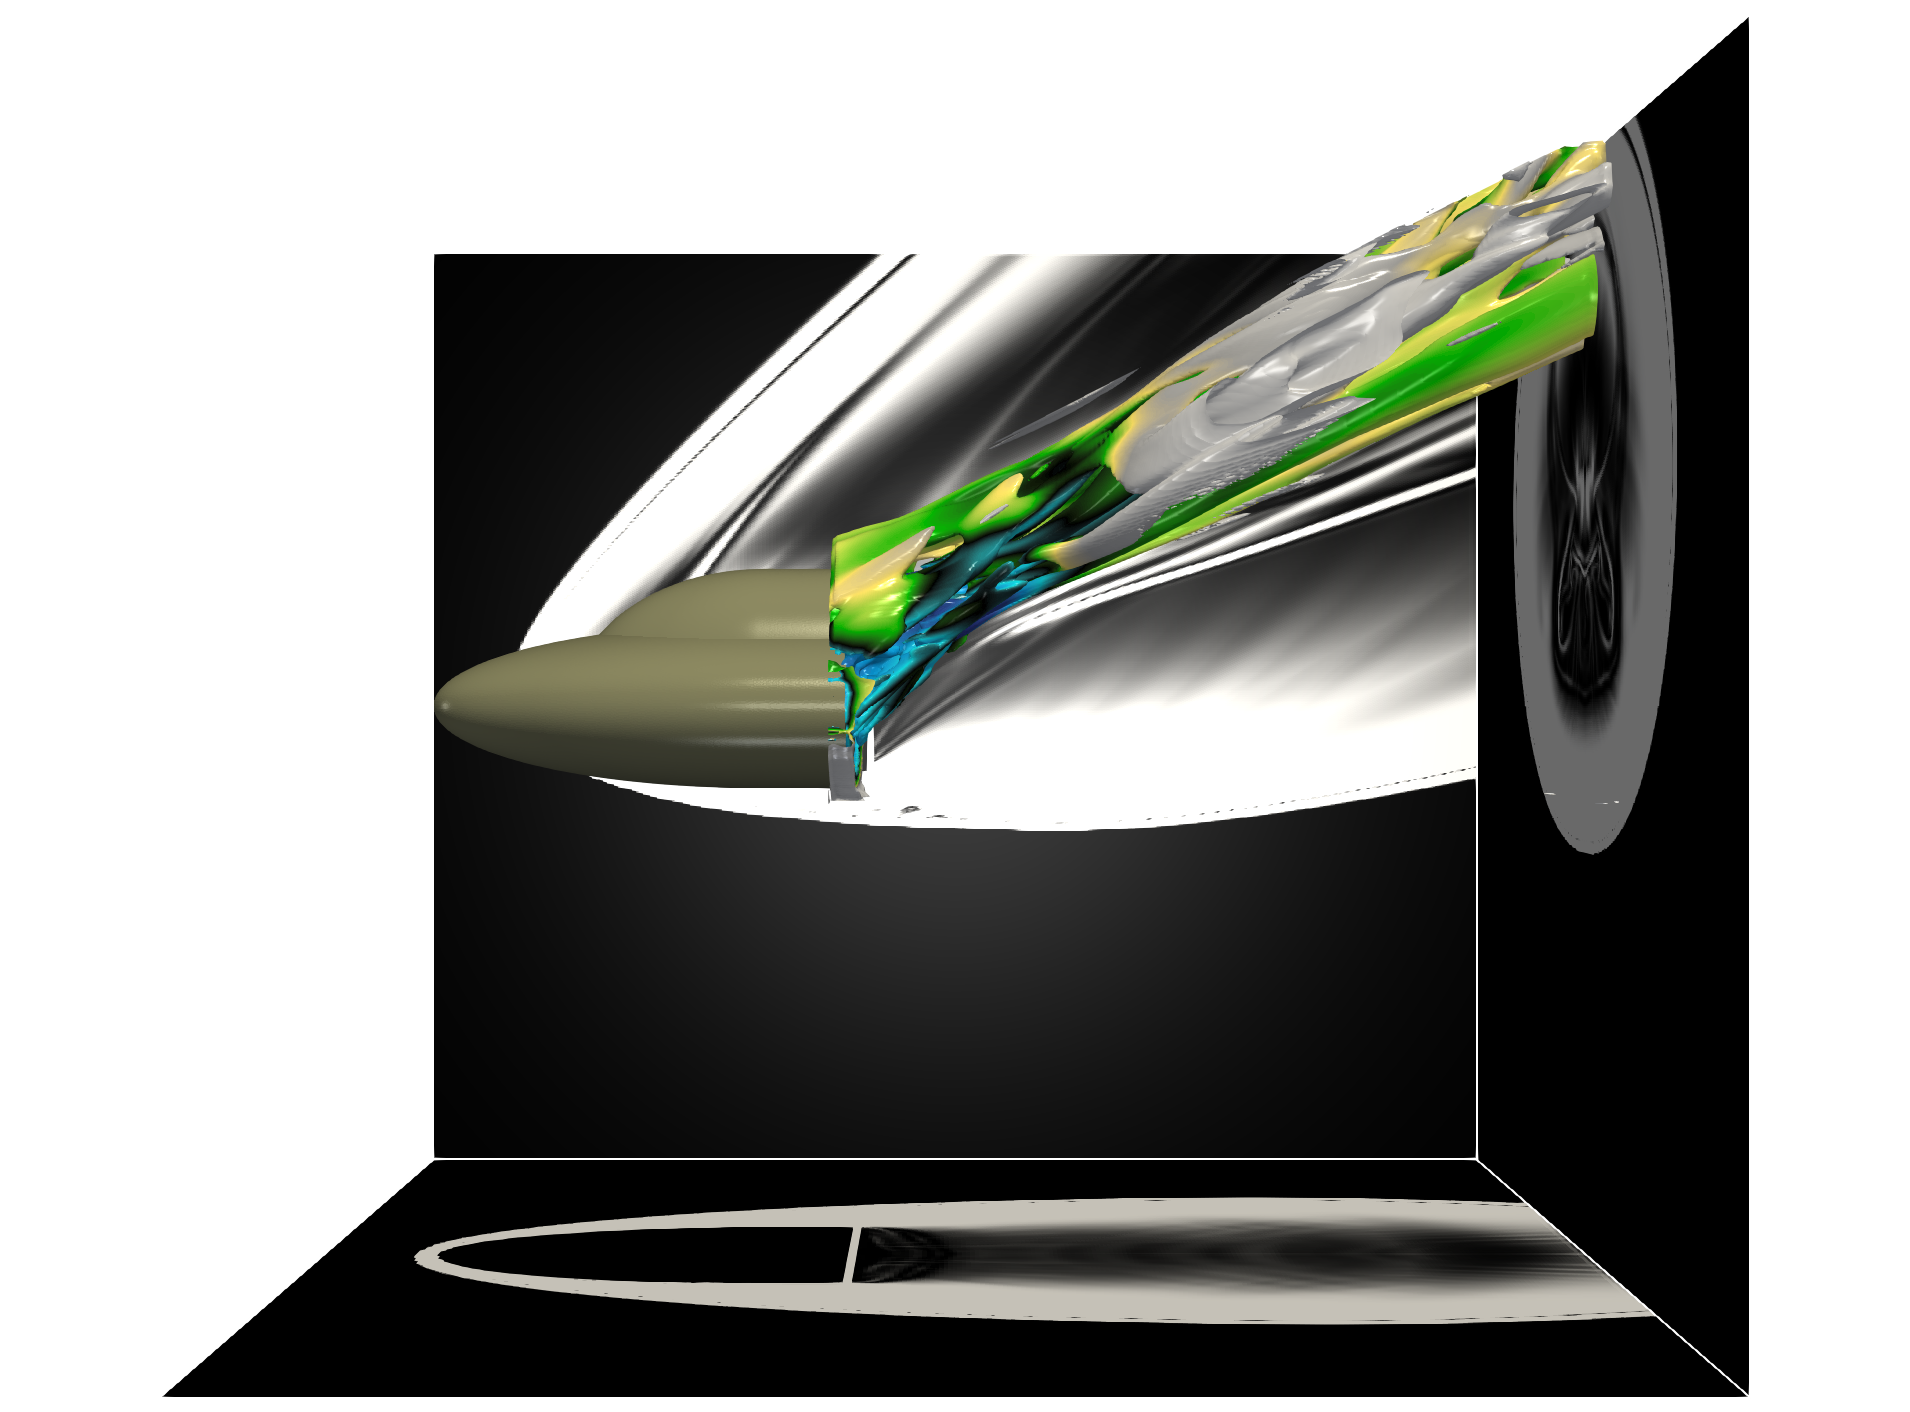
\includegraphics[width=0.45\linewidth]{ellipse_sideview.png}
    % \end{tabular}
    \caption{Illustration of the flow around the double ellipsoid immersed object with a $30^{\circ}$ angle of attack.
    The walls of the visualization domain are colored using the numerical Schlieren imaging technique, and the wake of the double ellipsoid is shown using isocontours of Q-criterion, colored by the magnitude of the vorticity.
    %Both a perspective (left) and a sideview (right) are displayed.
    }
    \label{fig:ellipse_3D}
\end{figure}

Similarly to the study conducted for the previous test case (see paragraph~\ref{ssec:test_double_cone}), figure~\ref{fig:ellipse_comp} presents the pressure coefficient and the Stanton number at the wall of the double ellipsoid.
The conclusions are similar to the ones for the double cone flow.
The pressure coefficient is satisfactorily predicted - the experimental data does not allow to conclude on the nature of the oscillations observed in the vicinity of the recirculation region (when the second ellipsoid starts, around $x \simeq 0.0$).
The heat flux accuracy is however fairly low again, mostly because of the lack of alignment between the Cartesian mesh and the object wall causing the boundary layers to be poorly described.
This phenomenon and possible fixes will be, as aforementioned, explored in a future study.

\begin{figure}[ht!]
    \centering
    \begin{tabular}{cc}
        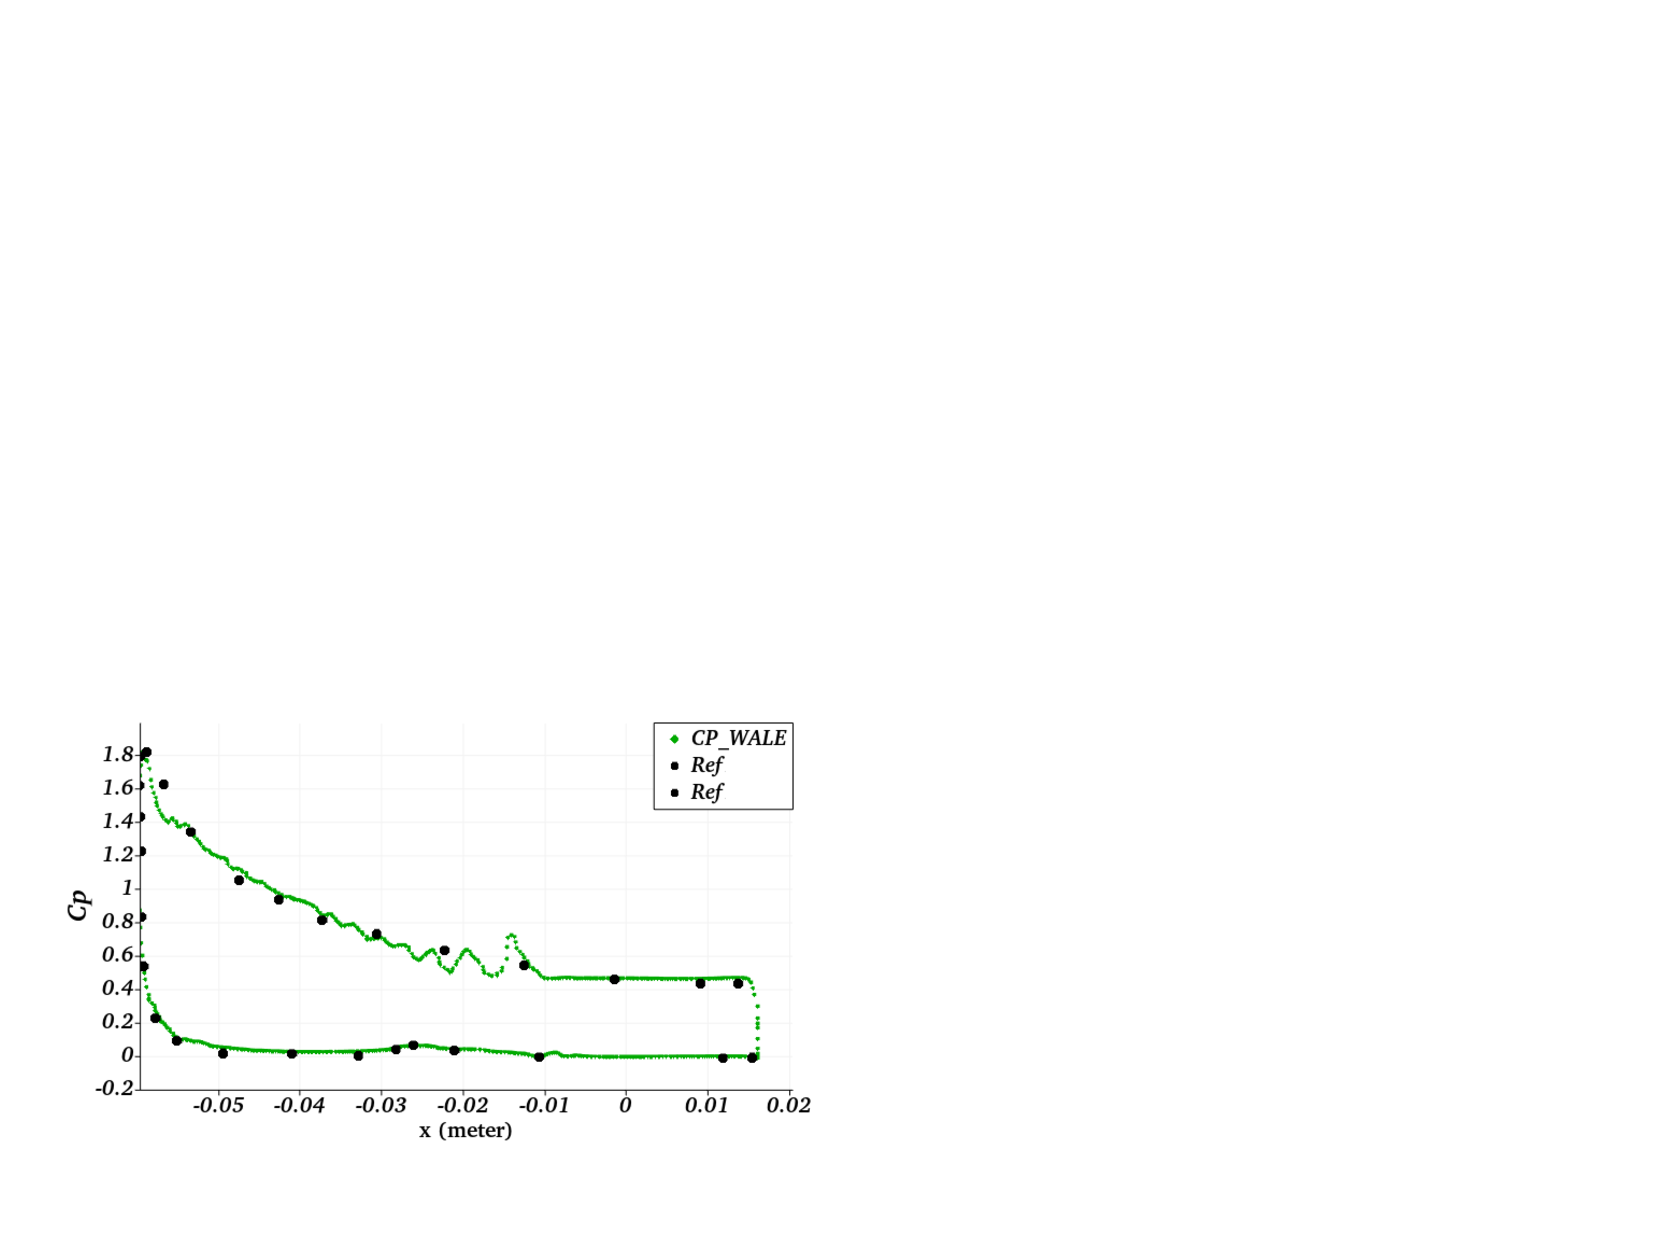
\includegraphics[width=0.45\linewidth]{chapter3_numerical_methods/pictures/ellipse_cp.pdf} &
        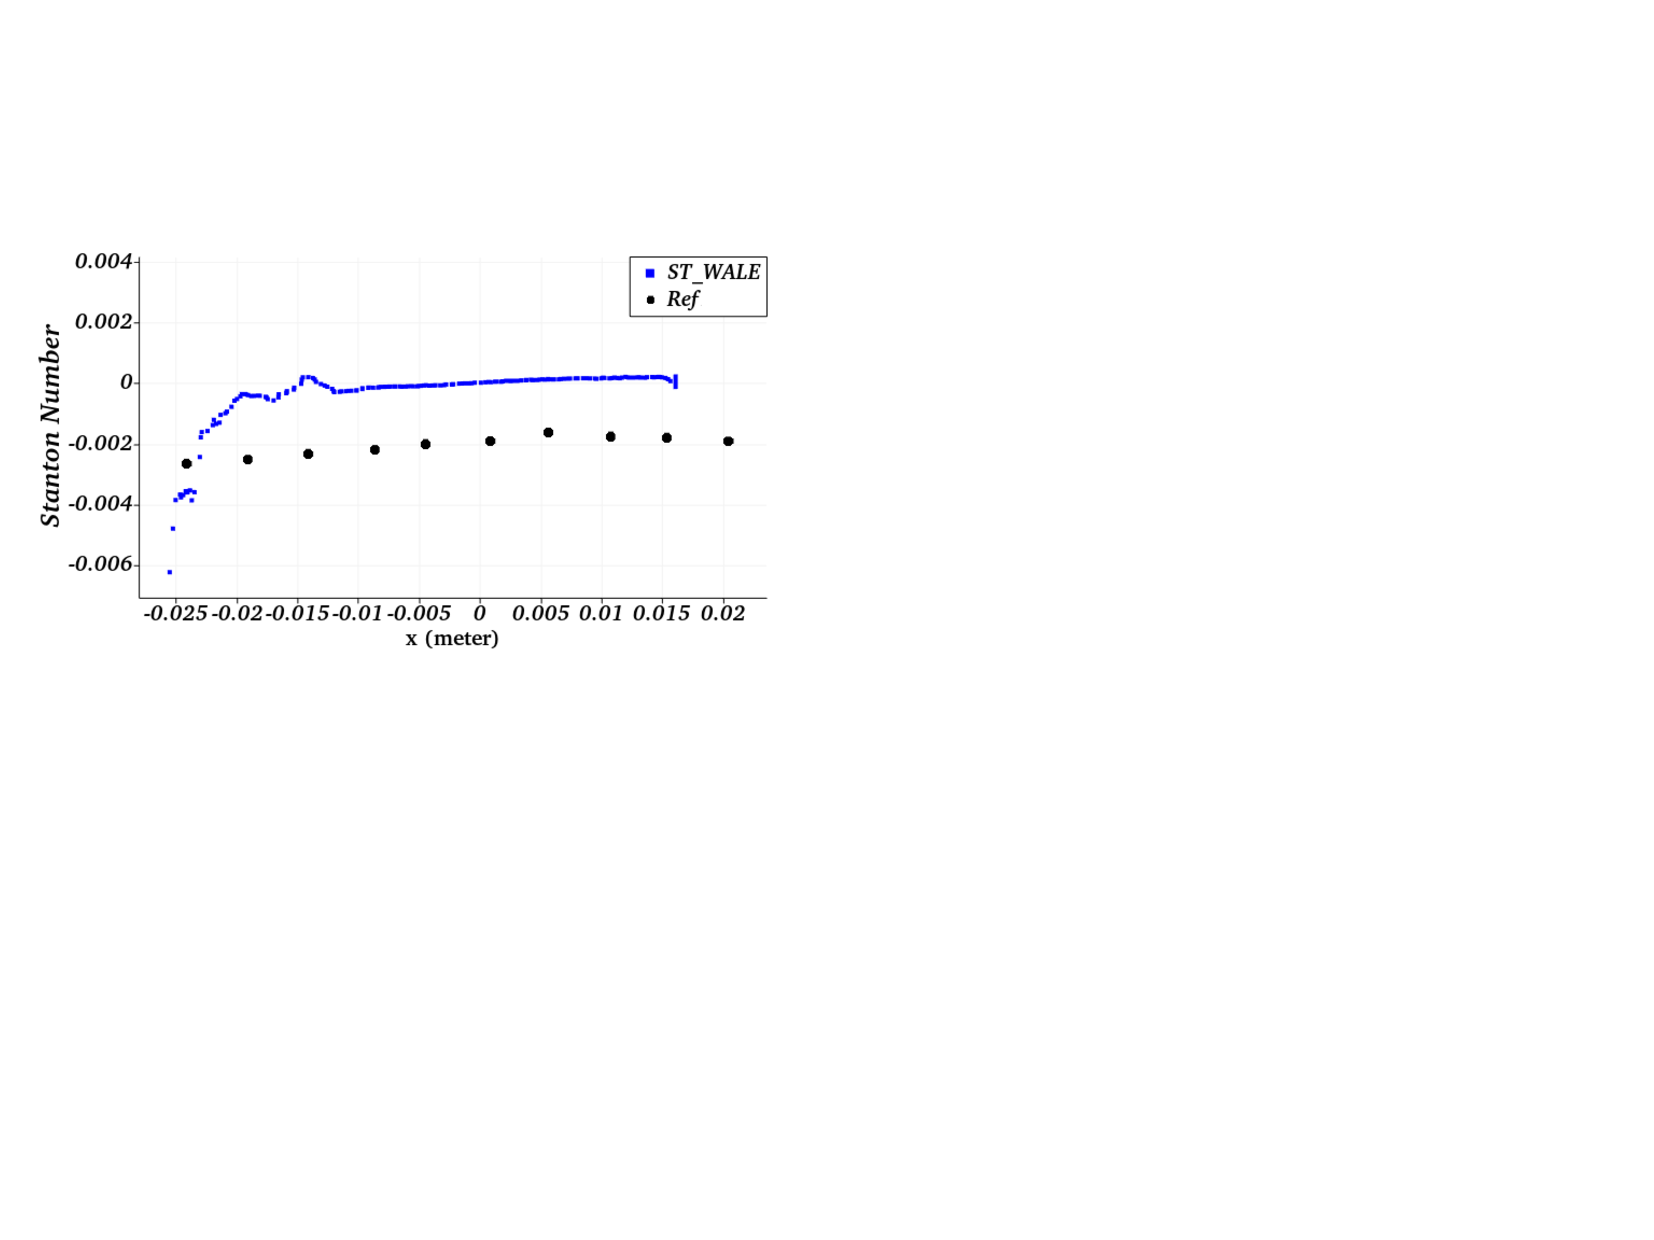
\includegraphics[width=0.45\linewidth]{chapter3_numerical_methods/pictures/ellipse_stanton.pdf} \\
        (a) & (b)
    \end{tabular}
    \caption{(a) Pressure coefficient on both the pressure and the suction sides and (b) Stanton number on the pressure side of the double ellipsoid.
    Comparison between the present computations (green and blue lines) and the experimental reference data (black dots) extracted from \cite{Aymer1991}.}
    \label{fig:ellipse_comp}
\end{figure}


\section{CONCLUSIONS}

In this paper, we present some work related to the immersed boundary method and in particular to the adaption of the method for massively parallel computations.
A novel algorithm based on the theory of computational geometry is introduced to drastically decrease the time necessary to identify a tesselated immersed body in a Cartesian box - from beyond $48$ hours to a few seconds.
The steps of this algorithm are detailed exhaustively and an example implementation of its non-trivial functions is provided.
Still in order to lift major limitations to conducting three-dimensional simulations involving immersed objects on massive clusters, a second algorithm is presented that make the interpolation step of the immersed boundary workflow possible for any number of MPI processes.
This algorithm represents the parallel extension of the works presented in \cite{BRIDELBERTOMEU2021} about an ENO-like least-square reconstruction mandatory to handle strong shocks in the vicinity of immersed bodies subject to hypersonic flows.

As those two new algorithms finally make massively parallel three-dimensional computations accessible with HYPERION, the improvement of the predictive capabilities of the code are then discussed.
Rather than conducting direct numerical simulations that stay, even today, unreachable because of their prohibitive computational cost at high Reynolds numbers, HYPERION is turned towards large eddy simulations (LES).
Preliminary axisymmetric and three-dimensional simulations conducted show that even if adequate subgrid-scale modeling allow for the prediction of large-scale turbulent structures on relatively coarse mesh, it is not enough to capture accurately the near-wall viscous phenomena.
The lack of alignment between the Cartesian grid (fluid grid) and the wall of the immersed body makes for poorly resolved boundary layers which, in turn, yield poor performance when it comes to predicting the viscous-driven wall quantities such as heat flux and shear stress.
A future study shall be dedicated to investigating these shortcomings and proposing solutions, perhaps axed towards the use of wall laws.
